%Dokumentklasse
\documentclass[a4paper,12pt,makeidx,twoside,openright,numbers=noenddot]{scrreprt}
\usepackage[left=3cm, right=2cm, bottom=2.5cm, top=3cm]{geometry}		% Formatierung der Seitenränder
%\usepackage[onehalfspacing]{setspace}							        % verwendet für größeren Zeilenabstand

% ============= Packages =============

% Dokumentinformationen


\usepackage[
	pdftitle={},
	pdfsubject={},
	pdfauthor={},
	pdfkeywords={},
	hidelinks
]{hyperref}



\usepackage[utf8]{inputenc}
\usepackage[ngerman]{babel}
\usepackage[T1]{fontenc}
\usepackage{units}
\usepackage{pdfpages}
\usepackage{listings}
\usepackage{svg}					% Zur Einbindung von scalable vector graphics
\usepackage{subcaption}				% Zum Einbinden von Untergrafiken
\usepackage[gen]{eurosym}			% Zur Verwendung des Eurozeichens
\usepackage{amssymb}
\usepackage{graphicx}
\graphicspath{{img/}}				
\usepackage{fancyhdr}				% Style Package für's Seitenlayout
\usepackage{color}					% anpassen von Farben
\usepackage{microtype} 				% schönerer Blocksatz!
\usepackage{calc}  					
\usepackage{enumitem}				% zb für align der description
\usepackage[font=small,labelfont=bf]{caption}
\usepackage[printonlyused]{acronym}	% für Abkürzungen
\usepackage{multicol}
\usepackage{booktabs}
\usepackage{textcomp}
\usepackage{listings}				% Einbindung von Code in LateX
\usepackage{setspace}
\usepackage{threeparttable} 		% für Fußnoten innerhalb einer Tabelle
\usepackage{tikz}
\usepackage{enumitem}
\usepackage{multirow}

% CODE PLUGIN!!
\usepackage{minted}

% verschiedene Schriftarten
%\usepackage{times} 				% times font
%\usepackage{palatino}			 	% Palatino font
\usepackage{lmodern}				% Lmodern sans und serif
%\usepackage{libertine}				% Linux Libertine und Biolinum

%\usepackage{fontspec}				% Nutzen in Kombination mit LuaLaTeX, um Systemschriften einzubinden
%\setmainfont{Georgia}				% beispielsweise Georgia, aber auch jede andere Schrift, die auf dem PC vorhanden ist


% zusätzliche Schriftzeichen der American Mathematical Society
\usepackage{amsfonts}
\usepackage{amsmath}

\usetikzlibrary{%
  arrows,%
  calc,
  shapes,
  arrows,
  shapes.misc,% wg. rounded rectangle
  shapes.arrows,%
  chains,%
  matrix,%
  positioning,% wg. " of "
  scopes,%
  decorations.pathmorphing,% /pgf/decoration/random steps | erste Graphik
  shadows%
}
\usepackage{amsmath}
\usepackage{relsize}

\usepackage[numbers, comma]{natbib}		% Einstellung des Zitierstils
%\bibliographystyle{myabbrvnat}			% Angepasster Stil für deutsche Sprache



\setcounter{secnumdepth}{3}				% Nummerierungsebene anpassen -> 3 = subsubsection werden nummeriert
\setcounter{tocdepth}{2}   				% gliederungsebenen im Inhaltsverzeichnis -> erstmal nur zur übersicht was nicht vergessen werden darf

\definecolor{deepblue}{rgb}{0,0,0.5}
\definecolor{deepred}{rgb}{0.6,0,0}
\definecolor{deepgreen}{rgb}{0,0.5,0}


% ============= Kopf- und Fußzeile =============
\pagestyle{fancy}

%% Formatierung der Kopf- und Fußzeile
\fancyhead{}
\fancyhead[RO,LE]{\thepage}
\fancyhead[RE]{\leftmark}
\fancyhead[LO]{\rightmark}
%%
\fancyfoot{}

\renewcommand{\headrulewidth}{0.4pt}		% Bei zweiseitigem Dokument ausschließlich Linie in Kopfzeile
\renewcommand{\chaptermark}[1]{\markboth{\thechapter\ #1}{}}
\renewcommand{\sectionmark}[1]{\markright{\thesection\ #1}}

% ============= Package Einstellungen & Sonstiges ============= 
% Besondere Trennungen
\hyphenation{Um-ge-bungs-tem-pe-ra-tur Um-ge-bungs-tem-pe-ra-tur-en Rauch-gas-tem-pe-ra-tur Aus-tritts-tem-pe-ra-tur}

% Einstellung wie Code innerhalb der Arbeit gesetzt werden soll:
\lstdefinestyle{Style}{
	columns=flexible,
	basicstyle=\ttfamily}
\lstset{ 
	backgroundcolor=\color{white},   % choose the background color; you must add \usepackage{color} or \usepackage{xcolor}; should come as last argument
	basicstyle=\footnotesize,        % the size of the fonts that are used for the code
	breakatwhitespace=false,         % sets if automatic breaks should only happen at whitespace
	breaklines=true,                 % sets automatic line breaking
	captionpos=none,                 % sets the caption-position to bottom
	commentstyle=\color{deepblue},   % comment style
	deletekeywords={...},            % if you want to delete keywords from the given language
	escapeinside={\%*}{*)},          % if you want to add LaTeX within your code
	extendedchars=true,              % lets you use non-ASCII characters; for 8-bits encodings only, does not work with UTF-8
	firstnumber=1,               	 % start line enumeration with line 1000
	frame=single,	                 % adds a frame around the code
	keepspaces=true,                 % keeps spaces in text, useful for keeping indentation of code (possibly needs columns=flexible)
	keywordstyle=\color{blue},       % keyword style
	language=Python,                 % the language of the code
	morekeywords={*,...},            % if you want to add more keywords to the set
	numbers=left,                    % where to put the line-numbers; possible values are (none, left, right)
	numbersep=5pt,                   % how far the line-numbers are from the code
	emphstyle=\color{deepred},
	%numberstyle=\tiny\color{mygray}, % the style that is used for the line-numbers
	rulecolor=\color{black},         % if not set, the frame-color may be changed on line-breaks within not-black text (e.g. comments (green here))
	showspaces=false,                % show spaces everywhere adding particular underscores; it overrides 'showstringspaces'
	showstringspaces=false,          % underline spaces within strings only
	showtabs=false,                  % show tabs within strings adding particular underscores
	stepnumber=2,                    % the step between two line-numbers. If it's 1, each line will be numbered
	stringstyle=\color{deepgreen},     % string literal style
	tabsize=2,	                   	 % sets default tabsize to 2 spaces
	title=\lstname                   % show the filename of files included with \lstinputlisting; also try caption instead of title
}
% nicht einrücken nach Absatz
\setlength{\parindent}{0pt}
\usepackage{parskip}		 			% verhindert einrücken und setzt einen kleinen Absatz

\renewcommand{\arraystretch}{1.2}		% Abstand innerhalb der Tabellen einstellen

\usepackage{natbib}

\newcommand*{\mytitle}{Analysing the Characteristics of Neural Networks for the Recognition of Sugar Beets} % Titel
\newcommand*{\myinstitute}{Applied University of Hamm-Lippstadt} % Institut


\newcommand*{\myauthor}{Luca Brodo} % Autoren
\newcommand*{\myreporttype}{Bachelor thesis} % Bericht-Typ
\newcommand*{\mygraduation}{Bachelor of Engineering} % Vollständige Anschrift



\newcommand*{\firstexaminer}{Prof. Dr. Stefan Henkler} % Ort
\newcommand*{\secondexaminer}{Prof. Dr. Achim Rettberg} % Ort
\newcommand*{\thirdexaminer}{Dipl.-Wirt.-Inf. Kristian Rother} % Ort
\newcommand*{\mydate}{\today} % Datum


% ============= Dokumentbeginn =============

\begin{document}

% Seiten ohne Kopf- und Fußzeile sowie Seitenzahl
\pagestyle{empty}

\begin{center}
\begin{tabular}{p{\textwidth}}

\begin{center}
	
\includegraphics[scale=0.12]{img/HSHL_Logo_horizontal_RGB_lightgreen_darkblue_mit-Schutzraum_ENG.jpg}
\end{center}


\\

\begin{center}
\LARGE{\textbf{
\mytitle\\[1cm]
}}
\end{center}

\\


\begin{center}
\large{\myinstitute\\}

\end{center}

\\\\

\begin{center}
\textbf{\Large{\myreporttype}}
\end{center}


\begin{center}
for the attainment of the academic degree\\
\mygraduation
\end{center}

\\\\

\begin{center}
submitted by
\end{center}

\begin{center}
\large{\textbf{\myauthor}} \\
% \small{geboren am 01.01.0001 in Entenhausen}
\end{center}

\\\\
\begin{center}


Electronic Engineering\\
Mat.Nr.: 2180015\\
luca.brodo@stud.hshl.de\\
\vspace{0.5cm}
\large{\mydate}


\end{center}

\\
\\
\\

\begin{center}
\begin{tabular}{lll}
\textbf{First supervisor:} & & \firstexaminer\\
\textbf{Second supervisor:} & & \secondexaminer\\
\end{tabular}
\end{center}

\end{tabular}
\end{center}	% Einbinden der Titelseite
\newpage 					% Um Seite nach der Titelseite einzubinden -> bei eigener Titelseite und nicht der Latex-Version erforderlich
\thispagestyle{empty}
\quad 
\vfil
\hfil \textit{} \hfil
\vfil 
%\pagenumbering{arabic}
 

\cleardoubleoddpage



\chapter*{Affidavit}
I, \myauthor, herewith declare that I have composed the present paper and work by myself and without use of any other than the cited sources and aids. Sentences or parts of sentences quoted literally are marked as such; other references with regard to the statement and scope are indicated by full details of the publications concerned. The paper and work in the same or similar form has not been submitted to any examination body and has not been published. \\
Lippstadt, \today\\[.6cm]
\myauthor\\
\hfil
\rule[0.5em]{20em}{0.5pt}


\begin{abstract}
Sugar beets plantations are perfect candidates for the application of smart farming methodologies. While bringing innumerable benefits, most of the proposed solutions are based on the recognition of the plants to increase yield and increase sustainability of the plantation. As the recognition task is usually tackled using Convolutional Neural Networks (CNNs), the unpredictability of them imposes great challenges to engineers. In this paper, we focus on the analysis of the networks to find correlations between their characteristics to be reliable and predictable in time, with the aim of making sugar beet recognition more transparent. We will start our investigation from defining and analysing the characteristics we are interested in. This step allows us to find appropriate techniques to create a benchmark tool for the analysis neural networks. We will use this tool and the characteristics we define to investigate the training and inference process of eight models using two different dataset.\\
Although these two use cases show promising results, as we are only going to focus on analysing models and finding correlations between some of their characteristics, this paper is only the first milestone towards using this correlation to optimize smart farming applications to improve the production and sustainability of the plantations around the world. 
\end{abstract}
\renewcommand*\listfigurename{List of Figures}
\renewcommand*\contentsname{Table of Content}
\renewcommand*\listtablename{List of Tables}

\newcommand\gw{8}
\newcommand\gws{8}
%\setcounter{tocdepth}{3}
%\setcounter{secnumdepth}{3}


\tableofcontents			%Inhaltsverzeichnis
\listoffigures		%Verzeichnis aller Bilder
\listoftables				%Verzeichnis aller Tabellen




%\chapter*{Abkürzungsverzeichnis}
%	\begin{acronym}[4GDH]	% Zur Formatierung hier die längste Abkürzung des Verzeichnisses eintragen
%		\acro{4GDH}{4th Generation District Heating} 	
%	\end{acronym}
\renewcommand{\figurename}{Fig.}
\renewcommand{\tablename}{Table}
\pagestyle{fancy}
\chapter{Motivation}
The seemingly unstoppable growth of global population compounded by climate change is putting an enormous pressure on the agricultural sector. As estimated by the World Resources Institutes (WRI), the number of people on our planet will reach an astounding 10 billion by 2050  \cite{ayaz_internet--things_2019} and, as a result, the agricultural production must double to keep up with the demand \cite{singh_machine_2016}. However, the agricultural sector is facing immense challenges due to plant diseases, pests and weed infestation and in these times, like never before, the switch to a more sustainable model seems inevitable. The main target of sustainable farming is to increase yield while reducing reliance on herbicides and pesticides; therefore trying to target treatments only to plants that specifically require it by monitoring key indicators of each individual crop, a technique usually referred to as precision farming. This technique is notoriously time and energy consuming if done manually and therefore usually discarded in favor of more traditional methodologies. \cite{lottes_effective_2016}\\
In the last years there has been, however, an increased focus on integrating cutting-edge technology with precision farming precision farming to improve quality and quantity of agricultural production, while at the same time lowering the inputs significantly \cite{islam_review_2021}.  This system is also known as ''smart farming''.  This system is based on the adoption of autonomous robots, which could be both wheeled robots and Unmanned Aerial Vehicles (UAVs), and it has been enabled by the astonishing advancements in the field of the Internet of Things (IoT). \\
IoT is the key technology behind smart farming and allows to add value to the data collected by automated processes by ensuring data flow between different devices  \cite{islam_review_2021}.  More importantly, IoT allows more cost-efficient and timely production and management practices, as showed by  Glaroudis et al. in\cite{glaroudis_survey_2020}, and at the same time the reduction of the inherent climate impact by enabling real-time reactions to infestations,  such as weed, pest or diseases, and by enabling a more adequate use of resources such as water, pesticides or agro-chemicals.\cite{islam_review_2021}
In other words, IoT makes precision farming not only more efficient in terms of both money and resources, but even more sustainable than other traditional farming methods. \\
One of cultivations which will benefit immensely by the adoption of smart farming is the sugar beet. The \textit{Beta vulgaris L},depicted in Fig. \ref{fig:sugar_beet}, commonly referred as sugar beet, is ranked as the second most cultivated  sugar crop all over the world next to sugarcane\cite{bhadra_weed_2020}. As showed by May in \cite{may_economic_2003}, being a slow-growing crop early in the season \cite{bhadra_weed_2020}, this plant seems to be a very poor competitor against weed, backed up also by Schweizer's researches, which reports that sugar beet root yields can be reduced by 26–100\% by uncontrolled weed growth.  \cite{schweizer_weed_1989}\\
\begin{figure}[ht]
	\centering
	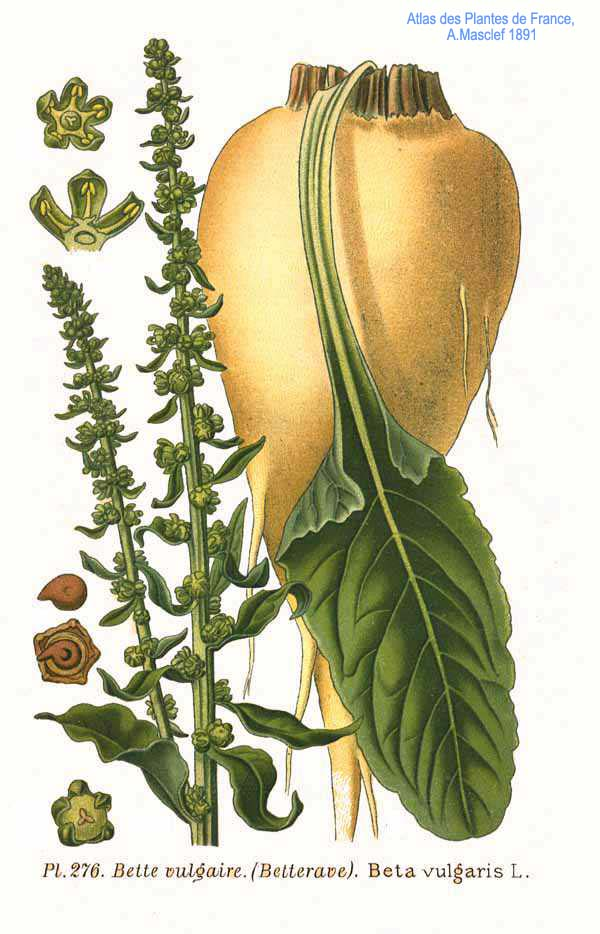
\includegraphics[width = 5cm]{img/276_Beta_vulgaris_L.jpg}
	\caption[Representation of a sugar beet plant]{Representation of a sugar beet plant \cite{masclef_sugar_1891} }{\centering}
	\label{fig:sugar_beet}
\end{figure}
\section{Smart Farming in Sugar Beet Plantations}
An approach based on smart farming could reduce the effect of weeds infestations on sugar beet plantations and  increment the yield and the sustainability of said plantation.\\
As a matter of fact, even though tractors and hand labour are still vastly used for weed management, since the 50s, herbicides have been the most used method of weed management in sugar beets farms (\cite{cioni_weed_2010}) and, apart from the well known environmental damage, which the use herbicides leads to, another implication is the effect that they have on the sugar beet crops. Most of the selective herbicides have influence on sugar beet growth, with early symptoms showing on the leaves, and this can reduce the yield. \cite{petersen_review_2004}\\
To optimize and remove the effects of pesticides, the new frontier for weed management is to automatize the more traditional mechanical techniques (\cite{raja_real-time_2020}, \cite{frasconi_design_2014},\cite{machleb_sensor-based_2021}).\\
Mechanical techniques and even techniques which use selective spraying of herbicides, however, require that the sugar beet is localized before they can be applied to avoid ruining the plantation. In the research field,a lot of proposed solutions employ Convolutional Neural Networks (CNNs) in the recognition task (\cite{gao_deep_2020},\cite{suh_transfer_2018},\cite{ramirez_deep_2020}, \cite{milioto2017real},\cite{agriculture11111111}).\\
Neural Networks,however, impose great challenges to the developers. For example, in real time applications, classification time is of the highest importance since it effects the ability to respect deadlines. Furthermore, the performances of CNNs is influenced by many factors, like for i.g. training time or the data-set used for training.\\ %Table \ref{tab:models_ex_comp} shows an example of different architectures trained to recognize weed in a sugar beet plantations and how their performances can vary. \\ 
Being able to predict the performances of NNs before their deployment will allow engineers to precisely model the application to tailor them for the NN of their chose. \\
In this paper, we are going to investigate whether it is possible to make those predictions by empirically studying some of the metrics which can influence NNs' performances and find correlations amongst them in order to be able to be precise, scalable and predictable in time. An the result of our investigation, we aim to develop a toolbox for the employment of NNs in sugar beet recognition.

\section{Organization of the Paper}
In order to achieve the aforementioned goal, we will first analyse the main characteristics of Neural Networks in chapter number \ref{char_nn}. This will allow us to pose the foundations for our further studies, since it is essential to have a proper knowledge of what can influence the recognition of sugar beets .\\
Subsequently, in chapter number \ref{ana_models}, we will study how we can benchmark neural networks to obtain the measurements we need to find the correlations. Benchmarking is a notoriously insidious task, however at the end of our study, we will be able to create a tool to measure performances and analyse Neural Networks in a precise and reproducible way.\\
Finally, with the help of our tool, in chapter \ref{ana_char} we will profile Neural Networks with fairly different architectures to identify correlations between their metrics so that we will be able to optimize the recognition of sugar beets. 

\chapter{Related Work}
Multiple proposed solutions in the academia for sugar beet recognition use Convolutional Neural Networks to recognize both weed and sugar beets in a plantation. The solutions we are going to consider have been studied more thoroughly in \cite{project_work}. \\
\textit{Gao et al. } in \cite{gao_deep_2020} developed a CNN based on the popular tiny YOLOv3 framework (\cite{9074315}), but with modifications for increased performances. They added two more layers for better feature fusion and reduced the number of detection to two, rather than the standard 3 for YOLO, since the images of sugar beets they collected were generally similar in size.\\
Instead of using only images collected from the field, the authors developed a tool to synthetically generate over 2000 images of sugar beets, which, according to them, allowed to save time and resources. The model they developed has an accuracy of \textasciitilde83\% with an average inference time of 6.48ms.\\
\textit{Suh et al.} in \cite{suh_transfer_2018} focused their study on the Alexnet architecture (section \ref{sec:Alexnet}) considering three approaches: AlexNet as a fixed feature extractor, modified and fine-tuned AlexNet as a binary classifier, modified and fine-tuned AlexNet as a fixed feature extractor. An overview of the three approaches can be seen in table \ref{tab:alexnet_comparison}. 
\begin{table}[h]
\begin{tabular}[h]{ c c  c c c}
\hline
Approach & Highest accuracy & Training time (s) & Classification time (s) &\# of Images\\
\hline
  1	&	97\%		& 	13.3		&	0.016	&	1100 \\
  2 	& 	98.0\% 	& 	656.4	&	0.012	&	900 \\
  3 	& 	96.7\% 	& 	195.8 	&	0.0130s 	& 	300\\
  3 	& 	97.3\% 	& 	581.4 	&	0.0130s 	& 	800\\

\end{tabular}

\caption[Comparison between the three different approaches using AlexNet]{Comparison between the three different approaches using AlexNet \cite{suh_transfer_2018}}
 \label{tab:alexnet_comparison}
\end{table}

Authors of \cite{suh_transfer_2018} also provide a comparison between six fine-tuned deep networks, namely AlexNet, VGG-19, GoogLeNet, ResNet-50, ResNet-101 and Inception-v3, summarized in table \ref{tab:models_ex_comp}.\\
Both table \ref{tab:alexnet_comparison} and \ref{tab:models_ex_comp} show how differently NNs perform in similar settings when some metrics are changed. For example, in table \ref{tab:models_ex_comp}, we can see that both Resnet50 and Resnet101 achieve different inference time when trained for different numbers of epochs, i.e. with different training time.\\
\begin{table}[h]
\centering
\begin{tabular}{|c| ccc|}
  \hline
 Network &Accuracy& Training time   &Classification time   \\
 \hline
 &\multicolumn{3}{c|}{20 Epoch}\\
 \hline
AlexNet &97.9\%& 9.0min   &0.0038s    \\
VGG-19 &98.4\%& 37.4min   &0.0130s  \\
GoogLeNet &97.0\%& 23.8min  &0.0033s \\
ResNet-50 &96.2\%& 40.3min  &0.0072s\\
ResNet-101 &97.5\%& 106.6min   &0.0118s \\
Inception-v3 &90.8\%& 88.7min &0.0088s \\
\hline
&\multicolumn{3}{c|}{30 Epoch}\\
\hline
AlexNet & 97.7\% &15.6min &0.0040s     \\
VGG-19 &98.7\% &71.4min&0.0124s  \\
GoogLeNet  &97.3\% &36.9min& 0.0035s     \\
ResNet-50 & 97.2\% &69.8min&0.0075s      \\
ResNet-101 & 98.5\% &162.0min&   0.0111s   \\
Inception-v3 & 94.8\% &133.0min   & 0.0086s  \\
\hline
\end{tabular}
\caption[Comparison between the classification performance of different Neural Networks]{Comparison between the classification performance of different Neural Networks \cite{suh_transfer_2018}}
 \label{tab:models_ex_comp}
\end{table}
Regarding the study of Neural Network performances, both academic and industrial organizations have already developed numerous benchmark solutions to evaluate the behaviour of NNs under different workloads and on different devices. For example, authors of \cite{luo2020comparison} and \cite{ignatov2019ai} have proposed benchmarks of NNs specifically for mobile devices. \textit{Hendrycks et al.} in  \cite{hendrycks2019benchmarking} developed a benchmark to assess the robustness of image classifiers under condition of perturbations. \\
\textit{Reddi et al.} in  \cite{reddi2020mlperf} propose a benchmark, namely MLPerf, to evaluate inference of Machine Learning system under various workloads. They divided workloads under high level tasks, such as image classification, and they provide a reference model for it. \\
\textit{Zou et al. } in \cite{8573476}, among other contributions, proposed a benchmark suite to analyse NNs' training time of eight different state-of-the-art models under six different application domains. The metrics they collect during profiling are:
\begin{description}
  \item[\textbf{Throughput}] \hfill\\ Throughput is defined as the amount of input samples processed by the networks. This metric is relevant because, contrary to inference, it is not latency sensitive.   
  \item[\textbf{GPU utilization}] \hfill \\ They define the GPU utilization as the fraction of time in which the GPU is busy, it is calculated as follows:
  \begin{equation}
      GPU\;Utilization = \dfrac{GPU\;Active\;Time\times100}{total\;elapsed\;time}%
  \end{equation}
  
  \item[\textbf{FP32 utilization}] \hfill \\ This metric refers to the percentage of floating operations done during training, since typically training DNNs is performed using single precision floating point operations (FP32). This metric measures how effectively the GPU resources are used. It is calculated as:
  \begin{equation}
      FP32\;Utilization = \dfrac{actual\;flop\;counting\;during\;T\times100}{FLOPS_{peak} \times T}%
  \end{equation}
  Where:
  \begin{itemize}
  \item $FLOPS_{peak}$ is the GPU theoretical peak analysis
  \item $T$ is the period of time in seconds that the GPU is active
  \end{itemize}
  \item[\textbf{CPU utilization }] \hfill\\ This is calculated as the average utilization of each CPU core:
  \begin{equation}
      \dfrac{\sum_{c} total\;time\;of\;active\;core\;c \times 100}{CPU\;core\;count \times total\;elapsed\;time}%
    \end{equation}   
    \item[\textbf{Memory consumption }] \hfill\\ The memory consumed by the NNs during training
\end{description}
Although the aforementioned benchmarks have brought many advancements on the field, they are not meant to be used to study the characteristics of the NNs, but rather to compare and assess NNs performance under different conditions and workloads. Therefore, in future parts of this paper, we will explore techniques to measure NNs performance and determine their behaviour for our own specific goal and under our conditions.  










\chapter{Characteristics of Neural Networks}\label{char_nn}
\section{Introduction}
In this chapter, we will explore the characteristics of NN models we want to measure and analyse. From now on, we will use the term \textit{characteristics} to identify all the metrics of the model which will have an influence on its performances once the model is deployed. The term is therefore an umbrella term for any type of measurable property which we can use for our application. In the following sections we will then take a closer look to each one of them with the purpose of understanding them. 

\section{Learning Process and Training Time}\label{sec:training_time}
Training time, as the name implies, is the time required to train a Neural Network, or any machine learning model. \textit{Mitchell} in \cite{machine_learning} provides a general definition for the training, or learning, process : \textit{“A computer program is said to learn from experience E with respect to some class of tasks T and performance measure P, if its performance at tasks in T, as measured by P, improves with experience E.”} This definition is quite broad (\cite{Goodfellow-et-al-2016}) and it is out of the scope of this paper to give a formal definition for the experience E, task T, and performance measure P.\\More practically, the process of training is the process of updating the weights of the neural network to so that the network is able to achieve the desired goal. \cite{murphy2016overview} The network weights are updated during back propagation by the following equation(\cite{murphy2016overview}):
\begin{equation}
W_{new} = W - \eta \frac{dE}{dW}
\end{equation}
The error, or ''scoring'', function is defined as the sum of squared differences between the network's output(equation n. \ref{eq:MSE}) and the correct output and it is applicable when the output is vector, matrix, or tensor of continuous real values (\cite{murphy2016overview}). 
\begin{equation}
E(W,b) = \frac{1}{N} \sum_{i=1}^{N} \frac{1}{2} \vert \vert h_{W,b} (x^{(i)}) - y^{(i)} \vert \vert ^{2}
\label{eq:MSE}
\end{equation}
The learning experience can be broadly categorized into two main categories: supervised and unsupervised learning. Roughly speaking, given a dataset $\mathcal{D}$ , an unsupervised learning algorithm aims to learn useful properties of this dataset. In the context of deep learning, we aim to learn the entire probability distribution $p(\mathcal{D})$ that generated the dataset or some useful properties of it. On the other hand, supervised learning implies the use of a dataset $\mathcal{D}$ and an associated value or label $\mathbb{Y}$ to teach the model to predict $\mathbb{Y}$ from $\mathbb{X} \subset \mathcal{D}$, usually by estimating $p(\mathbb{Y} \vert \mathbb{X})$(\cite{murphy2016overview})\\
Usually the learning process proceeds in waves of mini-batches, which allow to avoid both over-fitting and under utilization of GPU’s compute parallelism, therefore throughput is a key performance metrics to measure.\cite{8573476}
Finally, the learning process is a memory demanding one, as  backward pass and weight updates, operations unique to training, need to save intermediate results in GPU memory (in some cases tens of gigabytes are required). \cite{rhu2016vdnn}
Training time is often an overlooked metrics of Neural Network compared to inference(\ref{sec:inference_time_definition}) or accuracy (\ref{sec:accuracy}) (\cite{8573476}), however, due to the recent growth in applications of Deep Learning technologies in different fields (\cite{bojarski2016end}, \cite{huval2015empirical}, \cite{10.1145/2959100}, \cite{amodei2015deep}) training time is acquiring importance. \cite{8573476}\\
\section{Inference Time}\label{sec:inference_time_definition}
In Machine Learning, therefore in Deep Learning as well, the term \textbf{inference time} is used to indicate the time required for the trained model to make predictions, regardless of the correctness of those. \\
Inference time has attracted a lot of attention in the research field, since execute already trained Neural Networks efficiently is inarguably a still open problem. \cite{8573476}\\
Differently from Training Time (section \ref{sec:training_time}), the memory footprint for inference is in the order of Mega-Bytes.(\cite{han2016eie}) As a matter of fact, inference is latency sensitive, but computationally less demanding. \cite{8573476}\\



\section{Uncertainty in Deep Neural Networks}
In the previous section we observed that a benchmark should produce predictable results. Although this is true in general terms, we can not properly use the term "predictability" when discussing DNNs. \\
Due to the increased trust given by the advancements in recent years, DNNs are being applied in numerous different fields, as shown by the increasing number of peer review papers about Deep Learning (Fig n. \ref{fig:annual_trend}), even the higher-risk ones 
like medical image analysis or autonomous vehicle control. \cite{gawlikowski2021survey}
\begin{figure}[h]
    \centering
    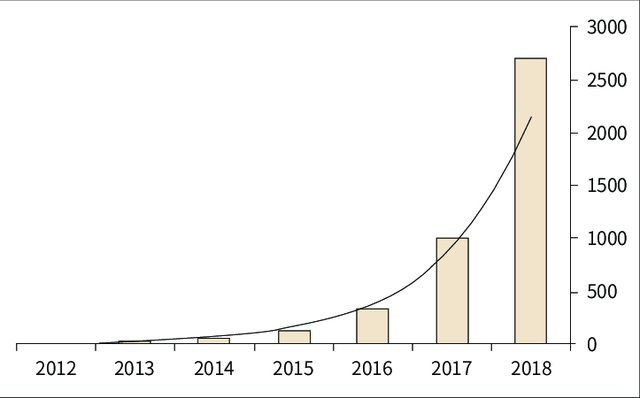
\includegraphics{img/Annual-trend-in-the-number-of-papers-related-to-deep-learning-in-the-medical-field_W640.jpg}
    \caption[Trend in publications about Deep Learning]{Trend in publications about Deep Learning  \cite{Number_of_DL_papers}}
    \label{fig:annual_trend}
\end{figure}


In such high-risk scenarios, DNNs should not only be highly accurate, as a mistake in detecting an obstacle could cause catastrophic consequences for the passengers, but also be trustworthy enough so that the probability of the predicted values reflects the ground truth. DNNs, however, are subjected to different source of uncertainty and errors. \textit{Galiwoski et al.} in \cite{gawlikowski2021survey} recognize five crucial factors which can cause uncertainty and errors in DNNs.\\\hfill

Those factors are:

\begin{enumerate}[label=\Roman*.]
    \item the variability in real world situations. 
    \item the errors inherent to the measurement systems,
    \item the errors in the architecture specification of the DNN,
    \item the errors in the training procedure of the DNN,
    \item the errors caused by unknown data.
\end{enumerate}
%In the next section, we will explore these factor in more details. Subsequently, we will reason about methods to reduce it and finally, in the third section, we will individuate methods to classify it. 
%\subsection{Factors causing Uncertainty}
We can model a neural network as a function $f$, parametrized by weight $\theta$, which maps a set of input $\mathbb{X}$ to a set of measurable outputs $\mathbb{Y}$, hence:
\begin{equation}
    f\theta : \mathbb{X} \rightarrow \mathbb{Y} \quad\quad\quad
    f\theta(x) = y
    \label{eq:DNN_model}
\end{equation}
In case of supervised learning, we also model the training set as $\mathcal{D} \subset \mathbb{D} = \mathbb{X} \times \mathbb{Y}$, where $\mathbb{X}$ is an instance space and $\mathbb{Y}$ the set of outcomes that can be associated with an instance (\cite{uncertainity_classi}), containing $N$ samples. A DNN trained in $\mathcal{D}$ can therefore predict a a corresponding target $f\theta(x^*) = y^*$.\\
During the data acquisition process, a measurement $x$ and a target variable $y$ are taken from space $\Omega$ to  represent a real world situation $\omega$. For example, $\omega$ could be a sugar beet, $y$ the label ''sugar beet'' and $x$ a picture of a sugar beet. The job of the DNN is therefore to predict the label from the image of the sugar beet (Eq n. \ref{eq:DNN_model}). In a real world situation, however, measurements could be potentially different from the ones used for training and this could influence the prediction of $y$. The source of this difference could be different lighting condition, different environmental condition or general conditions not taken into account when training.A new measurement generally is not part of the training set, hence $x^* \notin \mathcal{D}$.These differences in real world scenarios compared to the training set are called \textit{distribution shifts}(\cite{ovadia2019trust}) and DNN are very sensitive to that. Moreover, source of noise could also be individuated in errors in labelling. This is the first factor that can cause uncertainty, i.e. \textbf{the variability in real world situations}. \cite{gawlikowski2021survey}\\
In addition, it has to be taken into account that measurement devices are also subjected to noise due to defects or imprecision. This kind of noise is the second factor, i.e. \textbf{tthe errors inherent to the measurement systems}. \cite{gawlikowski2021survey}\\
We previously modelled a neural network simply as a function $f\theta$. Although in most applications DNN are treated similarly to how we modelled them, i.e. as a black box which takes as input some data and outputs a prediction, they have a certain structure with certain parameters to take care of. These parameters can be for example the amount of layer, the parameters which need to be configured and the chosen activation function. These configurations are up to the modeller and are the third cause of uncertainty in DNNs, i.e. \textbf{the errors in the architecture specification of the DNN}. \cite{gawlikowski2021survey}\\
A further source of uncertainty in DNNs is also related to the very own nature of DNNs. DNNs are not deterministic, rather they are stochastic\footnote{Stochastic is a synonym for randomness} in many ways : the order of data, the weight initialization or random regularization as augmentation or dropout. \cite{gawlikowski2021survey} Moreover, the stochastic gradient descent algorithm is widely use to optimize the learning process of DNNs. \cite{ruder2017overview}\\
Another version of the gradient descent algorithm which is also used is the mini-batch version, which selects random batches with aleatory size (called batch size) from the learning data-set to optimize the training process. \cite{ruder2017overview} This parameter, in addition to other ones like learning rate, and the number of training epochs, is also source of unpredictability in the DNN, as they could heavily change its performances  \\
The stochastic nature of DNN and the choices of the aforementioned parameters are the forth cause of uncertainty in DNNs : \textbf{the errors in the training procedure of the DNN}\\
Previously we modelled the training set as $\mathcal{D} \subset \mathbb{D}$, hence as being a subset of a certain domain $\mathbb{D}$. However, the realm of input which could be fed to a neural network is not limited to this domain, rather the DNN is trained to solve tasks with inputs belonging to this domain. Another source of uncertainty can be therefore an input which the DNN is not trained for, even though it is able to process it. For instance, if a DNN is trained to classify dogs from images, an image as input could also depict a bird. The last factor which could cause uncertainty is therefore the \textbf{errors caused by unknown data}. Such unknown data, could also be caused by highly noisy measurement devices, like a broken camera, and some researches show how easy is to fool DNN with images that are meaningless for us humans.\cite{nguyen2015deep} Fig n. \ref{fig:fooling_DNN} depicts some examples of picture which could fool even the most advanced DNN. The figures on the top row could also be produced by random noise from a malfunctioning camera and yet could be classified as something else with an accuracy $\geq$ 99.6\%. \cite{nguyen2015deep}\\
\begin{figure}[htb]
    \centering
    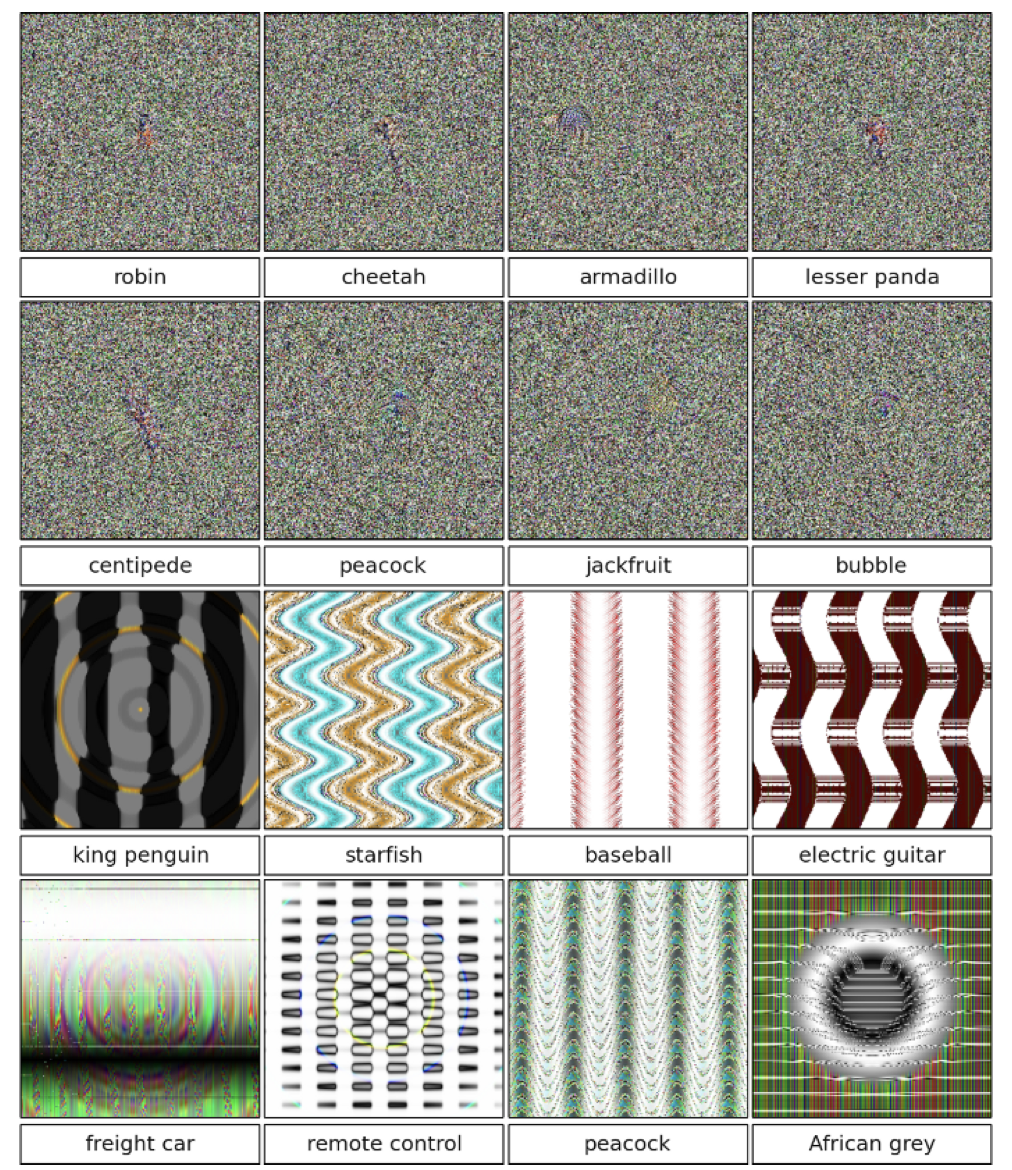
\includegraphics[scale = 0.4]{img/images_fooling_DNN.png}
    \caption[Differences between how DNNs and humans recognize objects]{This result highlights differences between how DNNs and humans recognize objects. Images are either directly (top) or indirectly (bottom) encoded \cite{nguyen2015deep}}
    \label{fig:fooling_DNN}
\end{figure}

With the help of the five factors we studied before, we can further categorize uncertainty in two main categories: aleatoric and epistemic uncertainty. \cite{Separation_uncer}

\begin{figure}[htb]
    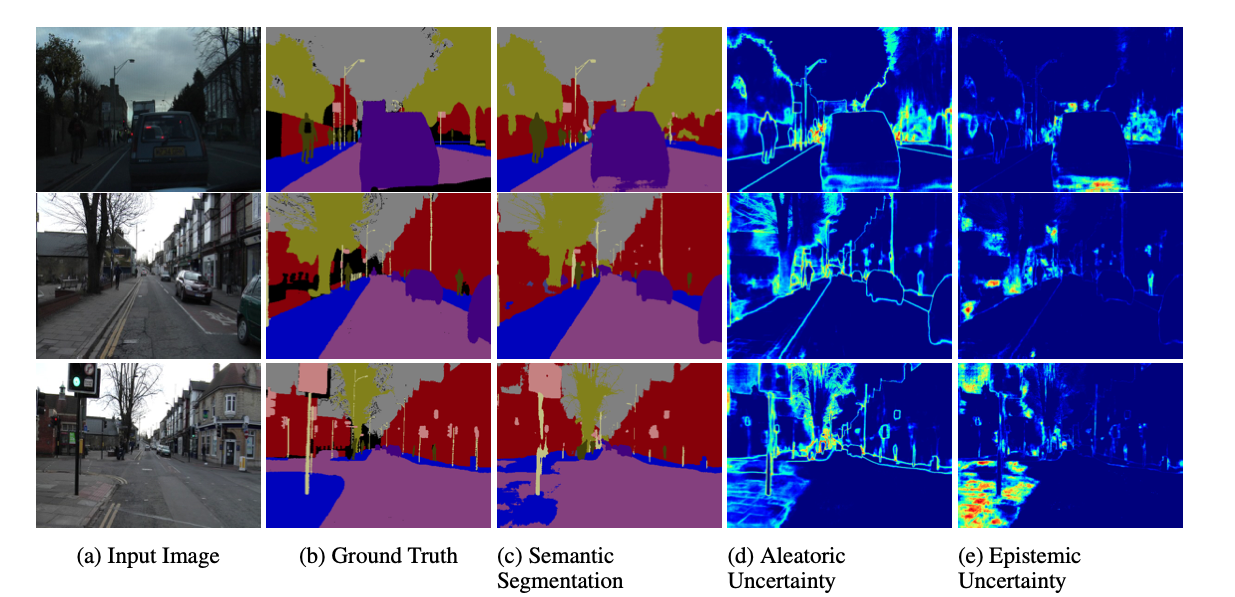
\includegraphics[scale = 0.4]{img/uncert_visua.png}
    \caption[Illustrating the difference between aleatoric and epistemic uncertainty]{Illustrating the difference between aleatoric and epistemic uncertainty for semantic segmentation on the CamVid dataset \cite{DBLP:journals/corr/abs-1811-01412}}
    \label{fig:un_visua}
\end{figure}




\textit{Aleatoric uncertainty} is also usually referred to as data or statistical uncertainty) and it is generally used to identify the type of uncertainty cause by the nature of randomness, that is \textit{ the variability in the outcome of an experiment which is due to inherently random effects} \cite{Separation_uncer}. Moreover, it also comprises the type of noise directly stemming from the noise in data used to train, validate, test and for inference, therefore referring to factor II \cite{gawlikowski2021survey} \cite{DBLP:journals/corr/abs-1811-01412}.  \\
Aleatoric uncertainty is of the irreducible type, meaning it is impossible to get rid of.(\cite{DBLP:journals/corr/KendallG17}, \cite{Separation_uncer}) For example, a model that predicts the output of a flip coin, even in case of a perfect model, is not able to produce the definite, correct answer for it, but only a prediction of the possibilities for the two outcomes. This is due to the fact that the data used for this model is of random, stochastic nature and this random component can not be reduced. \cite{Separation_uncer}\\
\textit{Epistemic uncertainty}, or systemic or epistemic uncertainty, on the other hand, refers to the type of uncertainty cause by ignorance or short comings of the model, hence not on any other underlying stochastic phenomenon. \cite{DBLP:journals/corr/abs-1811-01412}. Usually, this is due to unknown or lack of coverage of the dataset used for training, hence covers factors I,III, IV and V. \\
Epistemic uncertainty can be theoretically explained away by improving the architecture of the model and broadening the dataset.
For example,let us consider a model which is able to determine whether a word is part of the Italian or English dictionary. If we feed the word 'macchina'' to the model, given that we provided enough data to train and the model is perfect, we can be confident that it will predict the correct language, in this case Italian. However, if we feed it with the word ''pasta'', we can not be confident that the prediction is correct, i.e. we can only obtain the probability of this word to be part of one of the dictionaries \textbf{given the dataset we provided}. As a matter of fact, the word ''pasta'' is present in both dictionaries and the outcome depends on the probability of the word to appear in one of the dictionaries in our dataset. The first case is clear case of epistemic uncertainty, which we were able to completely remove with a perfect dataset; while the second case is a clear case of aleatoric uncertainty and it is impossible to remove. 
Fig n\ref{fig:un_visua} helps visualize the difference between the two. In pictures (\textit{d}), we can see that the aleatoric uncertainty increases on object boundaries and objects far from the camera. Pictures (\textit{e}), on the other hand, shows how epistemic uncertainty increases for semantically and visually challenging pixels. For example, the bottom row shows a failure case when the model fails to segment the footpath due to high epistemic uncertainty, but low aleatoric uncertainty. \cite{DBLP:journals/corr/KendallG17}\\
Although this distinction is very helpful for further and more precise analysis on a DNN model, it is also important to note that the distinction between the two is highly dependent on the context: they are not absolute notions.(\cite{KIUREGHIAN2009105}) Hence, changing the settings of the model will blur the distinction line between the two and therefore make their classification considerably more difficult.\cite{Separation_uncer}\\
We mentioned previously that theoretically model uncertainty is 100\% reducible. However, in case of real world data this is not the case. In addition to the probabilistic nature of the DNNs, the training dataset used for the model is very likely to be only a subset of all possible input data of the application, hence it is also very likely that unknown data for the domain is unavoidable. In addition, represent exactly the uncertainty of the DNN is not possible, as the different sources of uncertainty can not be generally modelled accurately. \cite{gawlikowski2021survey}\\

%\subsubsection{Modelling Uncertainty}
%\subsection{Classification of uncertainty}

%\subsection{Quantification of uncertainty}

%For a desired degree of confidence (namely, foir a given probability), a confidence interval is a prediction of the range of the output of a model where the actual value exists. With an assumption of a normal distribution of the errors, confidence intervals can be calculated for neural networks.\cite{Confidence_Interval}
%\subsection{Calibration of Neural Networks}
%\subsection{Final remarks on Uncertainty}


\section{Accuracy}\label{sec:accuracy}
Accuracy is usually one of the most looked after metrics when analysing Neural Network performances(\cite{hendrycks2019benchmarking},\cite{bianco2018dnnsbench}). Accuracy is usually the factor taken into account when the training process is evaluated, as could be a potential factor deciding when to stop it. Being able to predict accuracy, for example, could help detecting, and therefore terminate, unsuccessful training run \cite{unterthiner2021predicting}. \\
 Usually, the term ''accuracy''  refers to the \textit{classification accuracy} of the neural network. The classification accuracy is the ratio of the number of correct predictions to the total number of input sample (\cite{hussein}) and it is calculated with equation n. \ref{eq:cla_acc}.
\begin{equation}
Accuracy = \dfrac{Number\;of\;correct\;predictions}{Total\;number\;of\;predictions}
\label{eq:cla_acc}    
\end{equation}

In case of a multi-class prediction problem, however, classification accuracy is meaningful only when each class contains an equal number of samples. For example, considering two classes $A$ and $B$ containing 98\% and 2\% of the samples respectively, the model can reach 98\% accuracy by predicting exclusively samples from class $A$. \\
Another definition which is often used for accuracy in Neural Networks in the context of \textit{binary classification} is the one showed in equation n. \ref{eq:bin_acc}.
 \begin{equation}
Accuracy = \dfrac{TP+TN}{TP+TN+FP+FN}
\label{eq:bin_acc}    
\end{equation}
Where TP = True Positives, TN = True Negatives, FP = False Positives, and FN = False Negatives.\\
Similarly to classification accuracy, however, this definition could be misleading as well.  For example, considering a model that classified 100 tumors as malignant (the positive class) or benign (the negative class) as shown in Fig. n. \ref{fig:tumor}. 

\begin{figure}[h]
\centering
\begin{tabular}{ p{1cm} p{2cm} p{2cm} p{2cm}}
 TP&FP&FN&TN\\
 \hline
    1 & 1& 8& 90\\
\end{tabular}
\caption{Example for binary classification}
\label{fig:tumor}
\end{figure}
Calculating the accuracy using equation n. \ref{eq:bin_acc}. will give an accuracy of :
 \begin{equation}
Accuracy = \dfrac{1+90}{1+90+1+80} = 0.91
\label{eq:bin_acc2}    
  \end{equation}
At first glance, this metric would show that the model is performing correctly (91 correct out of a 100). The dataset is composed of 91 tumors that are benign (90 TNs and 1 FP) and 9 that are malignant (1 TP and 8 FNs). The model is able to identify 90 out of 91 benign tumors correctly, but only 1 out of 9 as malignant. This is another case of class-imbalanced data set in which a model that would only classify tumors as benign would reach the same level of accuracy. \cite{google_doc}\\



\section{Precision and Recall}
As we already delineated in the previous section, sometimes analysing only at accuracy might be misleading, especially when we are dealing with class-imbalanced data-sets. Accuracy does not distinguish between the number of correct labels of different classes. \cite{metrics}\\
In these cases, two other metrics we can observe are \textit{precision} and \textit{recall}. \\
Formally, \textit{precision} is defined as equation n. \ref{eq:pre} and it represents the number of detected anomalies that are actual real anomalies.\cite{tatbul2019precision}
In other words, it expresses the proportion of positive identifications that was correct. 
\begin{equation}
Precision = \dfrac{TP}{TP+FP}
\label{eq:pre}    
\end{equation}
Where TP = True Positives and FP = False Positives\\
On the other hand, \textit{recall} is defined as equation n. \ref{eq:rec} and it represents the number of real anomalies that have been detected.\cite{tatbul2019precision}
\begin{equation}
Recall = \dfrac{TP}{TP+FN}
\label{eq:rec}    
\end{equation}
Where TP = True Positives and FN = False Negatives\\

We can use the example in Fig. n . \ref{fig:tumor} to calculate both precision and recall. 
\begin{equation}
\begin{aligned}
Precision &= \dfrac{TP}{TP+FP}\\
          &= \dfrac{1}{1+1}\\
          &= \dfrac{1}{2}\\
          &= 0.5
\end{aligned}
\label{eq:pre_ex}    
\end{equation}
Having a precision of 0.5, our model is correct 50\% of the time when it predicts that a tumor is malignant. 
\begin{equation}
\begin{aligned}
Recall &= \dfrac{TP}{TP+FN}\\
          &= \dfrac{1}{1+8}\\
          &= \dfrac{1}{9}\\
          &= 0.11
\end{aligned}
\label{eq:rec2}    
\end{equation}
In other words, with a recall of 0.11, our model has been able to identify 11\% of all malignant tumors. \\
Ideally, we would like to have a high recall percentage as well as a high precision one. Unfortunately, this is rarely the case since improving recall often comes at the expense of precision, since in order to increase the TP for the minority class, the number of FP is also often increased, resulting in reduced precision. \cite{10.5555/2559492}\\
Furthermore, as it was the case for accuracy, neither precision nor recall give a full insight on the performance of the model, since a model could have high precision with low recall, as shown in the example above. It is, therefore, common practice to combine both with a weighted harmonic mean as an F score \cite{Rijsbergen1974FOUNDATIONOE}:
\begin{equation}
F_\beta = (1+ \beta ^2)\dfrac{Precision * Recall}{\beta ^2* Precision + Recall}
\label{eq:f_score}    
\end{equation}
In equation n. \ref{eq:f_score}, the coefficient $\beta$ represents the balance between Precision and Recall, with high values favouring Recall. Usually, the F-score is used with $\beta =1$, so a perfect balance between Precision and Recall, and in this case it is called F1 score(Equation n. \ref{eq:f1_score}). \cite{derczynski-2016-complementarity}
\begin{equation}
F1 = (2)\dfrac{Precision * Recall}{Precision + Recall}
\label{eq:f1_score}    
\end{equation}
When evaluating the F score, however,the focus is given exclusively to true positives, false positives and false negatives, neglecting the true negative group, which is usually the majority class. In addition, using the F score, one is unable to distinguish low-recall from low-precision systems. \cite{derczynski-2016-complementarity}\\
\section{Loss}
When training a Neural Network, finding the perfect weights for the neurons is impossible, therefore the problem is usually modelled as an optimization problem. As an optimization problem, it is solved using an algorithm which aims to optimize the weights to make good predictions. Usually, Neural Networks are trained using the Stochastic Gradient Descent (SGD) and the weights are updated through back-propagation. In the context of an optimization algorithm, the function which evaluates a candidate solution is defined as the objective function and such function in Neural Networks evaluates how good a prediction is, hence the SGD is used to minimize this function, i.e. finding the solution with the lowest score. 
When we are minimizing the objective function, we are referring to it as the cost function, loss function, or error function.\cite{Goodfellow-et-al-2016}\\
The loss function has the fundamental job of faithfully distill all the aspects of the model, both good and bad, down into a single, scalar value, which allows candidate solutions to be compared. \cite{reed_neural_1999}\\
The choice of the loss function is highly influenced by the output layer of the Neural Network. The output layer defines the type of the solution we defined for the problem, i.e. if it is a regression problem of a classification problem. In other words, the way we  represent the output determines the loss function. \cite{Goodfellow-et-al-2016}\\
The following are some of the best practices for each type of problem. 

\begin{description}
  \item[Regression problem] \hfill\\ 
  For these type of problems, usually the output layer is one node with a linear activation unit, therefore the loss function to use is the Mean Squared Error(MSE). 
  \item[Binary Classification problem] \hfill\\ 
  The output layer is one node with a sigmoid activation unit and the loss function used is Cross-Entropy, or Logarithmic loss. 
  \item[Multi-class Classification problem] \hfill\\ 
  The output layer is composed of one node for each class using the soft-max activation function nd the loss function used is Cross-Entropy, or Logarithmic loss. 
\end{description}


%\cite{10.5555/525960}



%\url{https://machinelearningmastery.com/loss-and-loss-functions-for-training-deep-learning-neural-networks/}

\section{Over-fitting and Under-fitting }\label{sec:of_uf}
As we already discovered in section n. \ref{sec:training_time}, the training routine is necessary for the model in order to make predictions on a new set of data. Therefore, the goal of the learning process is not to minimize the accuracy on the training set, but rather to maximize its predictive accuracy on the new data points. \citep{dietterich1995overfitting}\\
If the model works too hard to find the best fit for the training data there is the risk that it is going to fit the noise present on the data-set, hence it will learn the inevitable peculiarities and bias present in the training set, rather than finding a general predictive rule. In other words, the performance of the model will decrease when tested against an unknown data-set.\cite{jabbar2015methods} This phenomena is called \textit{over-fitting}. \citep{dietterich1995overfitting}\\
Over-fitting is influenced by the training data fed to the model, as small data-sets are more prone to it, even though also large data-sets can be affected. \cite{10.1016/j.inffus.2008.11.003}\\
Under-fitting, on the other hand, can be considered as the opposite process. This occurs when the model is too simple for the training data and it is incapable of learning the variability of the data. \cite{10.1016/j.inffus.2008.11.003}\\

One strategy to avoid over-fitting is to use a so-called ''early-stopping'' approach. This approach consists simply of stopping the training before over-fitting can occur and it is one of the mostly used strategies to avoid this phenomena, as it is simple to understand and proven to be the superior one in many cases (\citep{FINNOFF1993771}, \cite{early_stopping}). \\
The key part of this approach is to divide the training set into two parts, namely the validation set and the training set, and to use those to find a criteria to stop the training process. \\
Fig. n. \ref{fig:over_fitting_curve} shows the idealized evolution over time of the error on the training set and on a validation set not used for training, i.e. training and validation loss.\cite{early_stopping}

\begin{figure}[htb]
    \centering
    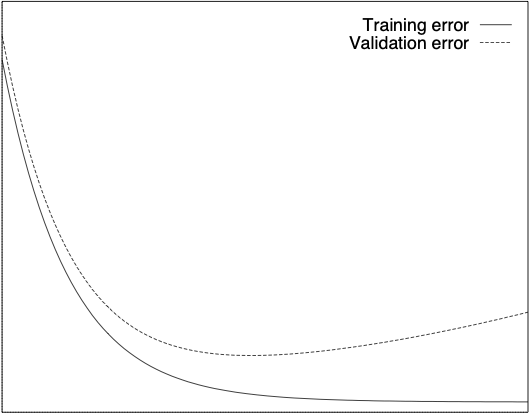
\includegraphics[scale = 0.3]{img/over_fitting.png}
    \caption[Validation and training loss curve]{Validation and training loss curve. The x axis is time, the y axis is the loss \cite{early_stopping}}
    \label{fig:over_fitting_curve}
\end{figure}


Following the trend in Fig. n. \ref{fig:over_fitting_curve}, we can observe that the validation error decreases until a certain point together with the training loss before increasing indefinitely. We can use the validation error to approximate the generalization error and, therefore, stop the training in the moment where the validation loss is increasing again. 
We can summarize the ''early-stopping'' approach in the following steps:
\begin{enumerate}
\item Split the training data into a training set and a validation set, for i.g. in a 4-to-1 proportion
\item Train over the training and evaluate the validation loss every arbitrary number of epoch
\item Stop training as so on as the error on the validation set is         higher than it was last time
\item Use the weights the network had in that previous step as the result of the training run

\end{enumerate}
Furthermore, depending on the data, there might be also situations in which the validation loss is not constantly bigger than the training loss, as shown in Fig. n. \ref{fig:over_fitting_curve}. As a matter of fact, this graph shows an idealized behaviour of the two curves. A real example for this curve can be seen in Fig. n. \ref{fig:over_fitting_curve_real}.
\begin{figure}[htb]
    \centering
    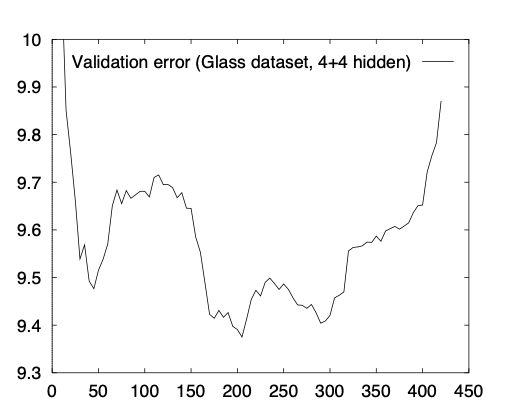
\includegraphics[scale = 0.4]{img/over_fitting_real.png}
    \caption[Real Example of the Validation and training loss curve]{Real Example of the Validation and training loss curve. The x axis is time, the y axis is the loss \cite{early_stopping}}
    \label{fig:over_fitting_curve_real}
\end{figure}

In such situations, it would be particularly difficult to choose an optimal stopping criteria, as the validation function as multiple local minima (16 in the pictures case). It is left to the reader to investigate strategies to optimize early-stopping in these situations. \\
Furthermore, there are also scenarios in which, depending on the data presented, the validation loss is at first less than the training loss, as shown in Fig. n. \ref{fig:over_fitting_curve_2}. 
\begin{figure}[htb]
    \centering
    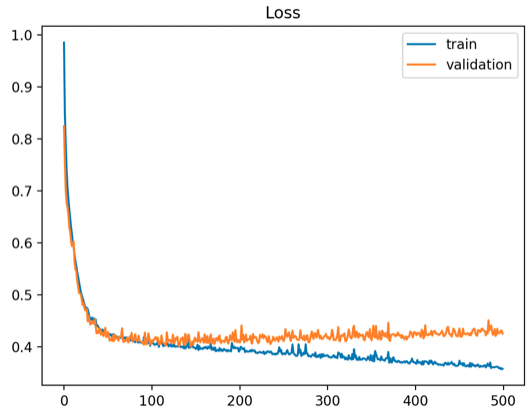
\includegraphics[scale = 0.4]{img/over_fitting_2.png}
    \caption[Real Example of the Validation and training loss curve]{Real Example of Validation and training loss curve. The x axis is time, the y axis is the loss}
    \label{fig:over_fitting_curve_2}
\end{figure}

In these situation, as a rule of thumb, we can use the following statements to determine the status of the training and decide when to stop. 
\begin{itemize}
\item validation loss $>>$ training loss: over-fitting
\item validation loss $>$ training loss: some over-fitting
\item validation loss $<$ training loss: some under-fitting
\item validation loss $<<$ training loss: under-fitting

\end{itemize}


\section{Architecture}\label{sec:arch}
In the following sections we are going to briefly analyse the architectures of the models we are going to study to find characteristics and correlations. \\
For the sake of this paper, we are going to limit our analysis to some of the most common architectures for convolutional neural networks which have been proven by other studies (\cite{suh_transfer_2018}, \cite{s20205893}, \cite{phdthesis}) to achieve promising results in the settings of sugar beet recognition. The architecture chosen are listed below and are treated in more details in their respective sections. 
\begin{itemize}
\item Resnet
\item Alexnet
\item VGG
\end{itemize}
\subsection{Alexnet}
Alexnet is a Convolutional Neural Network (CNN) architecture designed by  Alex Krizhevsky in collaboration with Ilya Sutskever and Geoffrey Hinton. \cite{NIPS2012_c399862d}\\
The architecture is depicted in Fig. n. \ref{fig:alexnet_architecture}. The net is composed of eight layers:
The first 5 are convolutional layer an convolutional and the remaining three are fully- connected. The output of the last fully-connected layer is fed to a 1000-way Softmax which produces a distribution over the 1000 class labels. \cite{NIPS2012_c399862d}\\
\begin{figure}[htb]
    \centering
    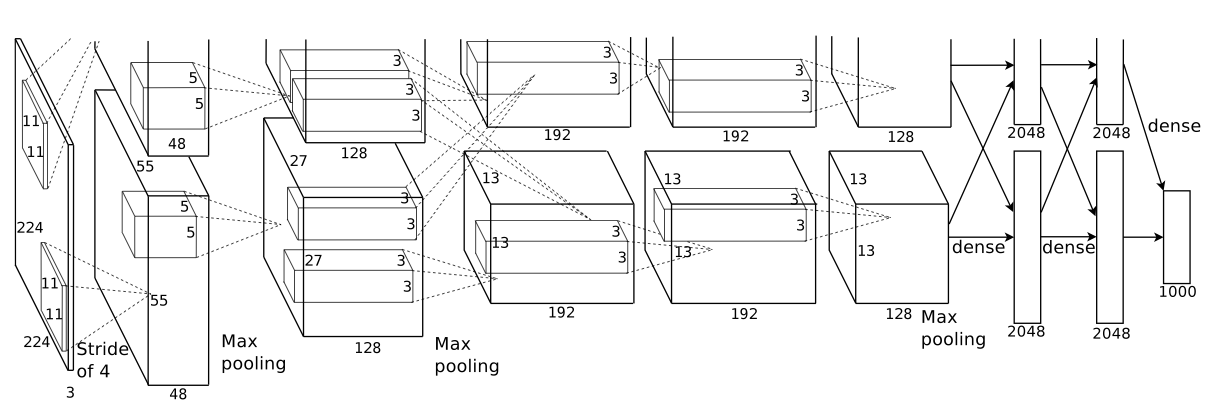
\includegraphics[scale = 0.4]{img/alexnet_architecture.png}
    \caption[Overview of the architecture of Alexnet]{Overview of the architecture of Alexnet \cite{NIPS2012_c399862d}}
    \label{fig:alexnet_architecture}
\end{figure}


As described by \textit{Krizhevsky et al.} in \cite{NIPS2012_c399862d}, the layers are defined as it follows:

\begin{itemize}
\item The first convolutional layer receive as input a 224 × 224 × 3  image and filters it with 96 kernels of size 11 × 11 × 3 with a stride of 4 pixels\footnote{The stride is the distance between the receptive field centers of neighboring neurons in a kernel map}
\item The second convolutional layer takes as input the response-normalized and pooled output of the first layer and filters it with 256 kernels of size 5 × 5 × 48.
\item The third layer has 384 kernels of size 3 × 3 × 256 it is connected to the normalized and pooled output of the second
\item The fourth convolutional layer has 384 kernels of size 3 × 3 × 192 and it is connected to the third without pooling or normalization layers
\item The fifth convolutional layer has 256 kernels of size 3 × 3 × 192 and as input it receives the output of the forth. 
\item The fully-connected layers are composed of 4096 neurons each
\end{itemize}
\subsection{VGG Networks}\label{sec:VGG}
VGG stands for Visual Geometry Group at Oxford University and have been developed by Simonyan and Zisserman in \cite{simonyan2015deep} for the 
ILSVRC (Image Net Large Scale Visual Recognition Challenge) 2014 competition
(\cite{DBLP:journals/corr/RussakovskyDSKSMHKKBBF14}). 
The concept of VGG net is similar to Alexnet: as net increases, the number of convolutions and future maps increases as well. Rather than using 11 × 11 feature detectors or filters, however, the authors decided to use smaller 3 x 3  filters. The various architecture proposed in \cite{simonyan2015deep} are showed in Fig. n. \ref{fig:vgg_arch}. In this paper, we are going to consider only the networks D and E, i.e. with 16 and 19 weight layers respectively. For the rest of the paper, we are going to refer to them as VGG16 and VGG19 respectively. 

\begin{figure}[htb]
    \centering
    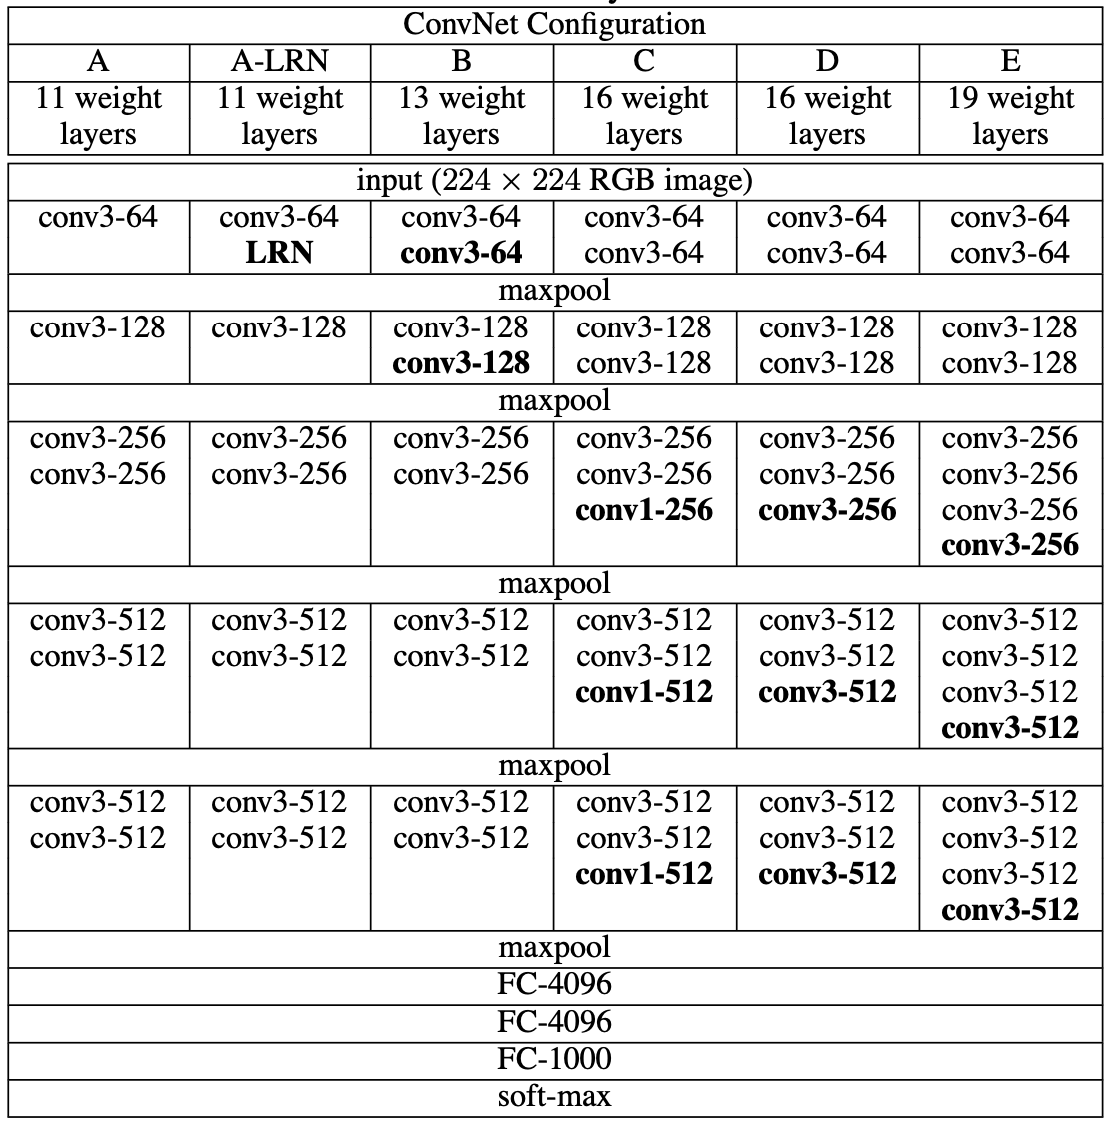
\includegraphics[scale = 0.5]{img/vgg_arch.png}
    \caption[Overview of the various architecture for VGG]{Overview of the various architecture for VGG \cite{simonyan2015deep}}
    \label{fig:vgg_arch}
\end{figure}



%\begin{figure}[htb]
 %   \centering
  %  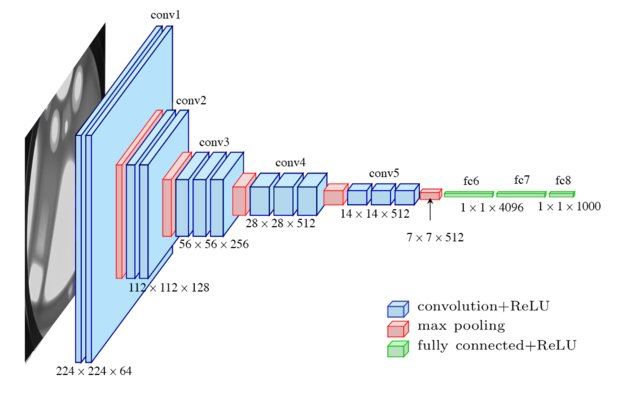
\includegraphics[scale = 0.5]{img/vgg_picture.jpg}
   % \caption[Residual learning: a building block]{\cite{vgg_picture}}
  %  \label{fig:res_block}
%\end{figure}





\subsection[Residual Neural Networks]{Residual Neural Networks (Resnet)}
Many studies (\citep{simonyan2015deep}, \cite{szegedy2014going}) reveal that the depth of the Neural Networks is crucial and for most visual recognition tasks the trend has been to stack more layers into neural networks and increase their depth. (\cite{simonyan2015deep},\cite{ioffe2015batch},\cite{girshick2014rich},\cite{2014Spatial})\\
Training deeper networks like VGG19 and VGG16 (section n.\ref{sec:VGG} ), however, is not a trivial task, since,as they start converging, the accuracy starts to saturate and then degrades quickly. This phenomena is due to the gradient vanishing during back-propagation, i.e. when the weights are updated, as it becomes smaller the more layers it goes through and vanishes before reaching the initial layer, hence they can not be updated.  \\
\textit{He et al. } in \cite{DBLP:journals/corr/HeZRS15} tackle the problem of degradation with the introduction of a \textit{deep residual learning} framework. At the core of the framework there is the so called ''residual block'', shown in Fig. n. \ref{fig:res_block}. 
\begin{figure}[htb]
    \centering
    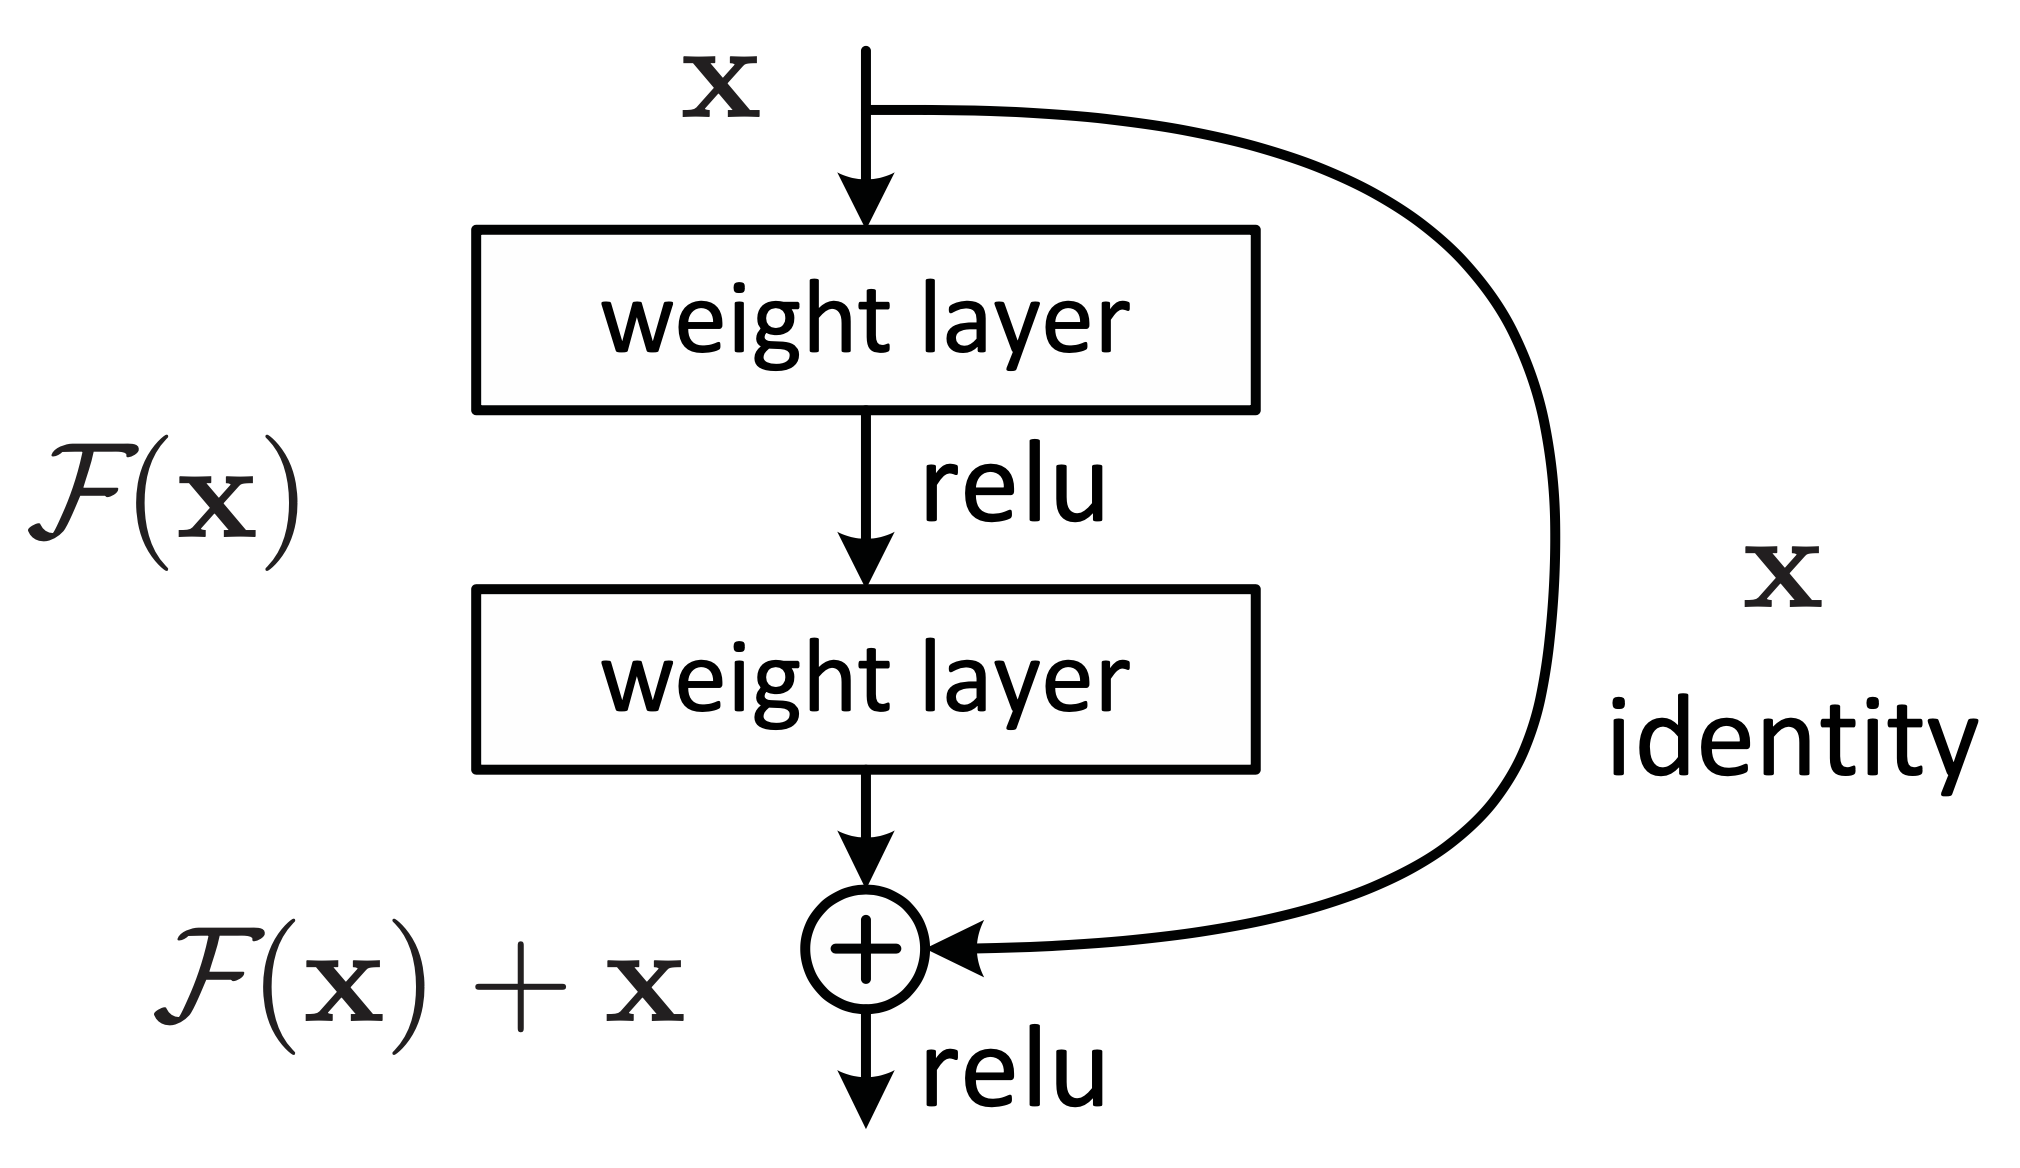
\includegraphics[scale = 0.3]{img/res_block.png}
    \caption[Residual learning: a building block]{Residual learning: a building block. \cite{DBLP:journals/corr/HeZRS15}}
    \label{fig:res_block}
\end{figure}

Differently from plain convolutional networks, these blocks also have the so called ''identity connection'' between the input and the output layer. 
In plain convolutional networks, the output $\mathcal{H}(x)$ is obtained by:
\begin{align*}
\mathcal{H}(x) &= \mathcal{F}(wx + b)\\
               &or\\
\mathcal{H}(x) &= \mathcal{F}(x)\\   
\end{align*}
with $w$ being the weights and $b$ being the bias\\
With the introduction of residual blocks, the output function assumes the form showed in equation n. \ref{eq:residual_blocks}.
\begin{equation}
\mathcal{H}(x) = \mathcal{F}(x) + x
\label{eq:residual_blocks}   
\end{equation}
Reworking the equation lets us obtain the so called \textit{residual function}: 
\begin{equation}
\mathcal{F}(x) = \mathcal{H}(x) - x
\label{eq:residual_function}   
\end{equation}

The purpose of residual networks becomes to approximate the residual function, hence the difference between the input and the output.In other words, the aim is to learn the residual function in a way such that it approaches zero, hence making the identity value optimal. \\
The problem of the vanishing gradient is resolved by the identity function. During back-propagation the gradient can take this path and, since no weights are encountered, there won't be any change in the value computed by the gradient. This effectively allows the gradient to entirely skip the block and reach the initial layers and correct their weights. \\
The architecture of residual networks we are going to use in this paper is showed in Fig. n. \ref{fig:resnet_arch}. For the rest of the paper, we are going to refer them as ''Resnet'' followed by the amount of layers. For example, Resnet18 refers to the residual network having the 18 layers described in Fig. n.  \ref{fig:resnet_arch}. 
\begin{figure}[t]
    \centering
    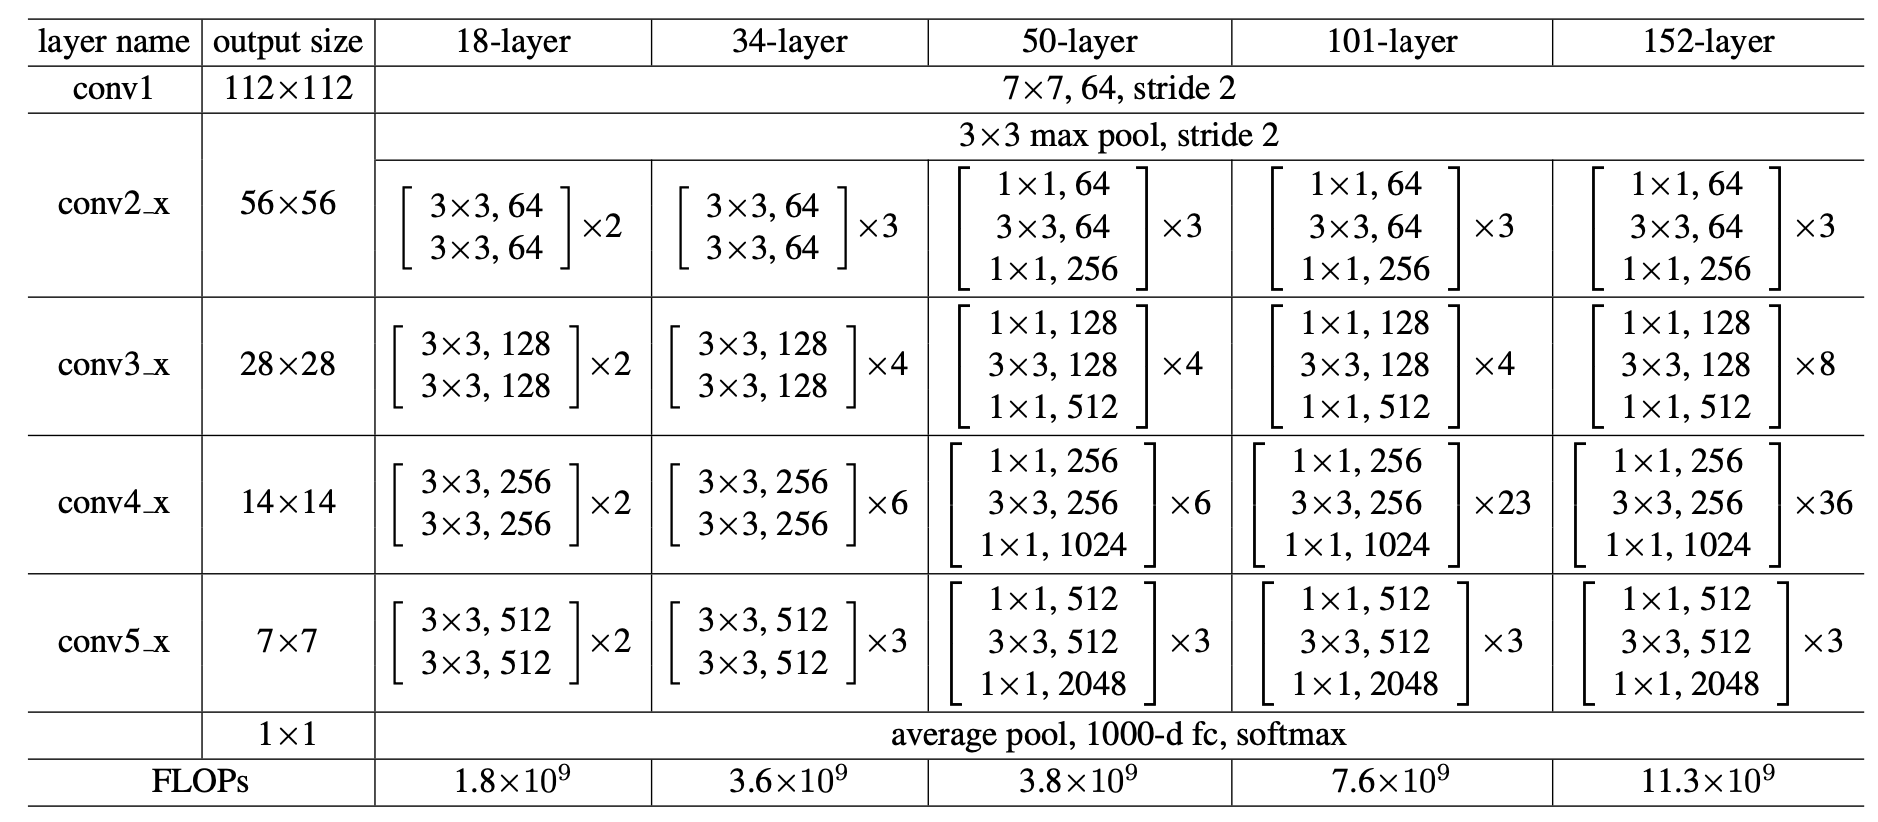
\includegraphics[scale = 0.5]{img/resnet_arch.png}
    \caption[Overview of the Resnet Architecture]{Overview of the Resnet Architecture. The building blocks are shown in brackets \cite{DBLP:journals/corr/HeZRS15}}
    \label{fig:resnet_arch}
\end{figure}



\chapter{Analysing the models}\label{ana_models}
\section{Introduction}

Before discussing how to use the characteristics of a model to optimize complex application, it is vital we find a way to measure and evaluate models. As the whole application will have its foundations on those measurements, finding them precisely and reliably is our main goal. Moreover, we are expecting applications to be composed of devices with completely different characteristics, both in hardware and software. Although it is possible to predict some of the characteristics of NNs using their weights (\cite{Unterthiner2020PredictingNN}), in this paper we will rely upon methods to find the empirically. The output of our investigation will be a toolbox which we can easily run on any device to measure the characteristics we are mostly interested in. \\
In section \ref{benchmarking} we will explore benchmarking in general terms to make an idea of benchmarks and to develop the requirements we will need to full-fill. In section \ref{benchmarking_nn} we will dive deep into measuring NNs' performances and to find the tools we can use for our own benchmark. Finally, in section \ref{sec:my_bench} we will describe the benchmark and we will use it to measure the performances of some networks. 

\section{Benchmarking}\label{benchmarking}
Benchmarking is a widely used tool to evaluate the performance of a system, either software or hardware, whose main goal is to produce consistent and precise measurements of said systems. High precision and affidabilty in benchmarks, however, have been always tricky to achieve and the complexity of these tasks have reached a high complexity in later years, due to advanced processor designs and very intricate interaction between programs and operating systems.\cite{DBLP:journals/corr/abs-1811-01412}\\
In addition, knowledge about the timing behavior of tasks, more specifically their worst-case execution times (WCETs) , is of the highest importance for building reliable and dependable real-time systems.\cite{Real-Time-Systems}\\
According to \textit{von Kistowski et al.} in \cite{how_to_bench}, benchmarks should follow certain key characteristics in order to be reliable:

\begin{itemize}
    \item Relevance
    \item Reproducibility
    \item Fairness
    \item Verifiability
    \item Usability
\end{itemize}
In the next section, we will better define them and describe them thoroughly. Understanding these characteristics is essential to produce precise and reliable measurements. Subsequently, we will explore some common techniques used to benchmark software. In section \ref{sec:remove_inter}, some of the main roadblocks and pitfalls of benchmarks are described to help the reader avoid them. In the same section, we will also point out some strategies to reduce measurement noise. Finally, in section \ref{sec:my_bench}, the benchmark used in this paper is described to facilitate its reproducibility. \\









\subsection{Key characteristics for a correct benchmark}\label{key_char}
In this section, we will explore the main characteristics a benchmark should possess in order to be a good benchmark.
\subsubsection{Relevance}
Relevance is probably the most important criteria. Relevance measures how close the behavior of the benchmark relates to the behaviors it is trying to test. \cite{how_to_bench}\\
Even if the benchmark is realized perfectly and respects all the other characteristics, if the results do not provide relevant information they are of no use. It is when the relevance of the benchmark is taken into account that the computer scientists or engineers need to make the first trade-offs and the first considerations. As a matter of fact, benchmarks that are designed to be highly relevant in a specific scenario tend to have a narrow applicability; vice-versa, benchmarks with a broader spectrum are usually less indicative in specific scenarios. \cite{how_to_bench}\\
Relevance also relates to the scalability of the benchmark. For example, benchmarks designed to test the full ability of servers might use the full resources that the server offers, for i.e. multi-threading, therefore will not perform correctly in system that do not have this possibility. \cite{how_to_bench}

\subsubsection{Reproducibility}
Reproducibility is the ability to consistently obtain similar, if not equivalent, results if the benchmark is tested on the same environment. \cite{how_to_bench}\\
Reproducibility is tightly correlated to the ability of describing the environment in perfect details, so that it could be performed on the same environment and expect similar results. The hardware must be described perfectly and software versions must be included and documented, as well as every other configuration done on the system. Especially with the increase of complexity in modern hardware architecture and modern operating systems, variability in performance is introduced by several actor, including  timing of thread scheduling, physical disk layout and  user interaction. \cite{how_to_bench}\\
Such variability can be addressed by running the benchmark for long enough periods of time in steady state, therefore without factors like user interaction. 


\subsubsection{Fairness}
In order to create a perfect benchmark, fairness is a characteristic that should be taken into account. A fair benchmark is a benchmark that allow the results obtained in different systems with completely different hardware and software to be comparable. Benchmarks are simplistic and, by their own nature, include a certain degree of artificiality, so it is necessary to put some constrains in order to stop the programs to "exploit" them. Those restrictions can be put, for example, in the software used.\\ 
\textit{Kistowski et al.} in \cite{how_to_bench} point out, for example, a benchmark realized in Java requires a virtual machine on top of the operating systems and the choice of virtual machine can heavily influence the results. This shows how limiting software and hardware components must be carefully limited to insure fairness in the results. However, putting too many limitations may actually hide some of the results, which might be relevant. \cite{how_to_bench} Therefore it is essential to find a good balance amongst the different limitations. \\
Furthermore, portability plays also a huge role in a fair benchmark. If too many limitations are imposed, or if those limitations are too strict, a big pool of devices could be not suitable to run the benchmark. Similarly to the amount of limitations, portability is also a factor which requires a trade off. As a matter of fact, the portability of a benchmark strictly depends on the very nature of the devices which are set to be used. 

\subsubsection{Verifiability}
A good benchmark should be able to provide trustworthy results and also results whose trustworthiness can be verified. To ensure the verifiability of the results, good benchmark usually run some self-verification tasks during run-time, for i.e. if hyper-threading is still active when it should not. Moreover, it is also the case that some benchmarks let users configure some parameters. Those configurations should be documented, as an undocumented alteration might define the result as not trustworthy. \cite{how_to_bench}
Finally, it is also good practice to include more metrics in the results as the ones strictly needed, since some red flags might be raised by inconsistencies in these metrics. 
\subsubsection{Usability}
Usability is the characteristics of a benchmark which aims to remove roadblocks for users to run the benchmark in their environments. This feature is not limited to how easy is to run the benchmark,which should be high, but some of the aforementioned characteristics relate to this one. For example, a good description of the benchmark also improves the usability of it, since it is easier to replicate. In addition, if the benchmark is too complex or expensive for its purpose might limit a potential user and not allowing them to effectively reproduce the tests. 



\subsection{Benchmark Techniques and Methodologies}\label{BTaM}

This section will delineate the different methodologies to measure the execution time of programs. It will contain techniques for both the \textit{wall time} and the \textit{CPU time}. \\
We are going to use the term  \textit{CPU time} to define the time spent by the CPU to process a piece of software, while we are going to use the term \textit{Wall Time} to indicate the time elapsed between the start and the end of the execution of a program.\\\hfill
Measuring the wall time of a program is the most straightforward, as it can also be done analogically using a manual stopwatch: simply start the time as the program starts and stop it as the program finishes. This method is undoubtedly imprecise and not very flexible, as it can only be applied to program whose needed measurements are just rough approximation.\cite{Stewart2001MeasuringET}\\
The equivalent method in UNIX-like systems is by using the command \textit{date}, which returns the system date and time. Due to the imprecise nature of such method it will not be described further. \\
A method along the lines of the one described above is by using functions like \textit{clock()} within the program we are trying to benchmark. This function needs to be used within the code of the program, similarly to the snippet of code n.\ref{fig:code} \cite{Stewart2001MeasuringET}, therefore it is limited to measure only small parts of the program. \\
\begin{figure}
\begin{lstlisting}[language=C, label= code]
    #include <time.h>
    
    //...
    
    clock_t start,finish;
    double total;
    start = clock();
    // Insert function here
    finish = clock();
    total = (double) (finish - start) / (double) CLK_TCK
    printf("Total = %f\n",total);
    
\end{lstlisting}
\caption{Example of use for the function \textit{clock()}}
\label{fig:code}
\end{figure}
In addition, such functions present two other problems. Since the function does not have a standardized implementation, the result may vary from device to device, which makes reproducibility impossible. 
Furthermore, these type of function needs to be executed as well, similarly to any other function in the code, hence they might introduce overhead and noise in the measurements. \\

A better way to measure the \textit{wall time} of a program is to use the UNIX command \textit{time}. The synopsis for this program is the following: \cite{linux_commands}\\
\begin{figure*}[h]
\begin{lstlisting}[language=bash]
   $ time [options] command [arguments...]
\end{lstlisting}
\caption{Synopsis of the command \textit{time}}
\label{fig:time_code}
\end{figure*}
The \textit{time} command runs the specified \textbf{command}, which can be running a specific program, and, as the program finishes, it returns the giving timing statistics about this program run.
These statistic consist of \textit{(i)} the elapsed real time between start and end of the program, hence the wall time, defined as \textbf{real}; \textit{(ii)} the CPU time, excluding I/O blocking functions, time for preemption and the time used for other OS related functions, defined as \textbf{user}, or user time;\textit{(iii)} and the time spent by the OS to execute tasks on behalf of the user, defined as \textbf{sys}, or system time. The last one includes time for preemption and I/O blocking functions, or any other function associated to the program. \cite{Stewart2001MeasuringET}
It is worth to note that some shells have a built-in \textit{time} command, hence may vary from the original one. To access the real one, it is suggested to specify its path-name (for i.g. /usr/bin/time).\cite{linux_commands} 

Nevertheless, we can run a small C++ program to give an example of how to use this command and to analyze its output. The snippet of the code can be seen in Fig n.\ref{fig:time_code_cpp}. The program we are going to use simply accumulates numbers from 0  to 10000000000 and prints the result on screen. Before we start accumulating, however, we add a small delay, namely 1 second, to check if this will be counted in the CPU time. Once the code has been compiled, we can run it as shown in Fig n. \ref{fig:time_code}, hence by writing \textit{time ./accumulate} in the shell \footnote{''accumulate'' is the name of the program and we assume to be in the correct directory}.\\
From the result we can observe the three indications of time we described earlier (user, system and total time).  In the case of the machine used for this paper, the user time was roughly 24,11 seconds, the user time roughly 0,05 seconds and the total time 25,254 seconds. \\
From these measurements, we can clearly observe that the total time is around one second bigger than the user time and the system time combined and it is due to the delay we introduced in line 6. If we comment out this line and we run the test once again, the total time now roughly equalizes the combination of user and system time (23,46s user 0,03s system, 23,578 total)


\begin{figure*}[h]
\begin{lstlisting}[language=c]
    #include <iostream>
    #include <chrono>
    #include <thread>
    
    int main(){
        std::this_thread::sleep_for(std::chrono::milliseconds(1000));
        double accumulate = 0 ;
        for(double i= 0; i< 10000000000; i++)
            accumulate += i;
        std::cout << "Result : "<< accumulate <<std::endl;  
        return 0;
    }
\end{lstlisting}
\caption{Program used to test the command \textit{time}}
\label{fig:time_code_cpp}
\end{figure*}


Even though the \textit{time} command offers multiple information, the time calculated and showed might not be reliable. As pointed out by \textit{Beyer et al.} in \cite{Beyer2017ReliableBR}, this command does not reliable include the CPU time of child processes. This is due to the fact that the Linux kernel is able to count the CPU time of a child process if that process terminated before the parent and the parent waited for it. If this happens, the CPU time of the child is lost and this will interfere with the precision of the measurements.\cite{Beyer2017ReliableBR},\\ \hfill

\textit{Beyer et al.} in \cite{Beyer2017ReliableBR} introduces also another another tool for benchmarks in their solution: control groups (cgroups). The Linux manual defines cgroups as "a Linux kernel feature which allow processes to be organized into hierarchical groups whose usage of various types of resources can then be limited and monitored". \cite{LinuxManualWeb} Cgroups therefore allow the user to assign processes to a group and every child process spawned by the assigned process will be tracked down. \\
Cgroups have been initially release with Linux 2.6.24, however, due to the problems with the initial version, starting from Linux 3.10, cgroups version2 have been introduced. In this paper, we will not describe the differences between the two versions, as it is not the purpose of this paper (we refer to the Linux manual for further details \footnote{ \url{https://man7.org/linux/man-pages/man7/cgroups.7.html}}) and the \textit{controllers} we are interested in did not change in functionality.  \textit{Controllers} allow the user to easily control and measure a specific resource within each group. \cite{Beyer2017ReliableBR}\\
The following \textit{controllers} are the ones we are more interested in:
\begin{itemize}
    \item[] \textbf{cpu} \quad    can guarantee a minimum number of CPU resource, even when the system is busy. However, this does not limit the CPU use in case of a free CPU
    \item[] \textbf{cpuacct} \quad provides information about the accomulated CPU usage
    \item[] \textbf{cpuset} \quad restrics the number of CPU cores available to a cgroup. In a system with more than one CPU and nonuniform memory access (NUMA) it allows to restric also the process to a subset of the physical memory  \cite{Beyer2017ReliableBR}
    \item[] \textbf{freezer} \quad allows to suspend and resume all processes in the group
    \item[] \textbf{pids} \quad allows to limit the number of spawnable processes. 
\end{itemize}
In addition to a more precise calculation of the CPU time, \textit{cgroups} augment also the fairness and the verifiability of the benchmark. By limiting the resources of a more powerful machine, the benchmark can have similar results to a much less powerful one, hence increasing fairness. 
Although this approach may hinder usability, as it is more cumbersome to set up than using the \textit{time} command, the benefits in precision make this trade-off worth it. 
\subsection{Common Practices in benchmarking}\label{sec:ben_challenges} \label{sec:remove_inter}
In section \ref{BTaM} we already discussed some of the issues which can be encountered when trying to design benchmarks. The pitfalls however are not limited to those challenges; on the contrary, it is notoriously difficult to obtain consistent results when designing benchmarks. In this section, we will explore some techniques to effectively reduce the non-determinism of lots of features, both hardware and software, which intend to increase performances. In most cases, since we have little to no control over them, the solution will be to disable these features. Although it will effectively get rid of the non-determinism, the environment we are going to create does not reflect how the application will run on a real application, however it would allow us to obtain consistent results. \\
The first element we are going to analyse is Turbo-boost. This feature will automatically make the processor core run faster than the marked frequency. \textit{Acun et al.} in \cite{turbo_boost} calculated an execution time difference of up to 16\% amongst processors on the Turbo Boost-enabled supercomputers. Since we have little control over it, the only solution to limit this variation is to completely disable it. The commands to permanently disable it are shoun in Fig. n. \ref{fig:no_boos}
\begin{figure}[h]
\begin{lstlisting}[language=bash]
# Intel
echo 1 > /sys/devices/system/cpu/intel_pstate/no_turbo
# AMD
echo 0 > /sys/devices/system/cpu/cpufreq/boost
\end{lstlisting}
\caption{Disable turbo boost in both AMD and Intel devices}
\label{fig:no_boos}
\end{figure}

Modern CPUs often employ a technique called Simultaneous multi-threading (SMT) to speed up execution. This technique makes it possible for two threads run simultaneously on the same core sharing execution resources like the cache or ALU.In case of Intel processor, the implementation of this technology is called Hyper-threading.\\
As a result of this implementation, it might happen that the sibling thread steals cache space for example from the workload we want to measure. To avoid these situations and limit the number of CPU-migrations, we will need to disable Hyper-threading by turning down the sibling thread in each core as shown in Fig. n. \ref{fig:no_ht}. 
\begin{figure}[h]
\begin{lstlisting}[language=bash]
# X being the CPU number
echo 0 > /sys/devices/system/cpu/cpuX/online
# To check the pair of CPU x
/sys/devices/system/cpu/cpuX/topology/thread_siblings_list
\end{lstlisting}
\caption{Disable Hyper-Threading}
\label{fig:no_ht}
\end{figure}

Another technique we can use to reduce noise in our measurements is  to bind a process to a certain CPU core. In Linux we can do that with the \textit{taskset} tool. \cite{LinuxManualWeb}\\
Furthermore, we can also increase the process priority with the command \textit{nice}. Processes with higher priority will get more CPU time since the Linux scheduler will favour them compared to processes with normal priority of 10. \cite{LinuxManualWeb}\\
A further step to take is to set the scaling governor policy to be \textit{performance}. The scaling governor changes the clock speed of the CPUs on the fly to save battery power, because the lower the clock speed, the less power the CPU consumes. To set the policy to be \textit{performance} one can use the method described in Fig. n. \ref{fig:per_sca}
\begin{figure}[h]
\begin{lstlisting}[language=bash]
for i in /sys/devices/system/cpu/cpu*/cpufreq/scaling_governor
do
  echo performance > $i
done
\end{lstlisting}
\caption{Set the scaling governor policy to be \textit{performance} for every cpu}
\label{fig:per_sca}
\end{figure}



\section{Benchmarking Deep Neural Networks}\label{benchmarking_nn}
Once we understood benchmarks and the characteristics they should possess, we can explore more deeply how we can benchmark Deep Neural Network(DNN).\\
As expressed by \textit{Reddi et al. } in \cite{reddi2020mlperf}, ''Designing ML benchmarks is different from designing traditional non-ML benchmarks''. As a matter of fact, the spectrum of tasks NNs can perform is very broad, consequently there is a wide spectrum of requirements they need to fulfil, making the development of a reliable and relevant benchmark, which is at the same time universal, untreatable. In this paper, we are interested in measuring performances in images classification tasks in the settings of sugar beet recognition. Moreover, although, benchmarks are usually designed to compare performances, the scope of our investigation is to precisely measure the characteristics of Neural Networks and to find possible correlations among them. \\
Both academic and industrial organizations have already developed numerous benchmark solutions to evaluate the behaviour of NNs under different workloads and on different devices. For example authors of \cite{luo2020comparison} and \cite{ignatov2019ai} have proposed benchmarks of NNs specifically for mobile devices. \textit{Hendrycks et al.} in  \cite{hendrycks2019benchmarking} developed a benchmark to assess the robustness of image classifiers under condition of perturbations. \\
\textit{Reddi et al.} in  \cite{reddi2020mlperf}propose a benchmark, namely MLPerf, to evaluate inference of Machine Learning system under various workload. They divided workloads under high level tasks such as image classification and they provide a reference model for it. \\
On the other hand, \textit{Zou et al. } in \cite{8573476}, among other contributions, proposed a benchmark suite to analyse NNs' training time of eight different state-of-the-art models under six different application domains. The metrics they collect during profiling are:
\begin{description}
  \item[\textbf{Throughput}] \hfill\\ Throughput is defined as the amount of input samples processed by the networks. This metric is relevant because, contrary to inference, is not latency sensitive.   
  \item[\textbf{GPU utilization}] \hfill \\ They define the GPU utilization as the fraction of time in which the GPU is busy and it is calculated as follows:
  \begin{equation}
      GPU\;Utilization = \dfrac{GPU\;Active\;Time\times100}{total\;elapsed\;time}%
  \end{equation}
  
  \item[\textbf{FP32 utilization}] \hfill \\ This metric refers to the percentage of floating operations done of the viable one during training, since typically training DNNs is performed using single precision floating point operations (FP32). This metrics measure how effectively the GPU resources are use. It is calculated as:
  \begin{equation}
      FP32\;Utilization = \dfrac{actual\;flop\;counting\;during\;T\times100}{FLOPS_{peak} \times T}%
  \end{equation}
  Where:
  \begin{itemize}
  \item $FLOPS_{peak}$ is the GPU theoretical peak analysis
  \item $T$ is the period of time in seconds that the GPU is active
  \end{itemize}
  \item[\textbf{CPU utilization }] \hfill\\ This is calculated as the average utilization of each CPU core:
  \begin{equation}
      \dfrac{\sum_{c} total\;time\;of\;active\;core\;c \times 100}{CPU\;core\;count \times total\;elapsed\;time}%
    \end{equation}   
    \item[\textbf{Memory consumption }] \hfill\\ The memory consumed by the NNs during training
\end{description}
Although the aforementioned benchmarks have brought many advancements on the field, they are not meant to be used to study the characteristics of the NNs, but rather to compare and assess NNs performance under different condition and workloads. Therefore, in this section, we will explore techniques to measure NNs performance and determine their behaviour for our own specific goal and under our conditions.  

\subsection{Benchmark Inference Time}\label{sec:ben_inf}
As we already delineated in section n.\ref{sec:inference_time_definition}, inference time is one essential characteristics of DNN and some cases fast inference time is an important requirement, therefore speeding up calculations is of vital importance. To achieve faster inference time, and faster calculations in general, DNNs are trained and run on Graphics processing units (GPUs), which means exploiting their hardware acceleration capabilities and their asynchronous execution (multi-threading).  (\cite{8090194}, \cite{10.1007/978-3-642-04274-4_39}, \cite{10.1145/3089801.3089804}, \cite{paine2013gpu},\cite{OH20041311})\\
In order to measure inference time, we can apply the watchdog approach we discussed earlier in section \ref{BTaM} as shown in Fig. n. \ref{fig:wrong_inf}. As we already stated in previous section, multi-threading is a factor which must be taken into account when performing benchmarking, since it could be source of indeterminism. To prevent that, in the snippet of code in Fig n.\ref{fig:wrong_inf}, taken from the benchmark developed by \textit{Bianco et al.} in \cite{bianco2018dnnsbench}, there is a call to the function \textit{torch.cuda.synchronize()}. This function is used to synchronize the host and the device, i.e. GPU and CPU, so the time is recorded only once the processes running on the GPU are terminated. Although overcoming arguably one of the biggest issues, further inspection of the code reveal some potential errors.\\
\begin{figure}[h]
\begin{lstlisting}[language=python]
def measure(model, x):

   # synchronize gpu time and measure fp
	torch.cuda.synchronize()
	t0 = time.time()
	with torch.no_grad():
		y_pred = model(x)
	torch.cuda.synchronize()
	elapsed_fp = time.time() - t0
	
	return elapsed_fp

\end{lstlisting}
\caption[Wrong benchmark for inference time]{Wrong benchmark for inference time \cite{bianco2018dnnsbench}}
\label{fig:wrong_inf}
\end{figure}




Although the function \textit{time.time()} is insinuated to be better and more accurate than the UNIX equivalent in the python documentation\footnote{ \url{https://docs.python.org/3/library/time.html\# time.time} }, it calculates the CPU time, hence it is not accurate if the model is run on a GPU. One way to prevent this is to use a CUDA event. Pytorch provides a useful wrapper class for them, namely \textit{torch.cuda.Event}\footnote{ \url{https://pytorch.org/docs/stable/generated/torch.cuda.Event.html} }. Moreover, GPU initialization must be taken into account as well. When the GPU is not used, it enters a lower power state in which the GPU shuts down parts of the hardware. In this state, any program which invokes the GPU will cause the drive to load again or the GPU to initialize once again, processes which might need a significant amount of time. It is therefore necessary to run the model some times before measuring inference time. \cite{Correct_inference_measure}
Finally, one must be careful with transferring data between the CPU and GPU. This is usually done accidentally, when the tensor is created on the CPU and then run on the GPU. This memory allocation process takes a considerable amount of time which will influence the measurements. \cite{Correct_inference_measure}
With these corrections, a more correct measurement for inference can be found with the snippet of code in Fig. n. \ref{fig:corr_inf}.\\
\begin{figure}[h]
\begin{lstlisting}[language=python]
def measure(model, x):
   device = torch.device("cuda")
    model.to(device)
    dummy_input = torch.randn(1, 3,224,224, dtype=torch.float).to(device)
    start = torch.cuda.Event(enable_timing=True)
    end =  torch.cuda.Event(enable_timing=True)
    timings=np.zeros((repetitions,1))
    #GPU WARM UP
    for _ in range(10):
        _ = model(dummy_input)
    # MEASURE PERFORMANCE
    with torch.no_grad():
    for rep in range(300):
        start.record()
        _ = model(dummy_input)
        end.record()
        torch.cuda.synchronize()
        timings[rep] = start.elapsed_time(end)
    mean_syn = np.sum(timings) / repetitions
    std_syn = np.std(timings)
    print(mean_syn)

\end{lstlisting}
\caption{Correct way to measure inference}
\label{fig:corr_inf}
\end{figure}


In case the model needs to be run on a mobile device, Tensorflow Lite provide benchmarking tools to measure inference time both in warming up and steady state.\cite{tensorflow2015-whitepaper}\\ 
In case of an Android device, the benchmark can be run the command show in Fig. n. \ref{fig:bench_ten_lite_an}.\\
\begin{figure}[h]
\begin{lstlisting}[language=bash]
adb shell am start -S \
  -n org.tensorflow.lite.benchmark/.BenchmarkModelActivity \
  --es args '"--graph=/data/local/tmp/your_model.tflite \
              --num_threads=4"'
\end{lstlisting}
\caption[Run benchmark on android with Tensorflow Lite]{Run benchmark on android with Tensorflow Lite \cite{tensorflow2015-whitepaper}}
\label{fig:bench_ten_lite_an}
\end{figure}
The result of this command is a log file which can be accessed by the command shown in Fig. n.\ref{fig:inf_ten}.\\
\begin{figure}[h]
\begin{lstlisting}[language=bash]
adb logcat | grep "Average inference"
\end{lstlisting}
\caption[Command to access the inference in Tensorflow Lite]{Command to access the inference in Tensorflow Lite\cite{tensorflow2015-whitepaper}}
\label{fig:inf_ten}
\end{figure}



Finally, since this paper is mainly focused on detection of weed and sugar beet plants from images, and since object detection is usually done with Convolutional Neural Networks (CNN) (Add references), it is also worth mentioning that inference time for these Neural Networks can be calculated manually knowing the architecture of the model. Inference time is the time the model needs to forward propagating the image through each layer, therefore is the amount of computations needed to be performed at each steps. These operations are defined as Floating Point Operation, or FLOP. The amount of FLOPs is different for each layer and require different information to be computed. \\
In case of the convolutions layers, the number of flops is calculated with the following equation:
\begin{equation}
C\_FLOPs = 2\times Nk \times Ks \times Os
\end{equation}
where:
\begin{itemize}
\item[] Nk - number of kernels
\item[] Ks - kernel shape (3x3,5x5, 7x7, etc.)
\item[] Os - Output shape
\end{itemize}
For the fully connected layers, the amount of FLOPs is defined as:
\begin{equation}
FCL\_FLOPs = 2\times Is \times OS
\end{equation}
where:
\begin{itemize}
\item[] Is - Output shape
\item[] Os - Output shape
\end{itemize}
For the pooling layer, the number of FLOPs also depends whether there is a stride or not. In case of a stride-less pooling layer, the formula to use is the following:
\begin{equation}
PL\_FLOPs = H \times D \times W
\label{eq:Pl_FLOPS}
\end{equation}
where:
\begin{itemize}
\item[] H - height of the image
\item[] D - depth of the image
\item[] W - width of the image
\end{itemize}
In case of a stride, equation n.\ref{eq:Pl_FLOPS} becomes:
\begin{equation}
PL\_FLOPs = (H/S) \times D \times (W/S)
\end{equation}
where:
\begin{itemize}
\item[] S - stride
\end{itemize}

To better understand the use of the aforementioned equations, we can calculate the FLOPs of the neural network described in Fig. n.\ref{fig:example-convolutional-network}. 

\usetikzlibrary{decorations.pathreplacing}
\begin{figure}[th!]
	\centering
	\begin{tikzpicture}
		\node at (0.5,-1){\begin{tabular}{c}input image\\layer $l = 0$\end{tabular}};
		
		\draw (0,0) -- (1,0) -- (1,1) -- (0,1) -- (0,0);
		
		\node at (3,3.5){\begin{tabular}{c}convolutional layer\\layer $l = 1$\end{tabular}};
		
		\draw[fill=black,opacity=0.2,draw=black] (2.75,1.25) -- (3.75,1.25) -- (3.75,2.25) -- (2.75,2.25) -- (2.75,1.25);
		\draw[fill=black,opacity=0.2,draw=black] (2.5,1) -- (3.5,1) -- (3.5,2) -- (2.5,2) -- (2.5,1);
		\draw[fill=black,opacity=0.2,draw=black] (2.25,0.75) -- (3.25,0.75) -- (3.25,1.75) -- (2.25,1.75) -- (2.25,0.75);
		\draw[fill=black,opacity=0.2,draw=black] (2,0.5) -- (3,0.5) -- (3,1.5) -- (2,1.5) -- (2,0.5);
		\draw[fill=black,opacity=0.2,draw=black] (1.75,0.25) -- (2.75,0.25) -- (2.75,1.25) -- (1.75,1.25) -- (1.75,0.25);
		\draw[fill=black,opacity=0.2,draw=black] (1.5,0) -- (2.5,0) -- (2.5,1) -- (1.5,1) -- (1.5,0);
		
		\node at (7,3.5){\begin{tabular}{c}convolutional layer\\layer $l = 2$\end{tabular}};
		
		\draw[fill=black,opacity=0.2,draw=black] (7.5,1.75) -- (8.25,1.75) -- (8.25,2.5) -- (7.5,2.5) -- (7.5,1.75);
		\draw[fill=black,opacity=0.2,draw=black] (7.25,1.5) -- (8,1.5) -- (8,2.25) -- (7.25,2.25) -- (7.25,1.5);
		\draw[fill=black,opacity=0.2,draw=black] (7,1.25) -- (7.75,1.25) -- (7.75,2) -- (7,2) -- (7,1.25);
		\draw[fill=black,opacity=0.2,draw=black] (6.75,1) -- (7.5,1) -- (7.5,1.75) -- (6.75,1.75) -- (6.75,1);
		\draw[fill=black,opacity=0.2,draw=black] (6.5,0.75) -- (7.25,0.75) -- (7.25,1.5) -- (6.5,1.5) -- (6.5,0.75);
		\draw[fill=black,opacity=0.2,draw=black] (6.25,0.5) -- (7,0.5) -- (7,1.25) -- (6.25,1.25) -- (6.25,0.5);
		\draw[fill=black,opacity=0.2,draw=black] (6,0.25) -- (6.75,0.25) -- (6.75,1) -- (6,1) -- (6,0.25);
		\draw[fill=black,opacity=0.2,draw=black] (5.75,0) -- (6.5,0) -- (6.5,0.75) -- (5.75,0.75) -- (5.75,0);


		\tikzstyle{unit}=[draw,shape=circle,minimum size=1.15cm]
 
        \node[unit](x0) at (10.5,3.5){$x_0$};
        \node[unit](x1) at (10.5,2){$x_1$};
        \node(dots) at (10.5,1){\vdots};
        \node[unit](xd) at (10.5,0){$x_D$};
 
        \node[unit](y1) at (14.5,2.5){$y_1$};
        \node(dots) at (14.5,1.5){\vdots};
        \node[unit](yc) at (14.5,0.5){$y_C$};
 
        \draw[->] (x0) -- (y1);
        \draw[->] (x0) -- (yc);
 
        \draw[->] (x1) -- (y1);
        \draw[->] (x1) -- (yc);
 
        \draw[->] (xd) -- (y1);
        \draw[->] (xd) -- (yc);
 
        \draw [decorate,decoration={brace,amplitude=10pt},xshift=-4pt,yshift=0pt] (10,4) -- (11.25,4) node [black,midway,yshift=+0.6cm]{First FCN layer $l = 3$};
        \draw [decorate,decoration={brace,amplitude=10pt},xshift=-4pt,yshift=0pt] (14,3) -- (15.25,3) node [black,midway,yshift=+0.6cm]{Second FCN layer $l = 4$};
	\end{tikzpicture}
	\caption[Architecture of the convolutional neural network used as an example to calculate inference time]{ Architecture of the convolutional neural network used as an example to calculate inference time. Layer $l=0$ is the input layer, with dimension $28\times 28\times 1$; $l= 1$ is the first convolution layer with a kernel of 3x3x5 and an output shape of $26\times 26\times 5$; $l=2$ is the second convolution layer with a kernel of $3\times 3\times 5$ and an output shape of $24\times 24\times 5$;$l=3$ is the first fully connected layer (FCN) with an input size of $24\times 24\times 5$ and an output size of $128$;$l=4$ is the second FCN, and final layer, with an input size of $128$ and an output size of $10$ }
	\label{fig:example-convolutional-network}
\end{figure}
The total number of FLOPs is given by:
\begin{equation}
    \begin{aligned}
&First Convolution - 2x5x(3x3)x26x26 = 60,840 FLOPs \\
&Second Convolution -2x5x(3x3x5)x24x24 = 259,200 FLOPs \\
&First FC Layer - 2x(24x24x5)x128 = 737,280 FLOPs \\
&Second FC Layer - 2x128x10 = 2,560 FLOPs\\
&FLOPs = 60,840 + 259,200 + 737,280 + 2,560 = 1,060,400 
    \end{aligned}
\end{equation}

Supposing that the processor used performs at 1 GFLOPS ( Floating Point Operations per Second), the inference time is given by:
\begin{equation}
    \begin{aligned}
InferenceTime &= \dfrac{FLOPs}{FLOPS} \\
          &= \dfrac{1,060,400}{1,000,000,000}\\
          &= 0.0010604\\
          &= 1,0604 ms
    \end{aligned}
    \label{eq:inference_theor}
\end{equation}
Equation n.\ref{eq:inference_theor}, however, only reveals a theoretical, ideal, value for inference time. As a matter of fact, even though the number of FLOPs remains constant, the amount of FLOPS in a processor might not.The number of flops is calculated as :
\begin{equation}
FLOPS = Number\_of\_Cores \times Average\_frequency \times Operations\_per\_cycle
\end{equation}
Although the number of cores is an easy-to-find and a stable value, the average frequency and operations per cycles are not. The operating frequency is usually a lower bound of the actual operating frequency and in modern processors may vary drastically due to technologies such as TurboBoost(Intel) or Turbo Core(AMD). For example, a modern Intel\textregistered Core\textsuperscript{TM}  i7-4500U Processor has a base frequency of 1.80 GHz, but it can reach 3.00 Ghz with TurboBoost.\footnote{
\href{https://ark.intel.com/content/www/us/en/ark/products/75460/intel-core-i74500u-processor-4m-cache-up-to-3-00-ghz.html}{Intel Documentation}}. 
To have an estimation of the FLOPs of your machine, you can use Intel MKL benchmark suit, which solves linear system of equations to estimate them. \cite{intel_bench_suite}

\subsection{Benchmark Training Time}\label{b_trainig_time}
As we discussed already in section n \ref{sec:training_time}, the training time is the time needed by the model to update its weights. Learning is usually done in \textit{epoch}, which defines one cycle through the full training dataset. \cite{Afaq2020SignificanceOE} The number of epochs is defined by the modeller and it can drastically influence the time needed for training. Logically, since more epoch means more cycles, hence more calculations, more time is needed to complete the training.\\
Some libraries already provide tools which measure training time, like for example \textit{fast.ai}. When the wrapper function \textit{fit\_one\_cycle()} of the class \textit{Lerner} is invoked, at the end of every epoch, returns, in addition to the metrics defined by the user like accuracy or error rate, also the time required for that epoch. An example can be seen in Fig n. \ref{fig:m_fast}. Such results can also be saved in a csv file at the end of the process. \\
\begin{figure}[h]
\centering
\begin{tabular}{ p{1cm} p{2cm} p{2cm} p{2cm} p{2cm}   }
 epoch&train loss &valid loss & accuracy &time\\
 \hline
0	&2.310583	&0.764163	&0.767841	&28:27\\
1	&1.031493	&0.420149	&0.874435	&30:12\\
2	&0.549505	&0.350187	&0.889792	&31:15\\
3	&0.369313	&0.336940	&0.891599	&30:15\\

 \hline
\end{tabular}
\caption[Metrics from fast.ai fit\_one\_cycle() function]{Metrics from fast.ai fit\_one\_cycle() function. The time is in minutes}
\label{fig:m_fast}
\end{figure}


However, if more precision or more control is needed, training time can also be calculated using the watch dog approach, as shown in Fig. n. \ref{fig:ben_tra}. Even though a bit of overhead is introduced with more function calls, usually this overhead does not impact the measurement significantly. Furthermore, if the training is done on a GPU, a similar discussion to the one we made in section \ref{sec:ben_inf}. In the example in Fig. n. \ref{fig:ben_tra} is used, however CUDA event should be used for more precision, similarly to Fig. n.\ref{fig:corr_inf}. 
\begin{figure}[h]
\begin{lstlisting}[language=python]
   time_elapsed = []
   for epoch in range(1, args.epochs + 1):
         # start time
         torch.cuda.synchronize()
         since = int(round(time.time()*1000))
         train(args, model, device, train_loader, optimizer, epoch)
         torch.cuda.synchronize()
         time_elapsed[epoch] = int(round(time.time()*1000)) - since
         print ('training time elapsed {}ms'.format(time_elapsed[epoch]))
    print ('training time elapsed '+ str(sum(time_elapsed)) + 'ms')
\end{lstlisting}
\caption{Benchmark for training time}
\label{fig:ben_tra}
\end{figure}




\subsection{Measuring Accuracy}
As mentioned in section n. \ref{sec:accuracy}, accuracy is usually one of the most looked-after metric in a neural network. 
During the analysis of training time, we are going to use the accuracy provided for us by \textit{fastai} at each epoch. \textit{fastai} calculates the accuracy during validation by calculating the mean between two tensors, as shown in Fig n. \ref{fig:fast_acc}. \cite{fastaidocs}
\begin{figure}[h]
\begin{lstlisting}[language=python]
def accuracy(inp, targ, axis=-1):
    "Compute accuracy with `targ` when `pred` is bs * n_classes"
    pred,targ = flatten_check(inp.argmax(dim=axis), targ)
    return (pred == targ).float().mean()
\end{lstlisting}
\caption{Fastai calculation for accuracy \cite{fastaidocs}}
\label{fig:fast_acc}
\end{figure}














%\url{https://www.thinkautonomous.ai/blog/?p=deep-learning-optimization}\\
%$ ./my_task &
%$ echo $! > /sys/fs/cgroup/cpuset/${USER}/tasks






\section{Benchmarking Tool for Neural Networks }\label{sec:my_bench}
Following the characteristics delineated in section n. \ref{key_char} and the techniques we analysed in sections n. \ref{BTaM} and n. \ref{benchmarking_nn}, we can build a tool which allows us to study the behaviour of Neural Networks. \\
Conceptually, the behaviour of the suite is shown in Fig n. \ref{fig:activity_diagram_suite}. \\
\begin{figure}[th]
\centering
   \begin{tikzpicture}
       \tikzset{start/.style ={circle,minimum width=0.3cm, minimum      height=0.3cm, draw, fill}}
       
       \tikzset{activity/.style={rectangle ,minimum width=1cm,
minimum height=0.5cm, rounded corners=5pt, draw}}

        \tikzset{end/.style={draw,double=white, circle,
                inner sep=1pt,minimum width=0.3cm,minimum height=0.3, draw, fill}}



        \node[start] (start) {};
        %\node[activity, below of = start] (action1) {Read the configuration file};
        \node[activity, below of = start] (action1) {Fetch the dataset};
        \node[activity, below of = action1] (action2) {Fetch the models};
        \node[activity, below of = action2] (action3) {est training};
        \node[activity, below of = action3] (action4) {Test inference};
        \node[activity, below of = action4] (action5) {Save Results};
        \node[end,below of = action5](end){};

        \draw[->](start) -- (action1);
        \draw[->](action1) -- (action2);
        \draw[->](action2) -- (action3);
        \draw[->](action3) -- (action4);
        \draw[->](action4) -- (action5);
        \draw[->](action5) -- (end);

   \end{tikzpicture}
   \caption{Behaviour of the benchmarking suite on a conceptual level}
   \label{fig:activity_diagram_suite}
\end{figure}


The tool will allow us to study the behaviour of neural networks in order to find correlations amongst the metrics we analysed in chapter n. \ref{char_nn}, therefore the main requirement it needs to respect is flexibility. Applications in the field of sugar beet recognition may be subjected to various requirements and different conditions, hence the tool must be able to reflect that. In other words, it should be flexible enough so that we are able to configure it in multiple ways to reflect the various condition, but at the same time it is also able to produce results that are specific for our scope, i.e. finding the correlation between different metrics. Furthermore, we need the results to be verifiable and trustworthy. Being the foundation for further steps, we need to be able to trust the results and they need to be precise and accurate enough so that they can be reasoned about. \\
Finally, we are expecting the tool to be run on multiple devices, hence usability is also a factor to pay attention to. If the tool is too difficult to set up or run, it will lead to an undesirable waste of time and resources. \\
Flexibility is also a key factor for the choice of the data-set. For example,  studies in the field of weed recognition use various techniques to collect the images for their data-sets. For examples, authors of \cite{lu_survey_2020} use the BOSCH’s Bonirob system, which is a field robot, to collect various data about the plants, while authors of \cite{rs10111690} use Unmanned Aerial Vehicles (UAVs). Moreover, the way images are labelled is data-set dependent. 
Therefore, in order to insure flexibility, the user must have full control over the data-set and how it is represented in the tool. \\
As already discussed in section n. \ref{sec:arch},  the choice of the architecture is limited amongst Resnet, Alexnet and VGG. The models which can be analysed will be the ones listed below. 
\begin{itemize}
\item Resnet18
\item Resnet34
\item Resnet50
\item Resnet101
\item Resnet152
\item Alexnet
\item VGG16
\item VGG19
\end{itemize}
Both the indication regarding the dataset and the choice of the models will be indicated in an external configuration file by the user. The tool will read this file before starting the test to collect the necessary information to run. This configuration file helps to improve both flexibility and usability, in addition to automatically create a documentation of the run for reproducibility. \\
To further increase usability, a logging system will be implemented so that information about the run and potential errors are visible to the user and can be corrected. \\

The actual implementation of the tool is done using Python and revolves around the \textit{fastai} library. This library is built on top of Pytorch, a very common library for machine learning, and offers powerful functions and high flexibility without a significant drop in performances. \cite{fastai}\\
\textit{fastai} suits perfectly the goals of the benchmarking tool as it is \textit{''approachable and rapidly productive, while also being deeply hackable and configurable''}. \cite{fastai}\\
Thanks to \textit{fastai}, we also have the possibility to use publicly available implementation of the models listed above, hence removing possible differences in results coming from divergent implementations. 

In the following sections, we are going to describe how the the training process and the inference time are analysed. 

\subsection{Analysing the training process}\label{sec:training_process_bench}

\begin{figure}[h]
\centering
\begin{tabular}{ p{2cm} p{2cm} p{3.5cm}   }
 epoch&time&accuracy\\
 \hline
0&00:16&15.25710374116897\\
1&00:16&35.62246263027191\\
2&00:15&44.72259879112243\\
3&00:16&48.03788959980011\\
4&00:16&50.67659020423889\\
5&00:16&51.96211338043213\\
6&00:15&54.22868728637695\\
7&00:16&54.769957065582275\\
%8&00:16&55.64952492713928\\
%9&00:16&55.040597915649414\\
%10&00:16&57.408660650253296\\
%11&00:16&56.49526119232178\\
%12&00:16&58.1190824508667\\
%13&00:16&59.43843126296997\\
%14&00:16&58.15290808677673\\
%15&00:16&59.67523455619812\\
%16&00:16&58.79567265510559\\
%17&00:16&58.66035223007202\\
%18&00:16&59.81055498123169\\
%19&00:16&59.97970104217529\\
%20&00:15&60.21651029586792\\
 \hline
\end{tabular}
\caption[Example of training time results]{Example of training time results}
\label{fig:m_fast_time}
\end{figure}

Training time is the first characteristic of a models which can reveal some important information and can be used to optimize applications. 
Fastai provides 3 functions for training a model, namely \textit{fit()}, \textit{fit\_ one\_ cycle()} and \textit{fine\_ tune()}, and each of these functions has a different purpose.\\
The function \textit{fit()} is simply a wrapper around the \textit{train()} function of PyTorch and it represents a very basic training loop.\cite{fastaidocs} \\
On the other hand, \textit{fit\_ one\_ cycle()} implies a phenomenon called \textit{Super-Convergence} which allows fast training of Neural Networks exploiting the learning rate. \cite{DBLP:journals/corr/abs-1708-07120}
One of the key elements of super-convergence is training with the one-cycle policy developed by \textit{Smith} in \cite{DBLP:journals/corr/abs-1803-09820}. \cite{DBLP:journals/corr/abs-1708-07120}\\
Finally \textit{fine\_ tune()} can be seen as a particular combination of \textit{fit\_ one\_ cycle()} and \textit{(un)freeze} which works well in a lot of cases. \textit{fine\_ tune()} is geared mainly towards transfer learning, i.e. towards training pre-trained models with a new dataset, since it employs the \textit{freeze()} function. Such function is used to freeze the first layers so that the weights do not get updated during further training.\cite{fastaidocs}\\
Since the three functions have different scopes and are beneficial in different kinds of applications, the benchmarking tool is configurable in a way that the preferred way of training can be chosen. \\
Once the models and the training method have been selected, the tool will start training each model accordingly for the number of epochs chosen by the user. Once the training is complete, the results are stored and then represented into a graph. \\
As suggested in section n. \ref{b_trainig_time}, there are two ways to record training time. For the purpose of this paper, we will use the first one, i.e. the one offered by \textit{fastai}. Even though the second method (Fig. n. \ref{fig:ben_tra}) is be more precise, it does not give actual indications about the time taken for each epoch. On the other hand, this method neglects the time taken to validate the training step, hence not considering this small delay for every epoch. As a result the total training time does not comprise this delay which, even though potentially insignificant, it increases as the number of epochs increases and it will influence the total training time. However, using the first method, we also have information of the accuracy obtained at each epoch
and thus allowing us to better reason about it. Fig. n. \ref{fig:m_fast_time} shows an example of the information extracted from this process. Furthermore, this information is then extrapolated and graphed, as shown in Fig. n. \ref{fig:res_epo_acc} and Fig. n. \ref{fig:res_time_acc} and saved as a serialized file. 




\begin{figure}[th]
     \begin{subfigure}[b]{0.5\textwidth}
	    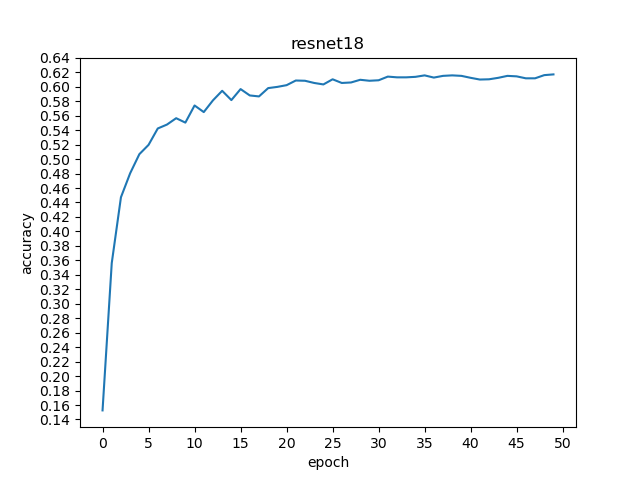
\includegraphics[width = \gw cm]{img/resnet18_epoch-accuracy.png}
	    \caption[Example of accuracy over epoch]{Example of the accuracy graphed against the number of epoch used to train for resnet18}{\centering}
	    \label{fig:res_epo_acc}
     \end{subfigure}
     \begin{subfigure}[b]{0.5\textwidth}
	    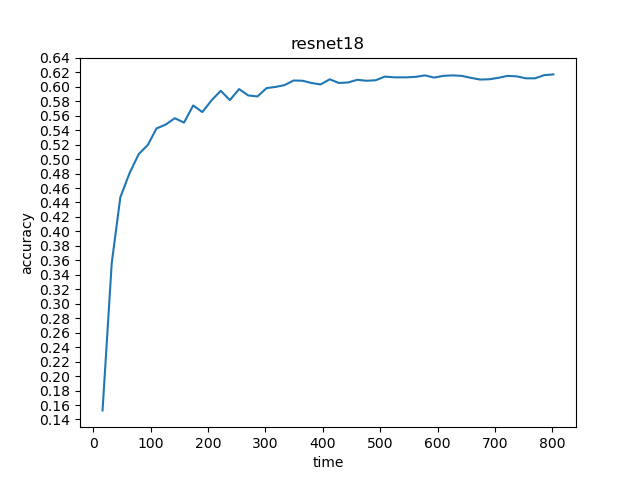
\includegraphics[width = \gw cm]{img/resnet18_time-accuracy.png}
	    \caption[Example of accuracy over time]{Example of the accuracy graphed against time taken to train in seconds for resnet18}{\centering}
	    \label{fig:res_time_acc}
     \end{subfigure}
        \caption{Example of graphs produced by the tool when analysing training time}
        \label{fig:training_time_graphs}
\end{figure}








\subsection{Analysing inference time}
As described in section n. \ref{sec:inference_time_definition} inference time is the time needed for the model to make predictions. We discussed in section n. \ref{sec:ben_inf} different ways to measure inference time, including how to calculate it considering the architecture of the Neural Network we chose. This last method, however, is not suitable for our purpose, since it is not precise enough to lead to correct predictions, therefore the method used for the benchmark tool is the one showed in Fig. n. \ref{fig:corr_inf}, with the only difference that the tool will save the prediction result and calculate the total accuracy achieved. The results will be then graphed as shown in Fig. n.\ref{fig:infere_graph}. 
\begin{figure}[h]
\centering
	    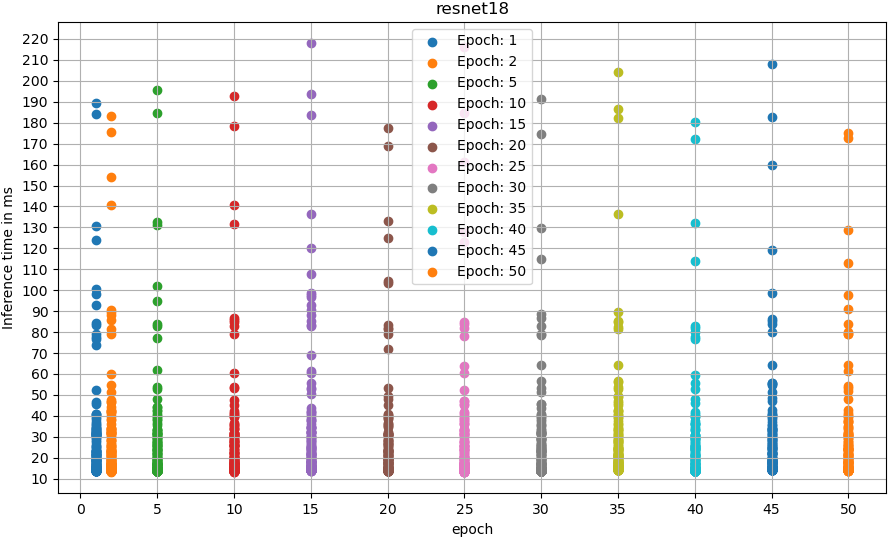
\includegraphics[width = \gw cm]{img/epoch_inferencetime.png}
        \caption{Example of the graphs produced by the tool when analysing inference time}
        \label{fig:infere_graph}
\end{figure}

Fig. n. \ref{fig:infere_graph} shows an example of Resnet18 trained for various epochs and tested using 50 images which were not part of the training set. 
During the analysis of inference time, the tool will calculate accuracy as the percentage of corrected predictions over the whole set, as shown in equation n. \ref{eq:cla_acc}. Since we are not going to treat any binary classification problem, we are going to avoid equation n. \ref{eq:bin_acc}. \\
Inference time is analysed based on the number of epochs used for training the models. A complete overview of the process is shown in Fig. n. \ref{fig:activity_diagra_inf}.\\
The user indicates a list containing all the epoch to use for training. For example, in Fig. n. \ref{fig:infere_graph} the epoch inserted were:
\[
1,2,5,10,15,20,25,30,35,40,45,50
\]
Once the model has been trained for the respective number of epoch and the inference has been tested, the results are saved and the model initialized. The process ends when the inference time of all the models have been trained for each epoch in the list. \\

\begin{figure}[th]
\centering
   \begin{tikzpicture}
       \tikzset{start/.style ={circle,minimum width=0.3cm, minimum      height=0.3cm, draw, fill}}
       
       \tikzset{activity/.style={rectangle ,minimum width=1cm,
minimum height=0.5cm, rounded corners=5pt, draw}}
        \tikzset{decision/.style={diamond,minimum width=1cm, minimum height=1cm, draw}}
        
        \tikzset{end/.style={draw,double=white, circle,
                inner sep=1pt,minimum width=0.3cm,minimum height=0.3, draw, fill}}



        \node[start] (start) {};
        %\node[activity, below of = start] (action1) {Read the configuration file};
        \node[activity, below =  of  start] (action1) {Fetch epochs list};
        \node[decision, below = of action1] (decision1) {done?};
        \node[activity, below =of  decision1] (action2) {next epoch};
        \node[activity, below =of  action2] (action3) {train models};
        \node[activity, below =of  action3] (action4) {test inference};
        \node[activity, below = of  action4] (action5) {save result};
        \node[activity, below = of  action5] (action6) {initialize models};
        
        \node[end, right =of  decision1] (end) {};

        
        \draw[->](start) -- (action1);
        \draw[->](action1) -- (decision1);
        \draw[->](decision1) -- (action2)node [left,midway]{no} ;
        \draw[->](action2) -- (action3);
        \draw[->](action3) -- (action4);
        \draw[->](action4) -- (action5);
        \draw[->](action5) -- (action6);
        \draw[->] (action6.west) -- ++(-40pt,0pt) |- (decision1.west);
        \draw[->](decision1) --  (end)node [above,midway]{yes};
   \end{tikzpicture}
   \caption{Overview of the process to test inference}
   \label{fig:activity_diagra_inf}
\end{figure}
\subsection{Further Analysis on the Metrics}
Once the tests terminate the tool stores the information collected in a file on the disk. The information stored are:
\begin{itemize}
\item Epoch
\item Training loss
\item Validation loss
\item Accuracy
\item Training time for epoch
\item Inference Time
\item Prediction
\item Ground Truth
\end{itemize}
The data, however, it is serialized before saved, therefore it can be visualized and further investigated with the use of a ready-to-use Jupyter notebook (\cite{Kluyver2016jupyter}). In addition to the raw visualization of the data, the notebook allows the user to elaborate information for further analysis. This notebook calculates the average training time needed for each epoch, the highest accuracy achieved during training and the highest accuracy during the prediction test.  Furthermore, it also calculates precision (equation n. \ref{eq:pre}), recall (equation n. \ref{eq:rec}) and the F1-score (equation n. \ref{eq:f1_score}). \\
The notebook gives also the possibility to graph the trend of the single models during the test both over training time and epochs. In addition to the trend during training as discussed in section n. \ref{sec:training_process_bench}, it is also possible to visualize the validation loss and training loss over training time. 

\chapter{Analysis of the characteristics}\label{ana_char}
\section{Introduction}
In this chapter, we will analyse and measure different characteristics from various neural network architecture with the purpose of finding useful correlations which we can use in a later stage. In order to achieve this goal, we will use our understandings from chapter \ref{char_nn} of each metric of Neural Network and the tool we developed in section \ref{sec:my_bench}. \\
In challenges such as the ImageNet classification challenge (\cite{ILSVRC15}) the ultimate goal is to achieve the highest accuracy possible, neglecting other performance metrics like inference time. \cite{DBLP:journals/corr/CanzianiPC16}\\
Although accuracy is of high importance, in practical applications other metrics are to be considered as well, depending on the different requirements. As pointed out by \textit{Canziani et al.} in \cite{DBLP:journals/corr/CanzianiPC16}, metrics like inference time, parameters and operations count are hard constraints
for the deployment of Neural Networks in practical applications. Furthermore, training time is often a time consuming process which highly depends on factors like the complexity of the task, size of the network and training set(\cite{118273}). \\
Finding relations between these metrics and other factors as well, like influence of a given input feature to the prediction of the model (\cite{hooker2019benchmark}), will allow us to optimize applications, saving time and resources in the process.

\section{Environment use for the test}
All the experiments have been run on the same machine running Ubuntu 20.04.3 LTS (Focal Fossa). For the specific of the machine, please refer to table \ref{tab:gpu_info}


\begin{table}[h]
\centering
\begin{tabular}{|l  |r|}
 \hline
CPU & AMD EPYC 7452 32-Core Processor\\
CPU MHz&                     1499.324\\
CPU max MHz&                     2350,0000\\
CPU min MHz&                     1500,0000\\
Total memory&       1056709772 kB\\
GPU&    Nvidia A100-PCIE-40GB\\
Number of GPUs & 8\\
\hline
\end{tabular}
\caption{Specifics of the machine which run the experiments}
\label{tab:gpu_info}
\end{table}






\section{Datasets and Training Methodology}\label{sec:data_models}
It is assumed for all the experiments that, if no specification is made, the training of the models has been carried out by the \textit{fit\_one\_cycle()} function present in fastai using the default learning rate. Furthermore, the models have not been pre-trained, hence no transferred learning is applied, and the models have been trained using full precision. \\
For each experiment we use rather different datasets, some of which are not related to the farming world. In the first experiment, we use the dataset proposed by \textit{Vevaldi et al.} in \cite{parkhi12a}, which will be referred to as "the Pets dataset" for the rest of the paper. This dataset is directly accessible from the library and contains 37 category of pets, with roughly 200 pictures each. \\
For the second experiment, we are going to use the dataset proposed by \textit{Giselsson et al.} in \cite{giselsson2017public}, which we are going to refer to as the ‘plant\_seedlings\_v2’ dataset. This dataset contains \textasciitilde 1000 RGB images with a resolution of 10 pixels per mm divided in 12 different plant spices. The plants in the dataset are listed in table \ref{tab:dataset_species}. This dataset contains pictures of one of the most common weed found in sugar beets plantations, a plant commonly referred to as ''charlock''. \cite{cioni_weed_2010}\\
Even though the dataset is mainly focused on seedlings and it contains pictures of other plants as well, this will give us proper insights of the models' behaviours in a farming settings. 
\begin{table}[ht]
\centering
\begin{tabular}{|c|c|c|}
\hline
    English & Latin \\
\hline
    Maize & Zea mays L.\\
    Common wheat & Tricicum aestivum L.\\
    Sugar beet & Beta vulgaris var. altissima\\
    Scentless Mayweed & Matricaria perforata Mérat\\
    Common Chickweed & Stellaria media\\
    Shepherd’s Purse & Capsella bursa-pastoris\\
    Cleavers& Galium aparine L.\\
    Redshank& Polygonum persicaria L.\\
    Charlock& Sinapis arvensis L.\\
    Fat Hen& Chenopodium album L.\\
    Small-flowered Cranesbill & Geranium pusillum\\
    Field Pansy& Viola arvensis\\
    Black-grass& Alopecurus myosuroides\\
    Loose Silky-bent& Apera spica-venti\\
    \hline
\end{tabular}
\caption[Categories of the ‘plant\_seedlings\_v2’ dataset]{Categories of the ‘plant\_seedlings\_v2’ dataset \cite{giselsson2017public} }
\label{tab:dataset_species}
\end{table}


%\hfill
\section{First experiment}


As mentioned in section \ref{sec:data_models}, this experiment has been carried out using a data-set which is rather far from the agricultural field. However, it already gives us some insights of what is to come. \\
The first metrics we are going to analyse are number of epochs, training time and accuracy. We will study those metrics to be able to recognize some patterns and use those to be able to find correlations between the three with the final aim of being able to predict one of them knowing the others. These prediction patterns can be used to save time during the learning process in future applications, as we can estimate the accuracy before starting the process.  \\
The benchmarking tool run the test for each model using three different amounts of epochs, i.e. different training time, in order to simulate three different scenarios: one example with low training time,one with a medium training time and finally one with a very high training time. The tool run with ten, fifty and 100 epochs respectively. \\
The one scenario which yield more promising results and the one we are going to analyse first is the one with fifty epochs. Fig. \ref{fig:com_ep_ac_models} shows the results of each model's accuracy graphed against the number of epochs used for training, while  Fig. \ref{fig:com_ti_ac_models} shows the results of each model's accuracy graphed against the necessary training time needed to reach that accuracy.\\




\begin{figure}[h]
       \centering 
	    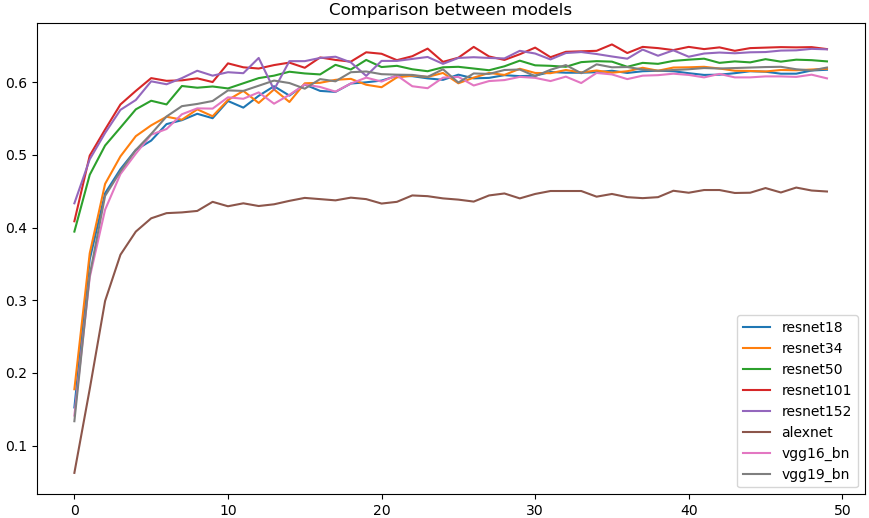
\includegraphics[width = 12 cm]{epoch-accuracy_comparison.png}
        \caption[Comparison between epoch/accuracy for each model]{Comparison between epoch/accuracy for each model. The x axis is the number of epoch, while the y axis is the accuracy achieved}
         \label{fig:com_ep_ac_models}
     \end{figure}
\begin{figure}[h]
\centering 
	    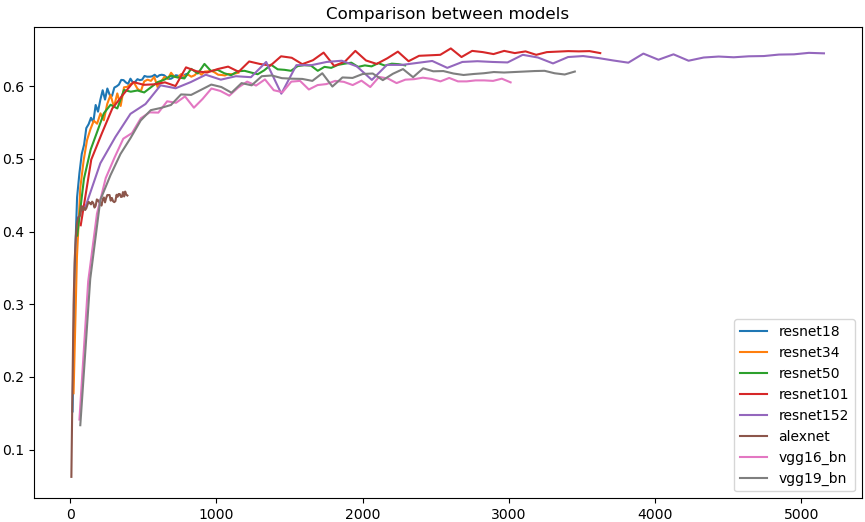
\includegraphics[width = 12 cm]{time-accuracy_comparison.png}
        \caption[Comparison between training time/accuracy for each model]{Comparison between training time/accuracy for each model. The x axis is the training time in seconds, while the y axis is the accuracy achieved}
        \label{fig:com_ti_ac_models}
\end{figure}



As suspected, for each model, the accuracy grows logarithmically higher as the number of  epochs increments, or as the training time increments. A closer inspection of Fig. \ref{fig:com_ti_ac_models} lets us derive other conclusions. Alexnet finishes training in considerably less time compared to the other networks(\textasciitilde 6 minutes), reaching however the lowest accuracy overall(45\%). We can observe this difference in time by looking at Fig.\ref{fig:sing_acc_train2} and Fig.\ref{fig:sing_acc_train}, which shows the behaviour of Alexnet, Resnet101, Resnet152 and VGG19 in the same settings. \\
As also shown in the previous graphs, Resnet101 reached overall the better accuracy at around 65\% with a training time of \textasciitilde 62 minutes, second only to Resnet152, which needed  \textasciitilde 90 minutes to reach an accuracy of \textasciitilde 64\%. Finally, VGG19 took \textasciitilde 60 minutes to reach an accuracy of 61\%. \\
In order to collect more information about the response of the model, we should take a closer look to how they performed individually.\\

\begin{figure}[h]
     \begin{subfigure}{0.5\textwidth}
	    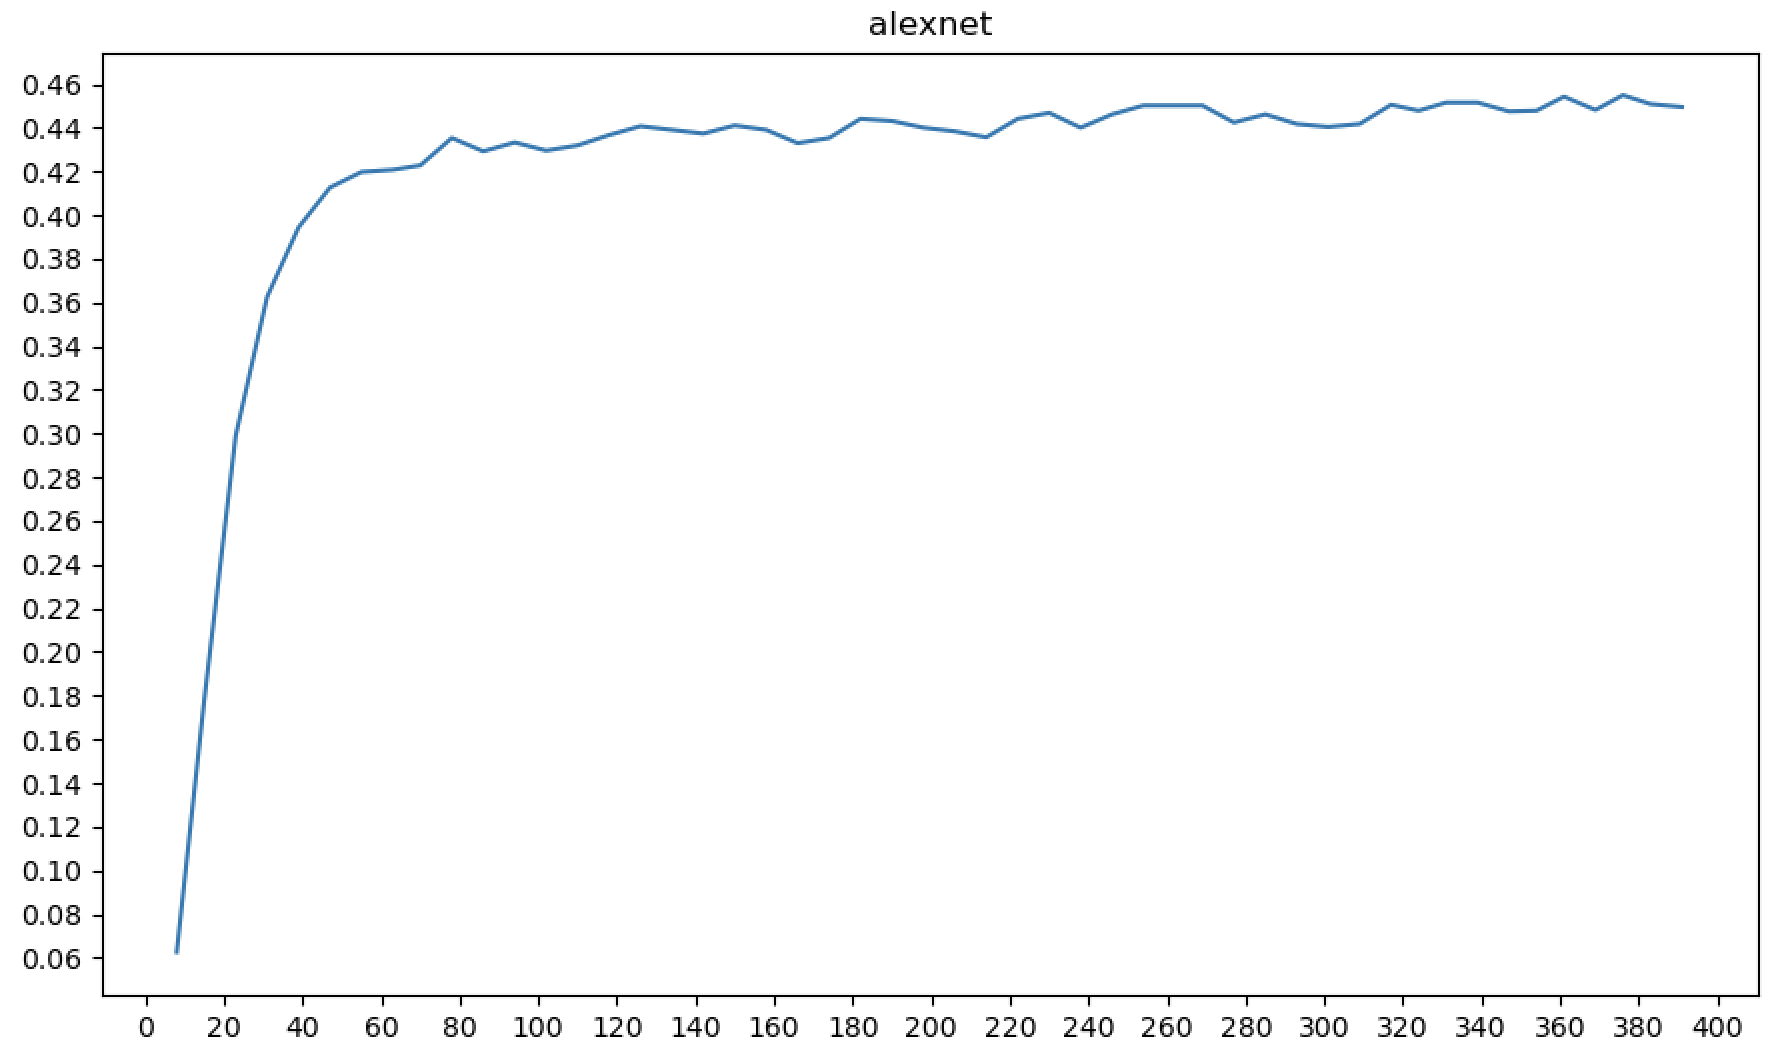
\includegraphics[width = \gws cm]{alexnet_acc_train.png}
         \label{fig:alexnet_acc_train}
     \end{subfigure}
     \hfill
     \begin{subfigure}{0.5\textwidth}
	    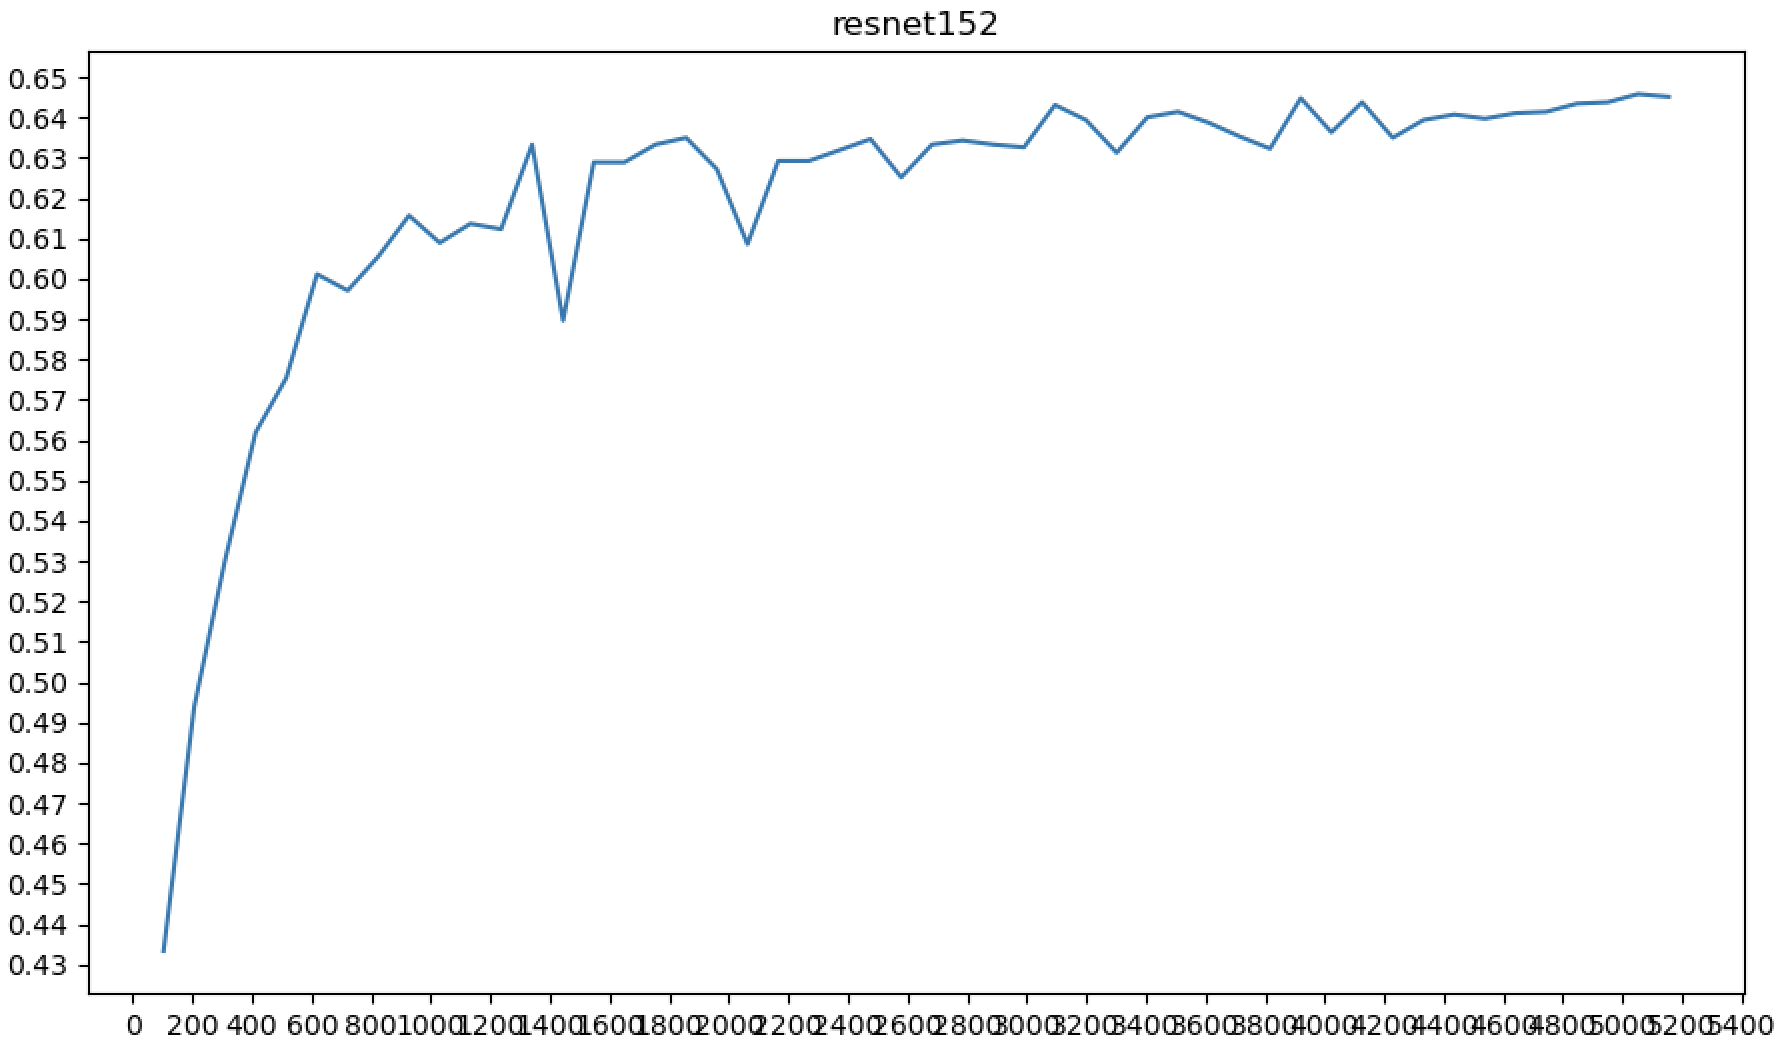
\includegraphics[width = \gws cm]{resnet_152_acc_train.png}
        \label{fig:resnet_152_acc_train}
     \end{subfigure}\\
     \caption{Accuracy of Alexnet and Resnet152 against training time in seconds}
        \label{fig:sing_acc_train2}
\end{figure}
\begin{figure}[h]
     \begin{subfigure}{0.5\textwidth}
	    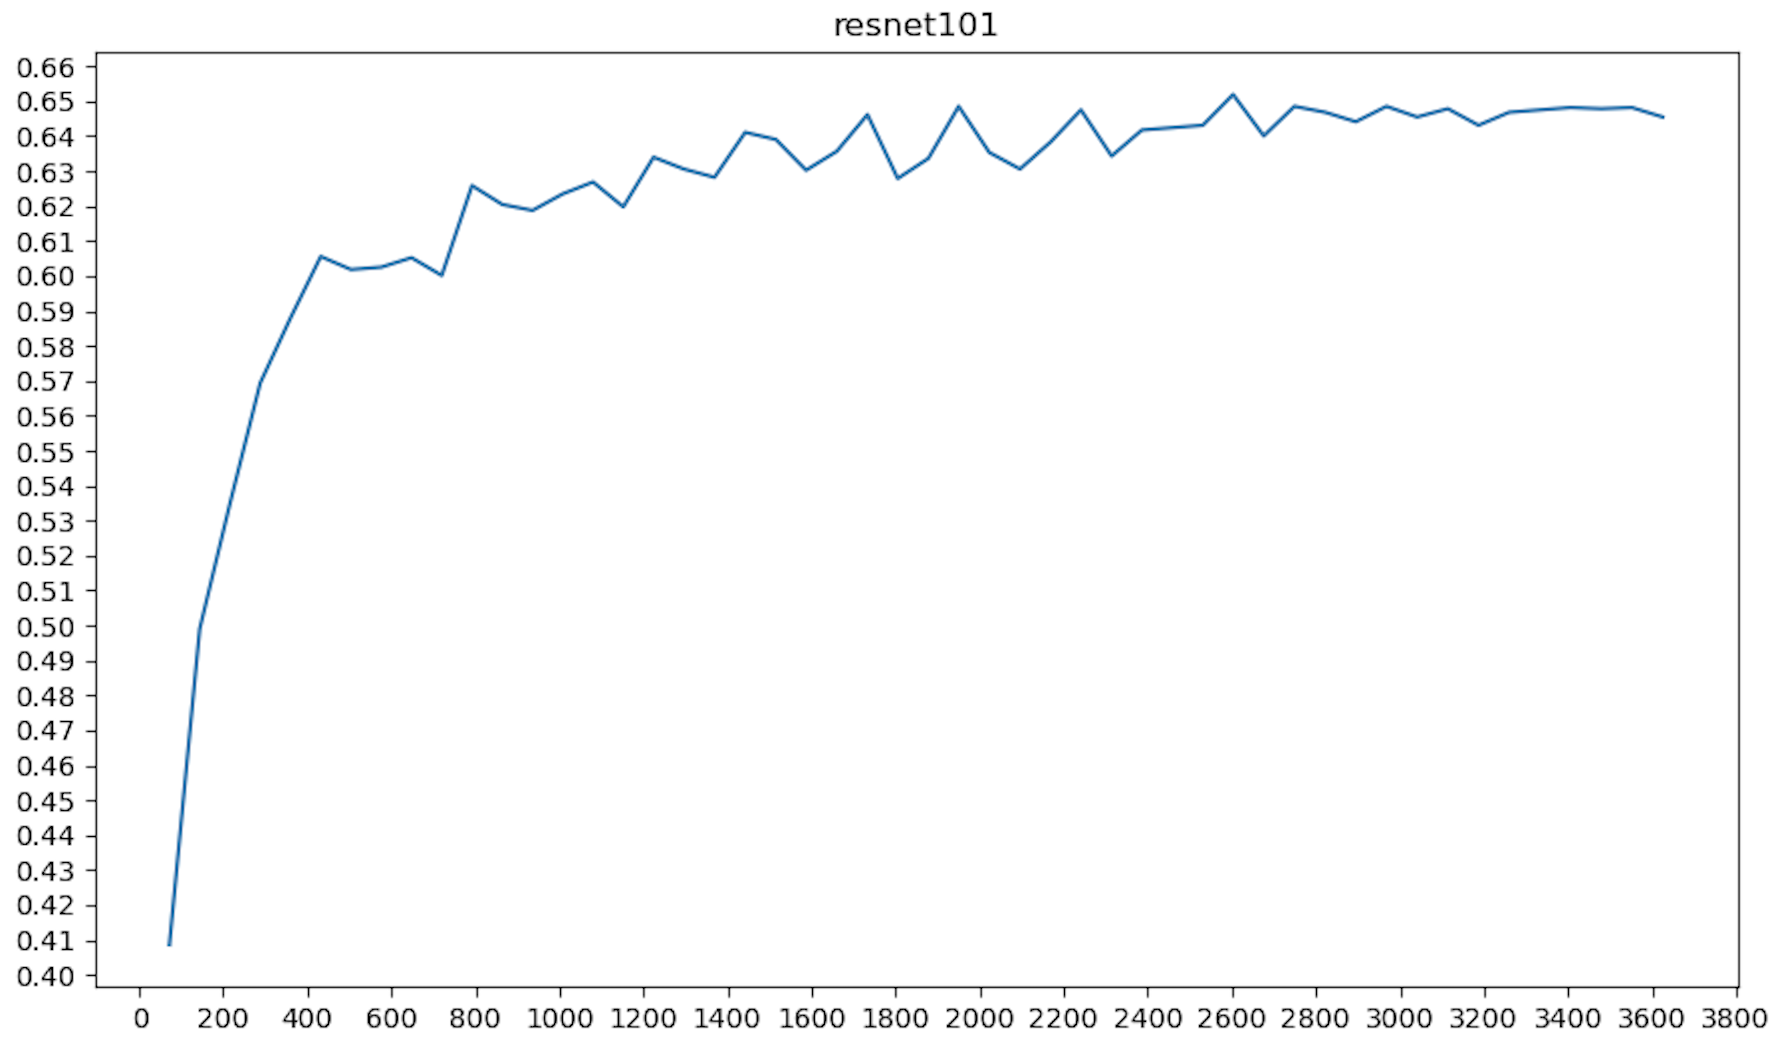
\includegraphics[width = \gws cm]{resnet_101_acc_train.png}
        \label{fig:resnet_1o1_acc_train}
     \end{subfigure}
     \begin{subfigure}{0.5\textwidth}
	    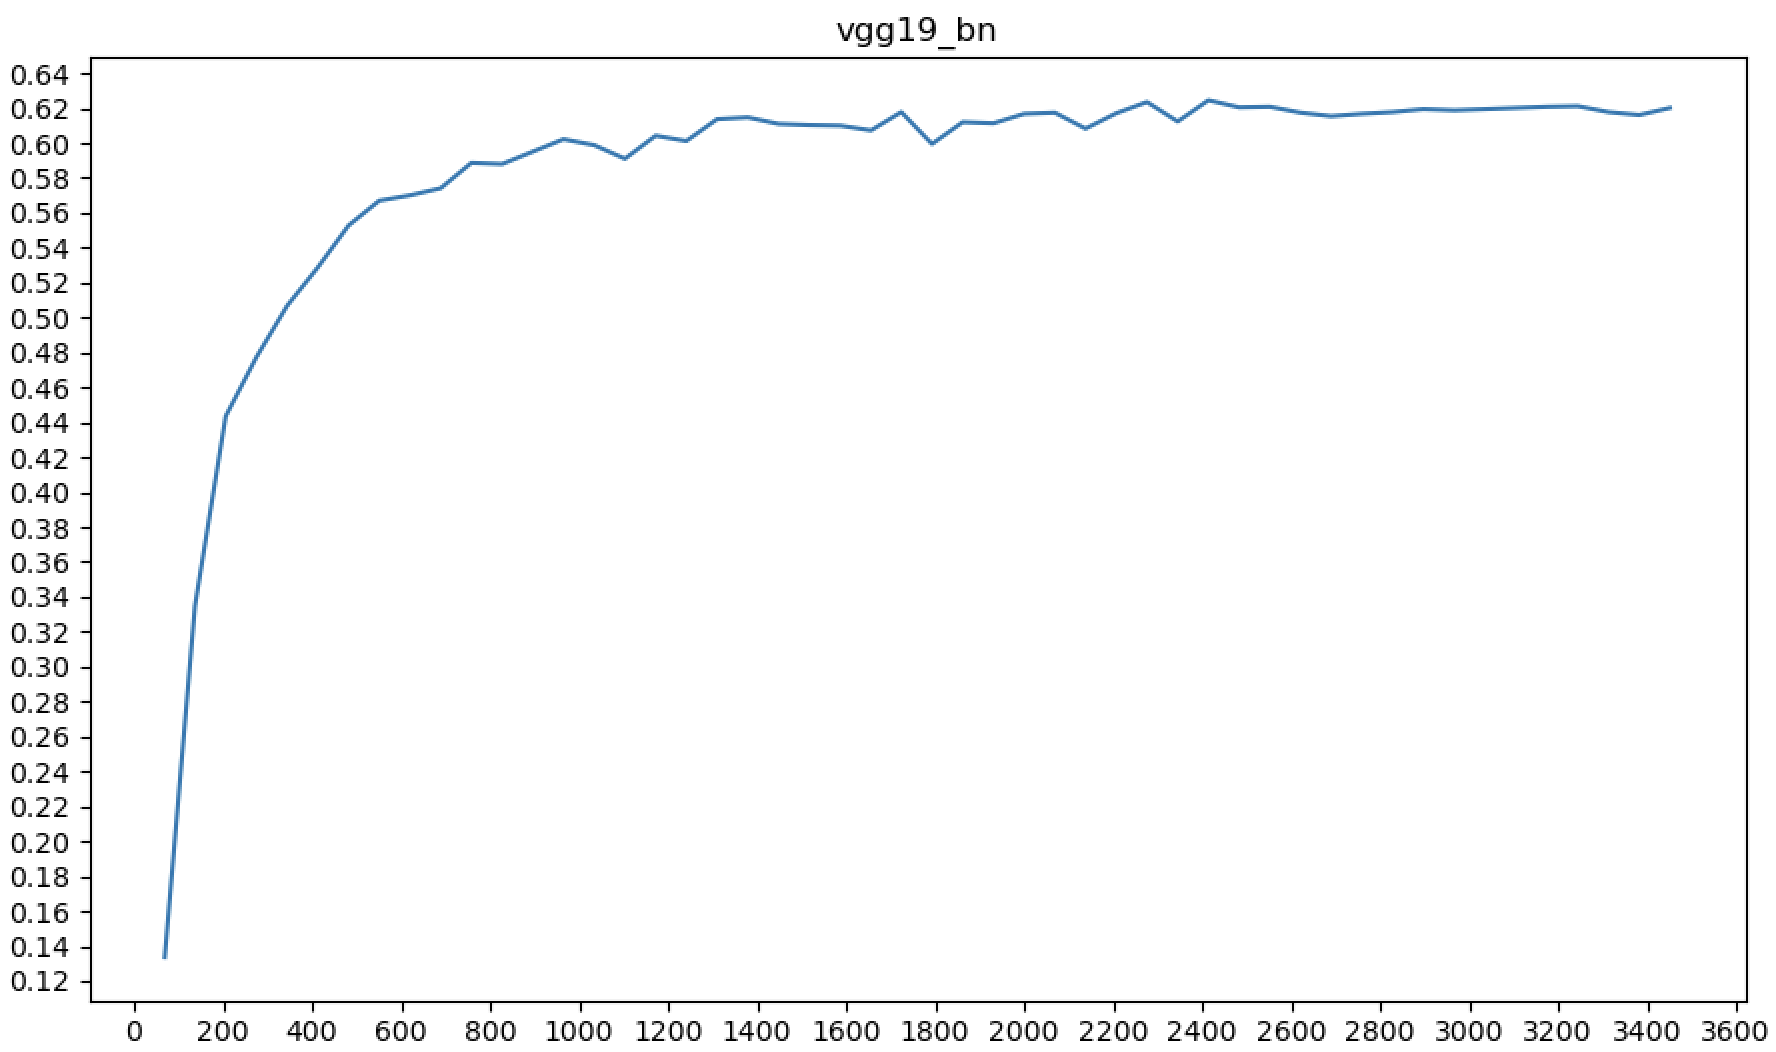
\includegraphics[width = \gws cm]{vgg_19_acc_train.png}
        \label{fig:vgg_19_acc_train}
     \end{subfigure}
        \caption{Accuracy of Resnet101 and VGG9 against training time in seconds}
        \label{fig:sing_acc_train}
\end{figure}
Fig.\ref{fig:sing_acc_train2} and Fig.\ref{fig:sing_acc_train} also show how stable each model were during training. The stability we are observing right now is how fluctuating each model has been during training regarding its accuracy. The less fluctuating it is, the better we able to predict the accuracy from training time or number of epoch, and vice-versa. From the results, we can see that Resnet152 and Resnet101 tend to fluctuate more compared to Alexnet or VGG19 (Fig. \ref{fig:sing_acc_train}). \\
Such fluctuation, however, does not hide a trend which is in common amongst all models: after a certain number of epochs, the accuracy tends to stabilize and grow significantly slower. Fig. \ref{fig:com_ep_ac_models} can help us locate the point at which the accuracy stops increasing at a high rate at around 10 epochs and this is further proved by Fig. \ref{fig:sing_acc_ep}.\\
\begin{figure}[h]
     \begin{subfigure}{0.5\textwidth}
	    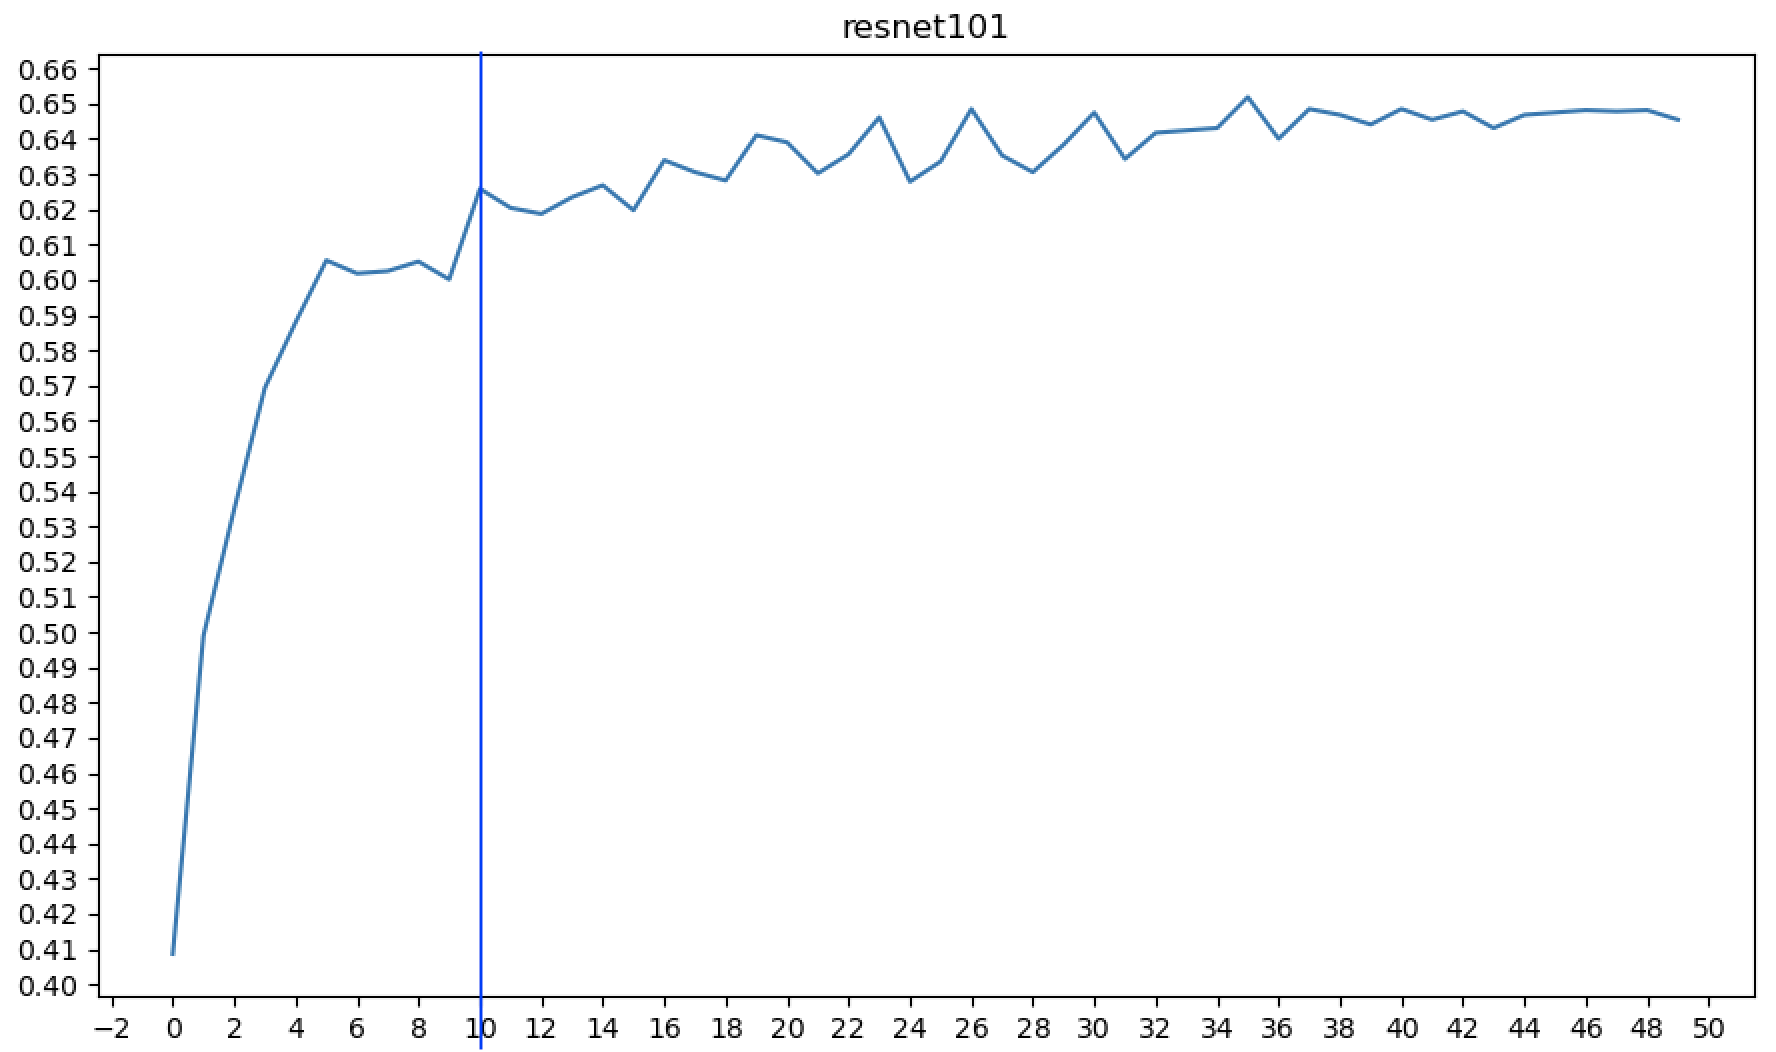
\includegraphics[width = \gws cm]{resnet_101_acc_ep.png}
        \label{fig:resnet_101_acc_ep}
     \end{subfigure}
     \begin{subfigure}{0.5\textwidth}
	    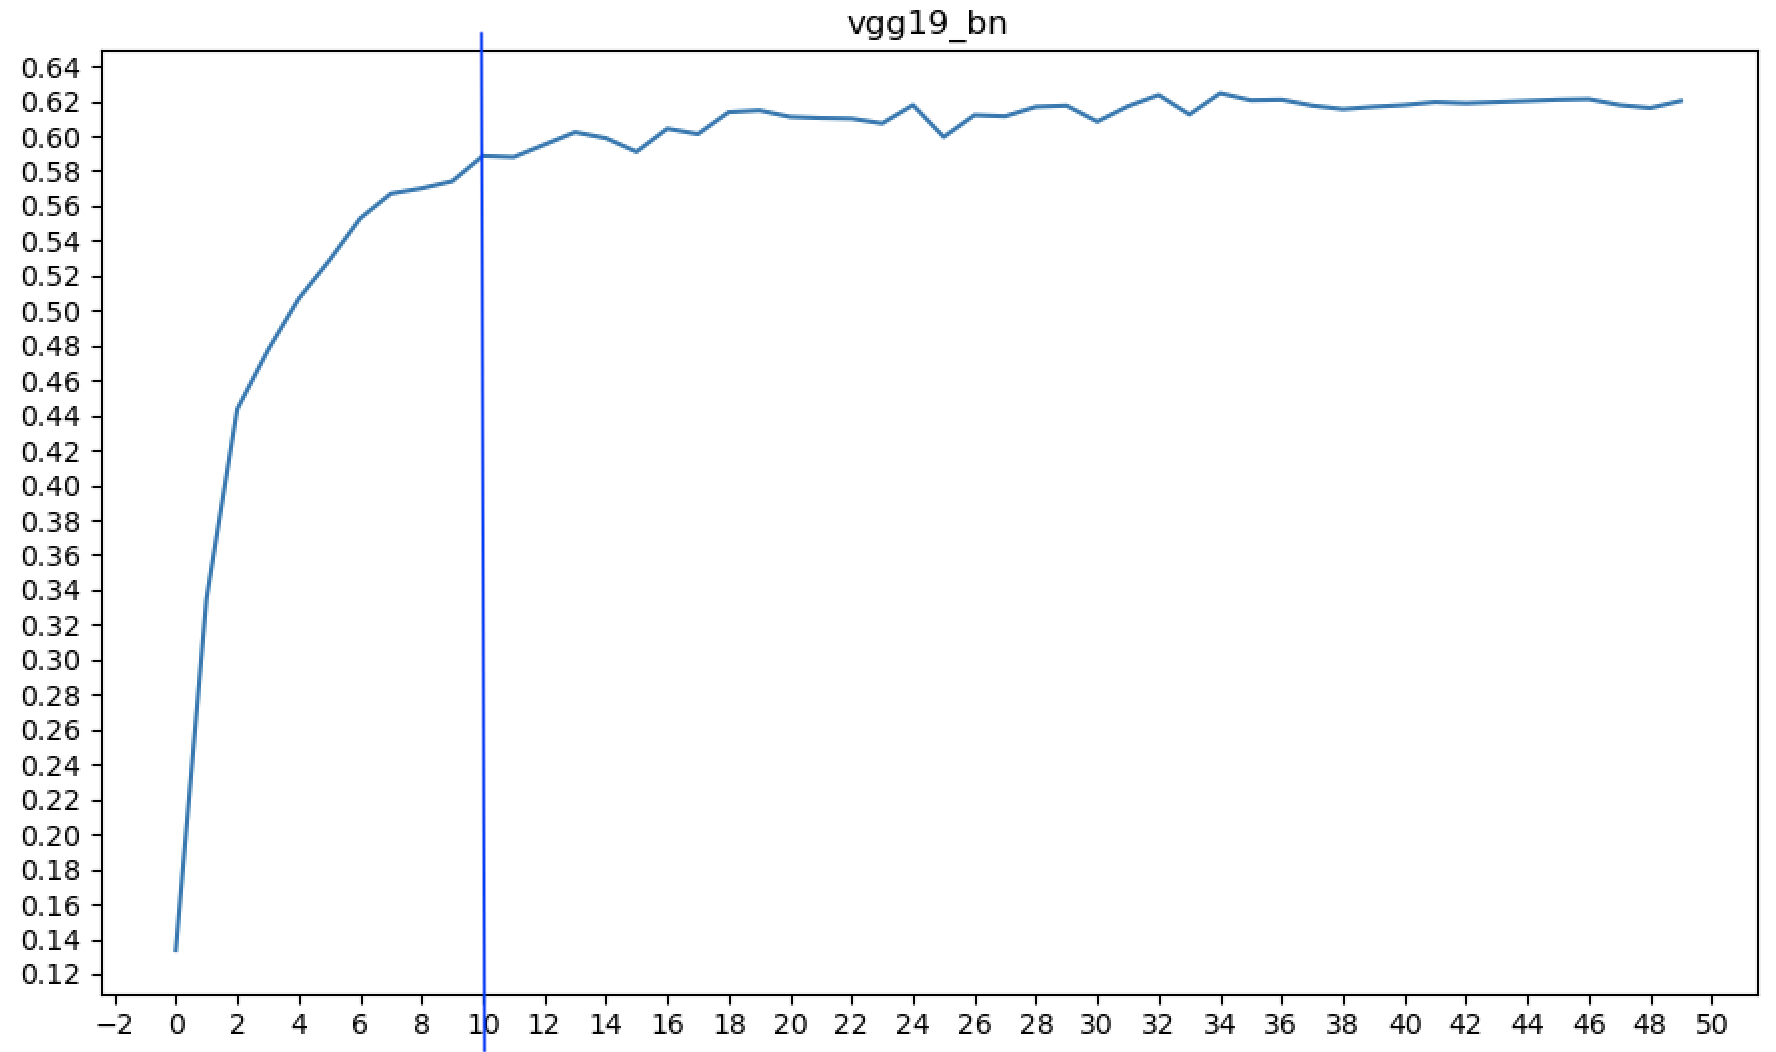
\includegraphics[width = \gws cm]{vgg_19_acc_ep.png}
        \label{fig:vgg_19_acc_ep}
     \end{subfigure}
        \caption{Breaking point of Resnet101 and VGG19}
        \label{fig:sing_acc_ep}
\end{figure}\\



We can further analyse the behaviour of each models for the first 10 epochs by observing Fig. \ref{fig:acc_training_10}. This graph gives us a closer look to how the models have been trained and how the curve looks like. Differently from the previous graph, Resnet152 this time reached a higher accuracy, however it was also the models who took the most time to fully complete the training.\\
On the other hand, from Fig. \ref{fig:acc_training_10}, we can clearly observe  that, if compared with each other for the same training time, shallower networks like Resnet34 or Resnet50 achieved higher accuracy than deeper networks like Resnet152. This is obviously due to the fact that within the same training time shallower networks manage to complete more epochs, therefore complete more training cycles. As a matter of fact, if we were to compare models on an epoch base we will find that deeper networks will achieve better accuracy given the same number of epochs. \\
If we observe Fig. \ref{fig:com_ti_ac_models} before the 1000 seconds mark, we can see that Resnet18's curve starts to flatten reaching an accuracy of \textasciitilde 61\%, while the others tend to reach smaller accuracy values. Around the 1000 seconds marks the behaviour of all the models starts to equalize and afterwards the accuracy of deeper networks will increase reaching higher values. As mentioned previously, this is due to the models being able to finish more epochs within the same time frame. In this case, the models reached to finish the training completely, as shown in \ref{fig:com_ti_ac_models}. 
Models from different architectures do not follow this trend. Alexnet, as we already discussed above, does not manage to reach somewhat close to the same accuracy of the other models. VGG16 and VGG19 follow similar trends and both curves overlap multiple times.  Even though VGG19 is considerably bigger than VGG16 (\cite{simonyan2015deep}), they reach very similar accuracy even before the 1000 seconds marks with very similar training time. \\
\begin{figure}[h]
       \centering 
	    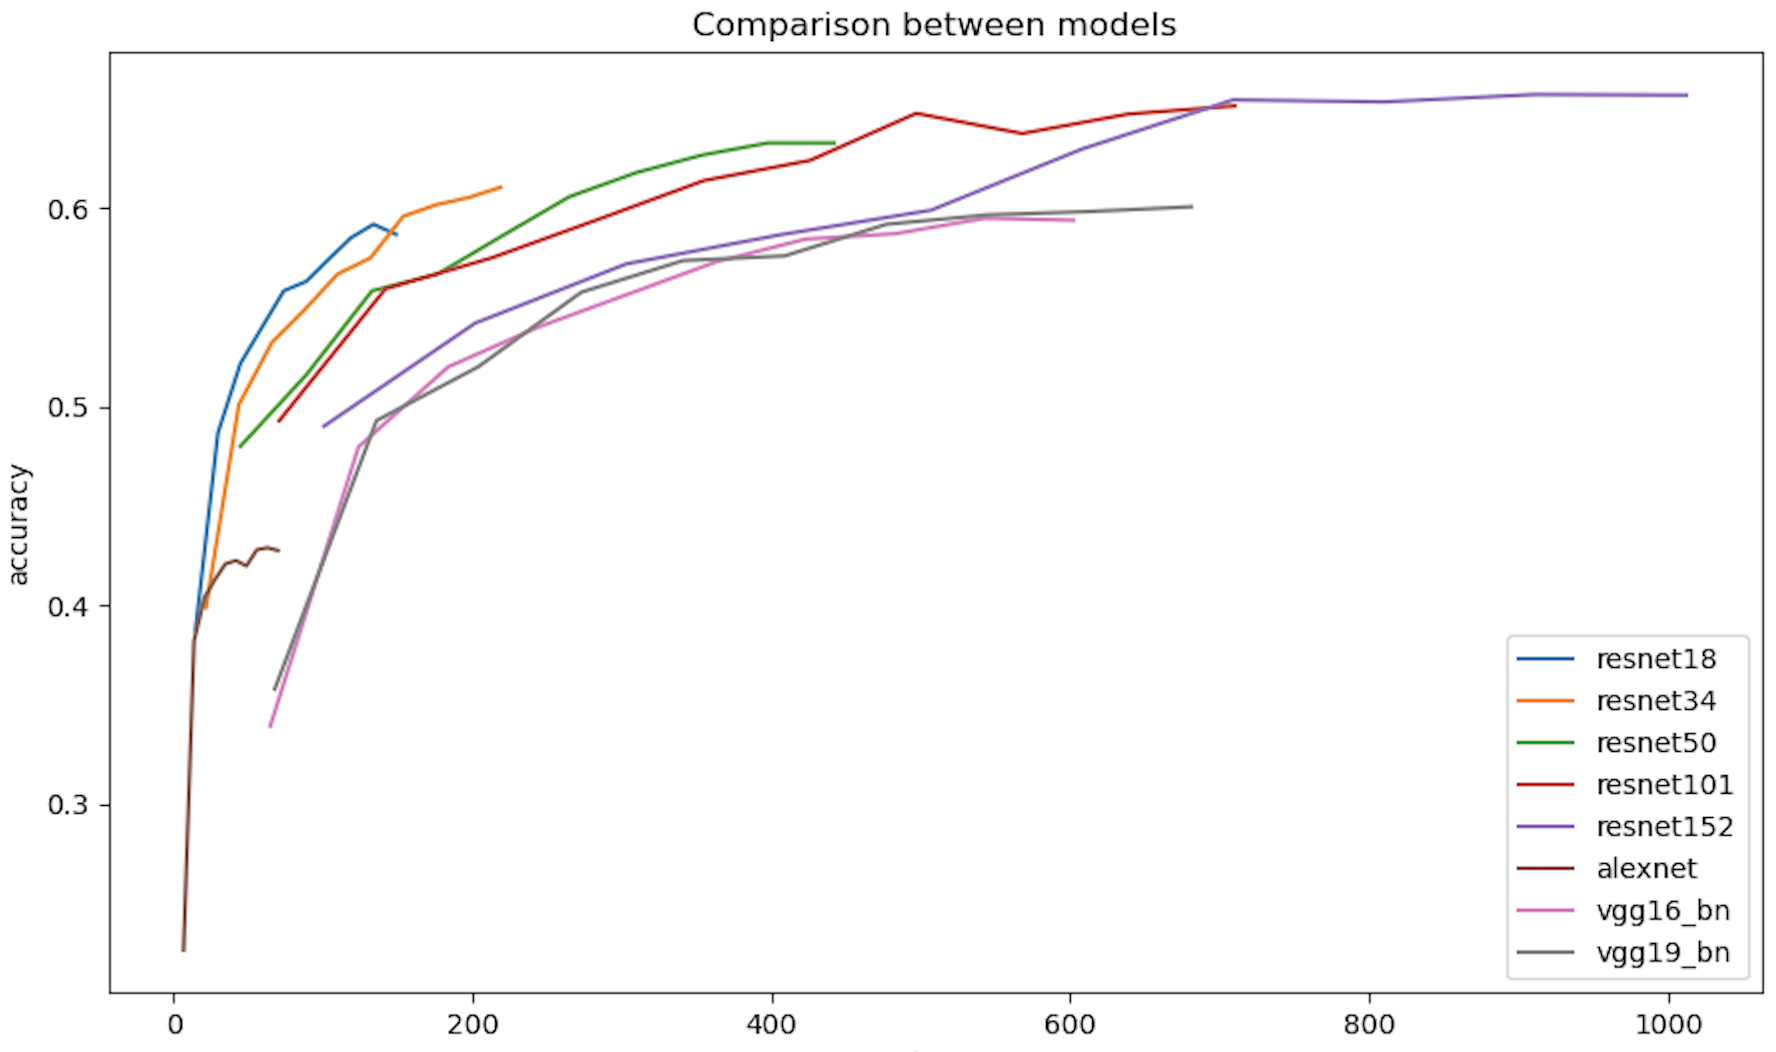
\includegraphics[width = 12 cm]{acc_training_time_10.png}
        \caption[Comparison between training time and accuracy for each model for 10 epochs]{Comparison between training time and accuracy for each model for 10 epochs. The x axis is the training time in seconds, while the y axis is the accuracy achieved}
         \label{fig:acc_training_10}
\end{figure}


\begin{figure}[h]
       \centering 
	    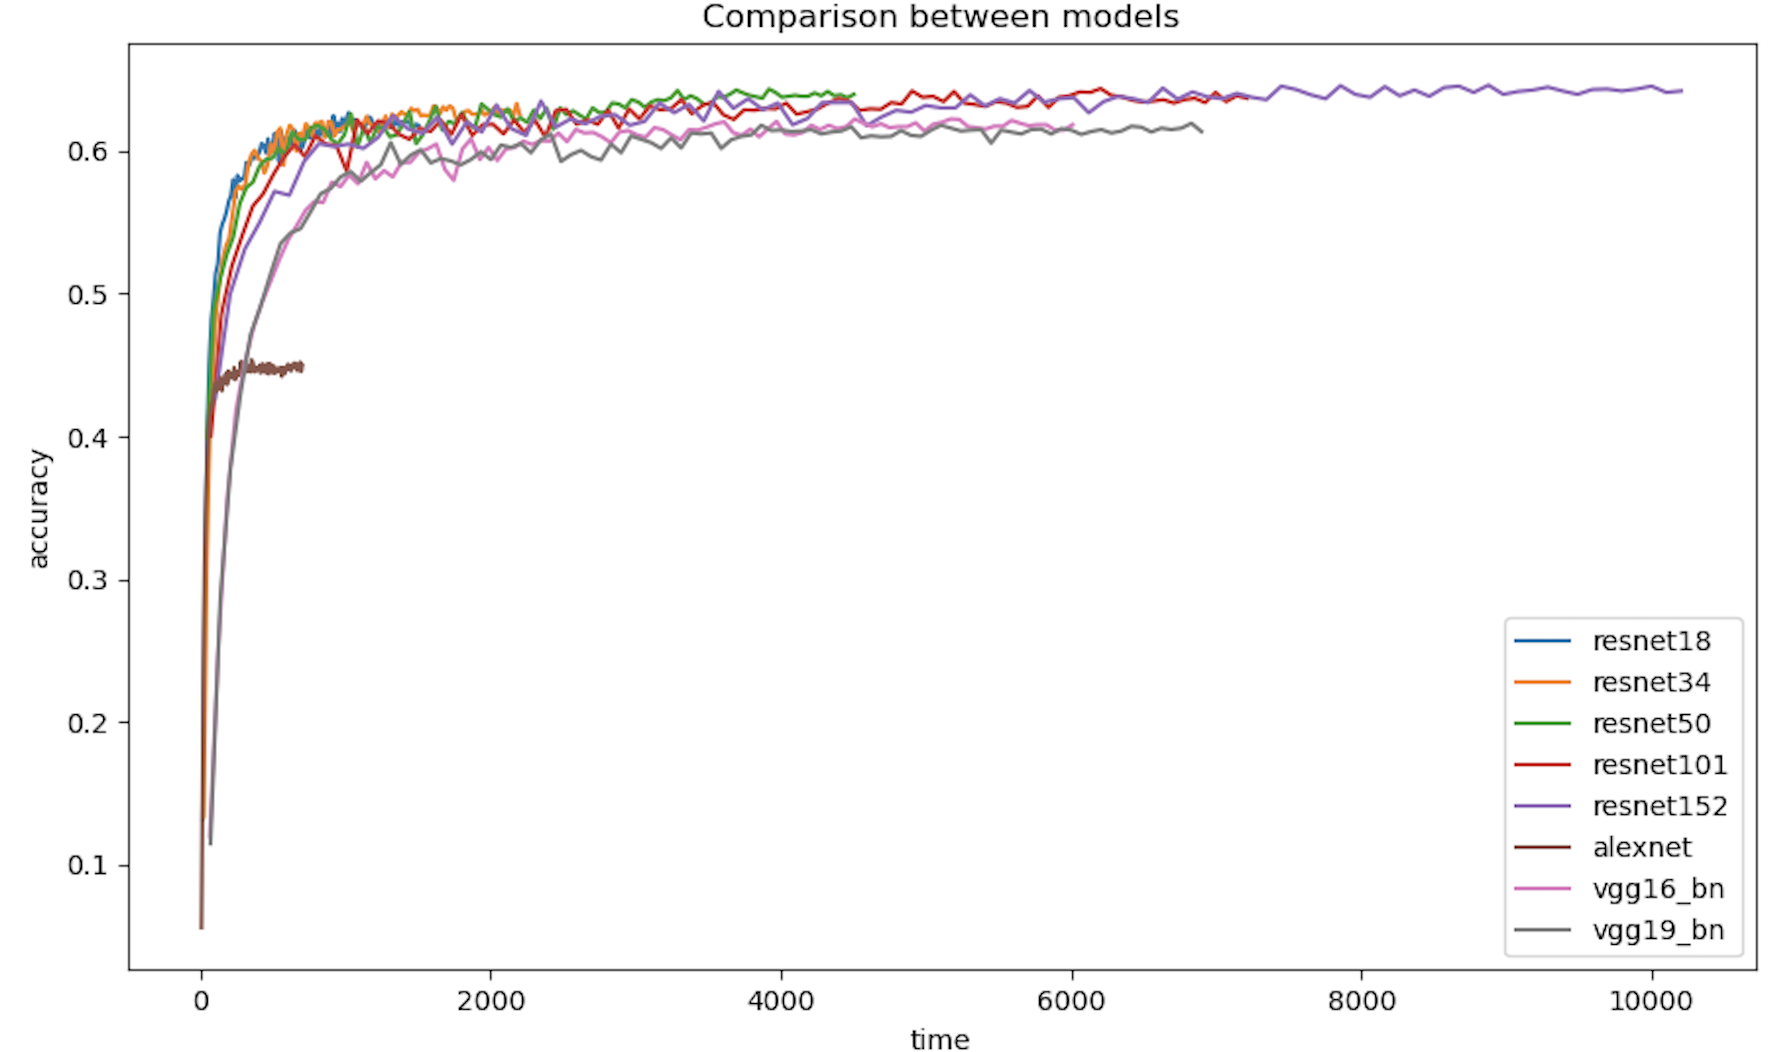
\includegraphics[width = 12 cm]{time_acc_100.png}
        \caption[Comparison between training time and accuracy for each model for 100 epochs]{Comparison between training time and accuracy for each model trained for 100 epochs. The x axis is the training time in seconds, while the y axis is the accuracy achieved}
         \label{fig:time_acc_100}
\end{figure}




This behaviour is further highlighted in Fig. \ref{fig:time_acc_100} which shows the behaviour of the models trained for 100 epochs. We can see that once again around 1000 seconds the curve of every model starts to flatten and the models using the Resnet architectures achieve similar accuracy. The highest accuracy is achieved by Resnet152, which also needed the most training time. Surprisingly, Resnet50 performed better than Resnet101 achieving better accuracy with less training time.
VGG16 and VGG19 performed similarly displaying overlapping curves, with VGG19 once again requiring more training time. \\
More importantly, however,this graph confirms the results and the hypothesis we made previously.Furthermore, we can use all the data we acquired to calculate the average training time required for each epoch. The results are provided in table \ref{tab:time_f_epoch}.
\begin{table}[h]
\centering
\begin{tabular}{ p{2cm} p{2cm}   }
 Model&Time (s)\\
 \hline
Resnet18&15.01\\
Resnet34&22.0\\
Resnet50&45.02\\
Resnet101&72.11\\
Resnet152&102.02\\
Alexnet&7.01\\
VGG16&60.09\\
VGG19&68.97\\
 \hline
\end{tabular}
\caption{Average time for each epoch}
\label{tab:time_f_epoch}
\end{table}

Training for 100 epochs gives us also more complete insights regarding the future performance of our models. In other words, we can determine when the model starts to over-fit or under-fit and when to stop the training to avoid future poor performances. \\
\begin{figure}[h]
\begin{subfigure}{0.5\textwidth}
	    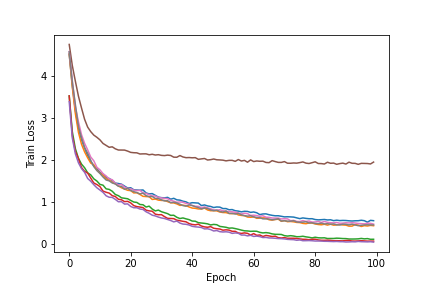
\includegraphics[width = \gws cm]{epoch_train_loss.png}
	    \caption{Training Loss calculated over 100 epochs}
        \label{fig:train_loss}
        
     \end{subfigure} \hfill
     \begin{subfigure}{0.5\textwidth}
	    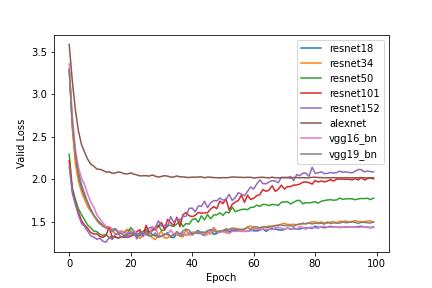
\includegraphics[width = \gws cm]{epoch_valid_loss.png}
	    \caption{Validity Loss calculated over 100 epochs}
         \label{fig:valid_loss}
         
     \end{subfigure}
    
     
     \caption{ Training loss and validity loss of all models calculated over 100 epochs}
        \label{fig:tran_valid_loss}
\end{figure}


As shown in Fig. \ref{fig:train_loss}, the train loss decreases at each epoch for each model. For Alexnet, the curve tends to flatten at around 15 epochs, while for the others it flattens at around 60. Rather than observing the training loss trend alone, however,which does not give us the possibility to comprehend correctly the response of the models, we should compare it to the trend of the validation loss shown in Fig. \ref{fig:valid_loss}. Alexnet remained stable for the duration of the training, with a validation loss comparable to the training loss. The other models, on the other hand, show a rather different behaviour. At around 20 epochs, the validation loss of deeper networks, i.e. Resnet152, Resnet101 and VGG19 starts to increment drastically. For shallower networks of the Resnet architecture, i.e. Resnet18, Resnet34 and Resnet50, and for VGG16 the validation loss decreased for the first 15 epochs and started to increment only after \textasciitilde40.\\
In section n. \ref{sec:of_uf} we defined over-fitting to be a situation in which the validation loss is much larger than training and from Fig. \ref{fig:valid_loss} we can see that, although after various number of epochs, most of the networks start to enter this condition as the validation loss increases and it becomes much larger than their training loss.We also discussed some techniques to avoid this, like for i.g. Cross-Validation. For the purpose of this experiment, we only split the dataset 80-20, hence we used no cross-validation or augmentation on the data-set whatsoever. \\
 
In addition to the training time, we can also use the benchmark tool we developed to measure and analyse the inference time of each model.\\
As we are mostly focused on sugar beet recognition, it is safe to assume use cases where field robots would scan the field to recognize the vegetation, similarly to the one proposed by \textit{Lottes et al.} in \cite{7487720}. In such setting, the time taken to classify the image results in a soft deadline, as the time taken to scan the field is greatly influenced by it, therefore being able to estimate the needed inference time could help optimize this part of the application. \\
To measure inference time, we need to collect a dataset of related pictures which are not part of the training dataset to feed to each model. For our tests, we are going to use a dataset comprising of 200 random pictures. The pictures we are going to use are going be of different dimensions and different quality in order to see if we can recognize patterns. We can see the results in Fig. \ref{fig:inf_time_epoch_c}, which displays the training time in milliseconds graphed against the accuracy and the number of epoch used to train. From this figure, we can clearly see that the inference time for every model rarely is measured to be more than 230 milliseconds, with the exception of few outliers, and most of the models for most epochs have an accuracy between 87\% and 92\%. In addition, if we analyse the inference time based on the number of epoch (Fig. \ref{fig:inf_time_epoch}) the models display similar responses.  \\


\begin{figure}[h]
     \begin{subfigure}{0.5\textwidth}
	    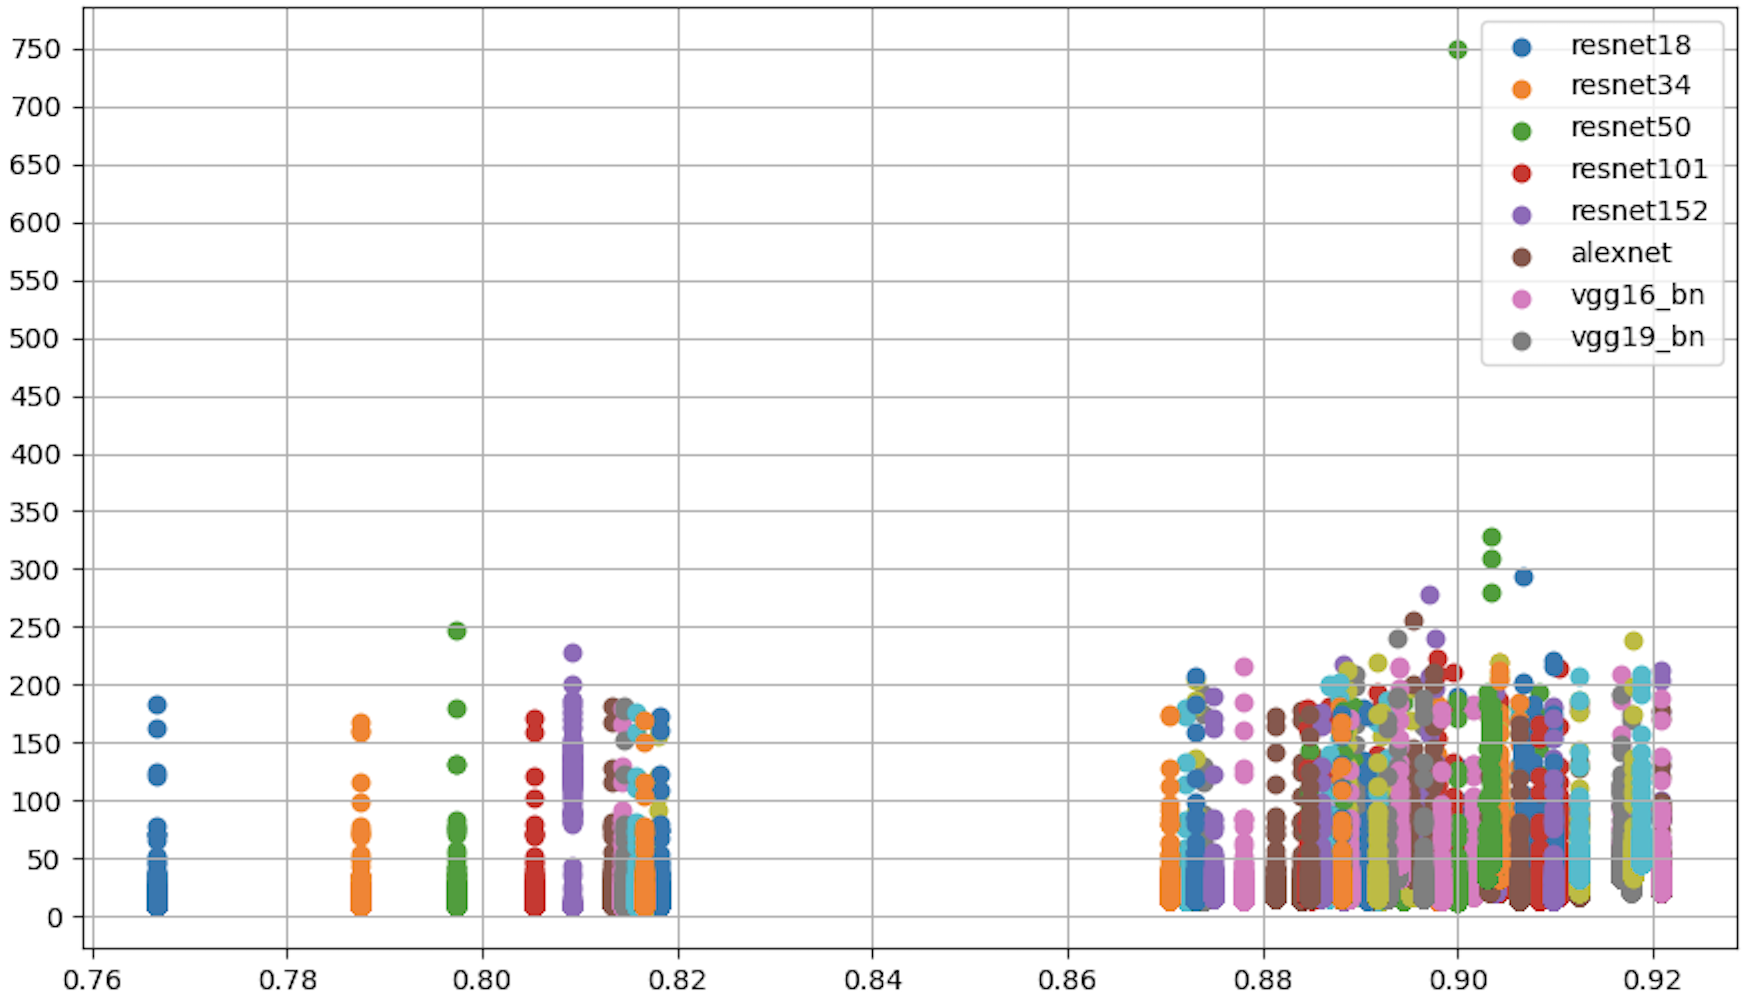
\includegraphics[width = \gws cm]{inf_time_accuracy.png}
	    \caption{}
         \label{fig:inf_time_accuracy}
     \end{subfigure}
     \hfill
     \begin{subfigure}{0.5\textwidth}
	    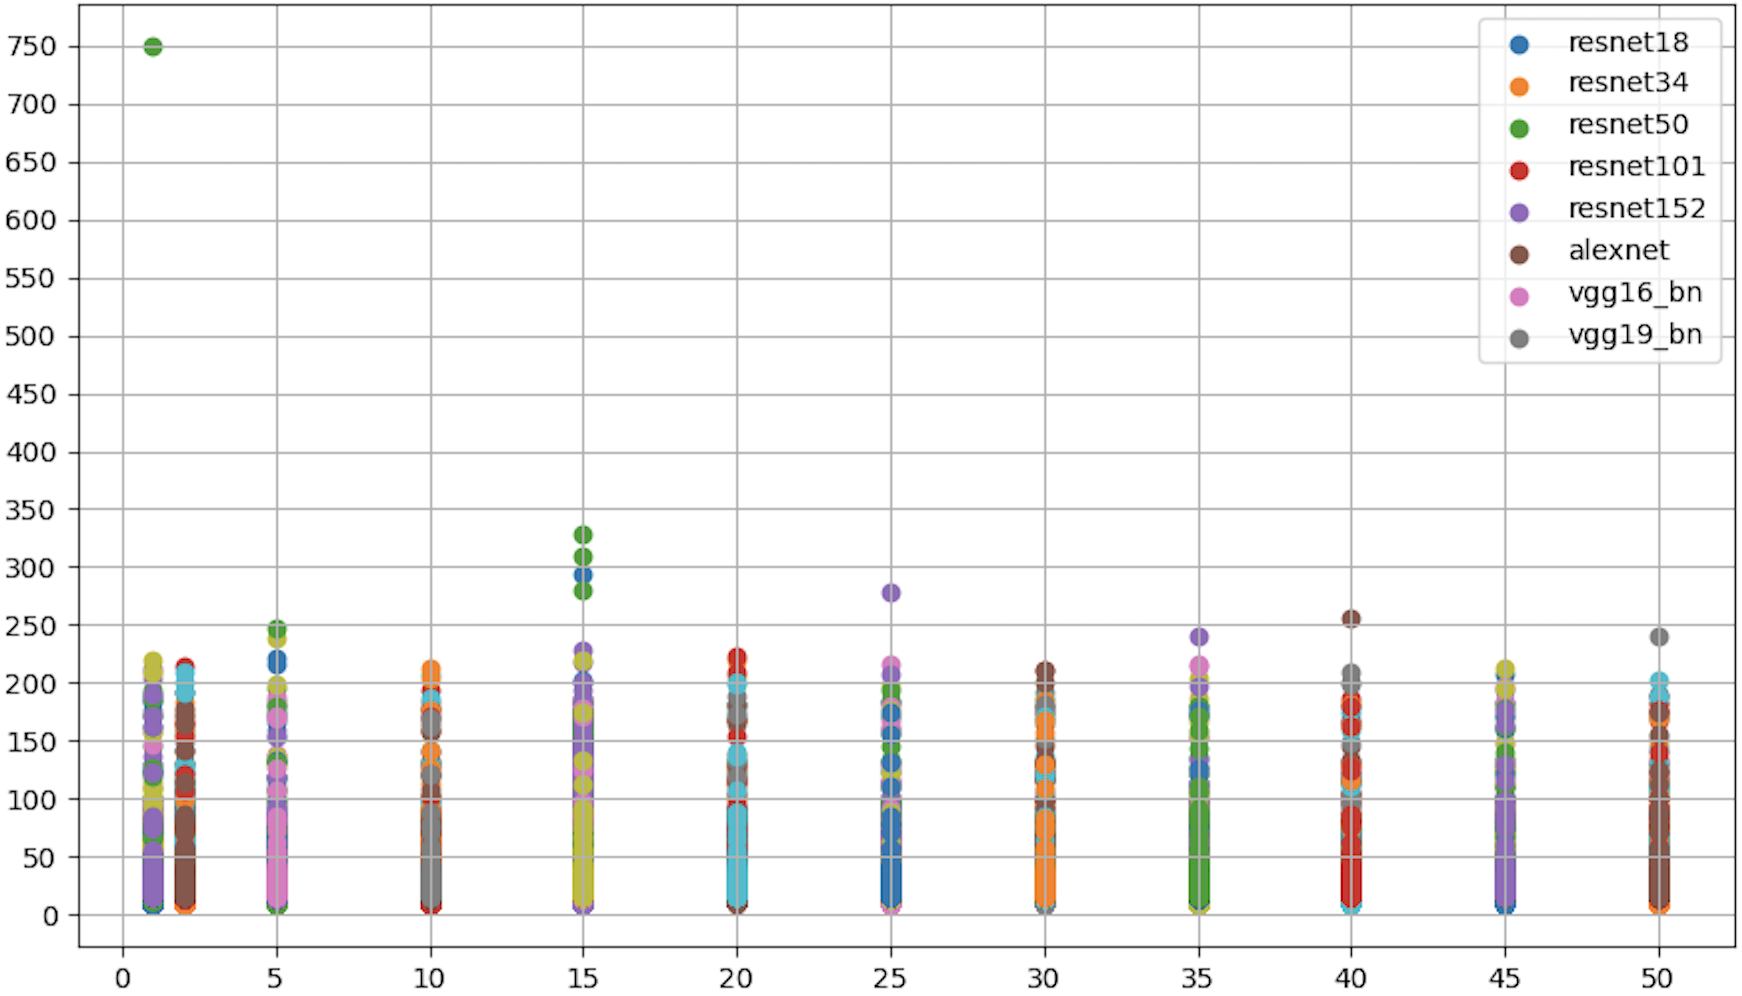
\includegraphics[width = \gws cm]{inf_time_epoch.png}
	    \caption{}
        \label{fig:inf_time_epoch}
     \end{subfigure}\\
     \caption[Inference time measured for each model]{Inference time measured for each model using the 200 pictures dataset discussed previously. The inference time is in milliseconds, while the accuracy for Fig. \ref{fig:inf_time_accuracy}is the percentage of correct predictions.}
        \label{fig:inf_time_epoch_c}
\end{figure}

\begin{figure}[h]
     \begin{subfigure}{0.5\textwidth}
	    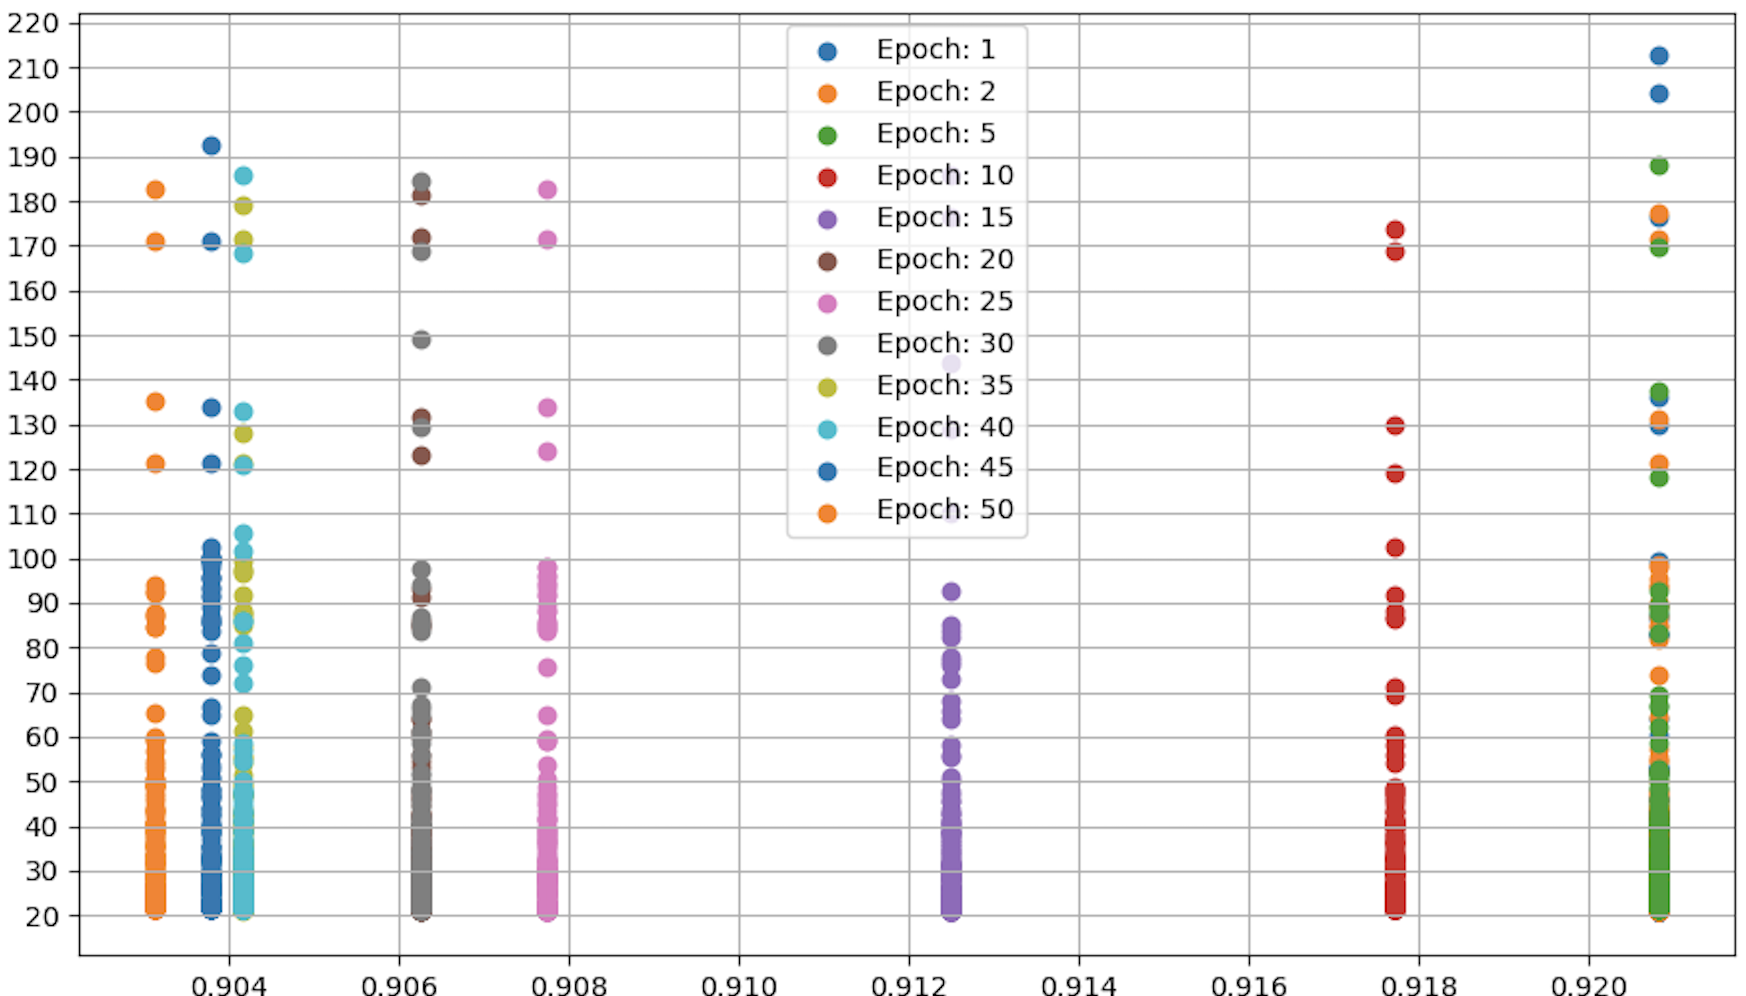
\includegraphics[width = \gws cm]{inf_acc_resnet18.png}
	    \caption{Resnet18}
         \label{fig:inf_acc_resnet18}
         
     \end{subfigure}
     \hfill
     \begin{subfigure}{0.5\textwidth}
	    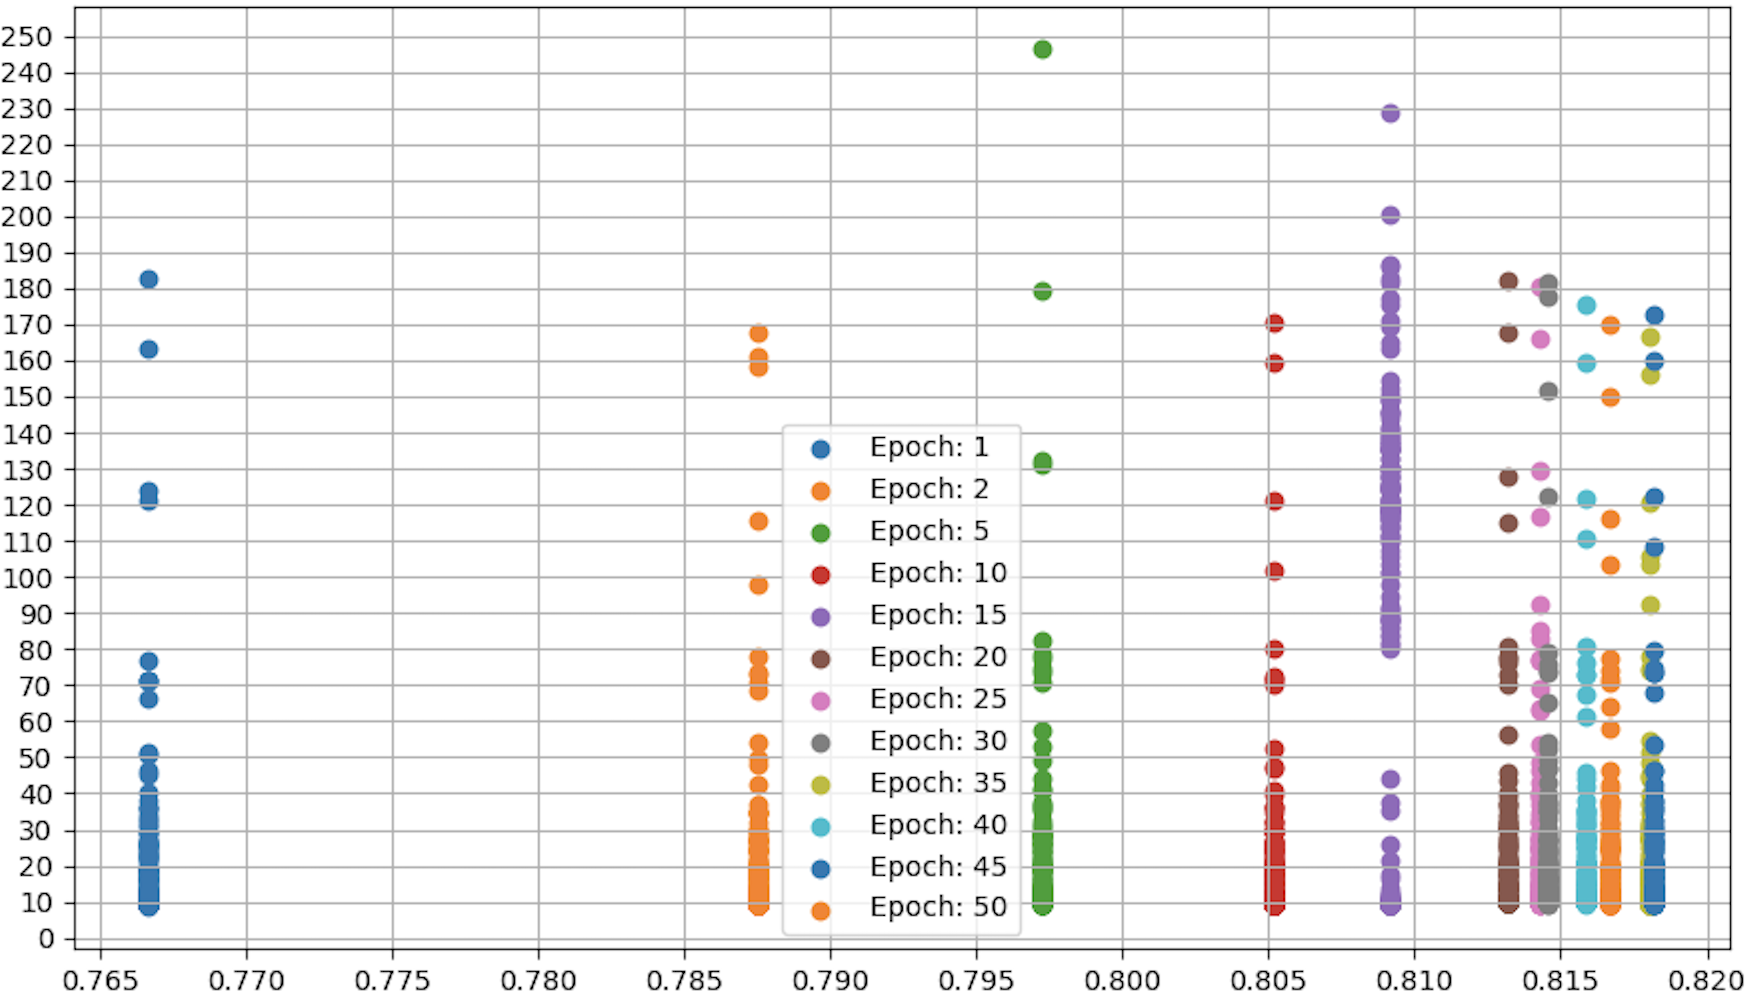
\includegraphics[width = \gws cm]{inf_acc_alexnet.png}
	    \caption{Alexnet}
        \label{fig:inf_acc_alexnet}
        
     \end{subfigure}\\
     \caption{Inference time measured for model Resnet18 and Alexnet}
        \label{fig:inf_acc_c}
\end{figure}
When we compare model individually like in Fig. \ref{fig:inf_acc_c}, other similarities appear. As a matter of fact, when we analyse each model, we can observe that some pictures require considerably more time than others. For example, Fig. \ref{fig:inf_acc_c} shows the measurements obtained by model Resnet18 (\ref{fig:inf_acc_resnet18}) and Alexnet (\ref{fig:inf_acc_alexnet}) and from their response it appears that, at each epoch, there is a constant number of images which takes more time to be processed. \\
We can run the tool once again to identify the 10 images that took more time to be processed at each epoch in order to analyse them and find elements which can explain such difference. \\
The first property of the image we are going to take a look is the size of the images. Fig. \ref{fig:size_inference_time_compared} shows the results obtained for each model. 


\begin{figure}[h]
       \centering 
	    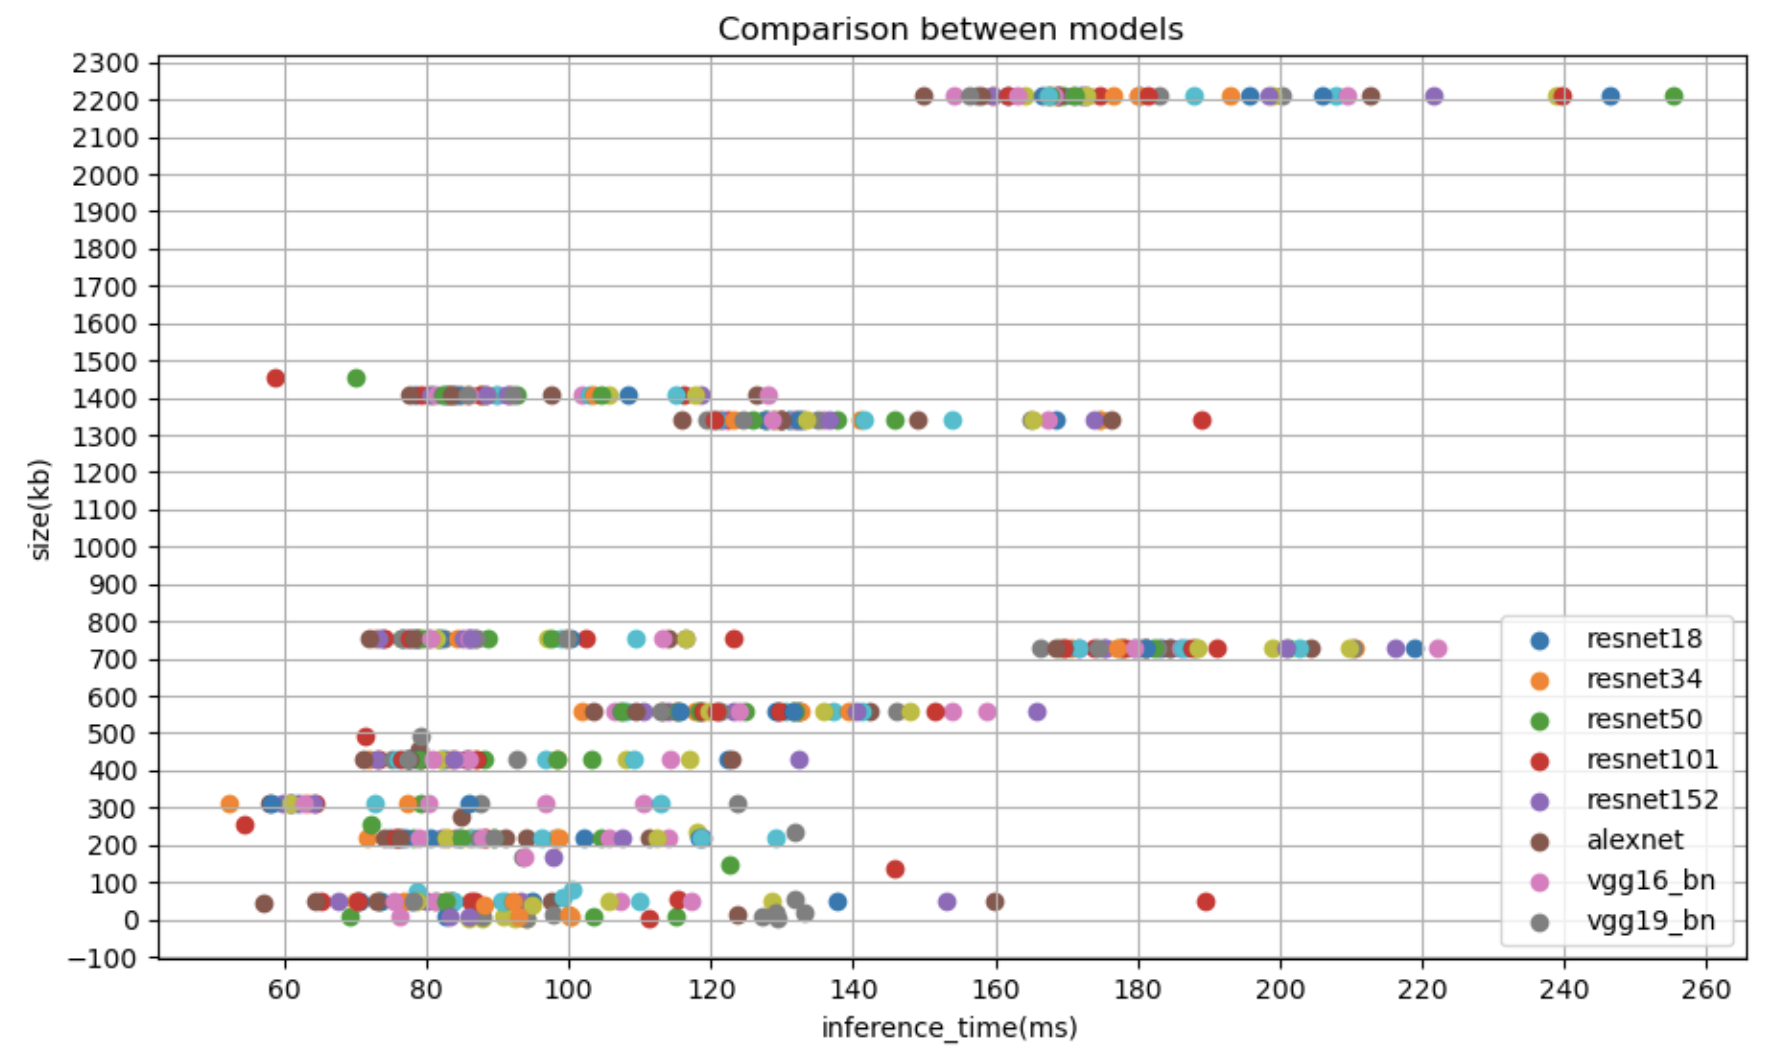
\includegraphics[width = 14 cm]{size_inference_time_compared.png}
        \caption[Size of the images over inference time]{This graph shows the size in kb of the ten slowest images over the time taken to be processed }
         \label{fig:size_inference_time_compared}
\end{figure}



From the graph we are able to spot some rather interesting behaviours. First of all, we would expect that for each epoch the slowest images would be the same. This hypothesis would be confirmed if the graph showed group of pictures of the same size having different inference time. However, this is only the case for sizes bigger than 500 kbs. As a matter of fact, we are not able to cluster pictures before 500 kbs under a certain inference time range as effectively as we can do for heavier pictures. We can conclude from this that regardless of the amount of training, pictures over 500kbs are going to be the slowest ones. \\
From a closer investigation of the individual models emerged some differences in the response of the single models. \\
For deeper networks the situation is similar to the discussion we made. As shown in Fig. \ref{fig:sl_f_deep}, for both Resnet152 and VGG16, the response for pictures smaller than 500 kb is noisy, although Resnet152 show a more stable behaviour than VGG16. This implies that for these networks only the response with images over 500kbs displays similarities.  
\begin{figure}[h]
     \begin{subfigure}{0.5\textwidth}
	    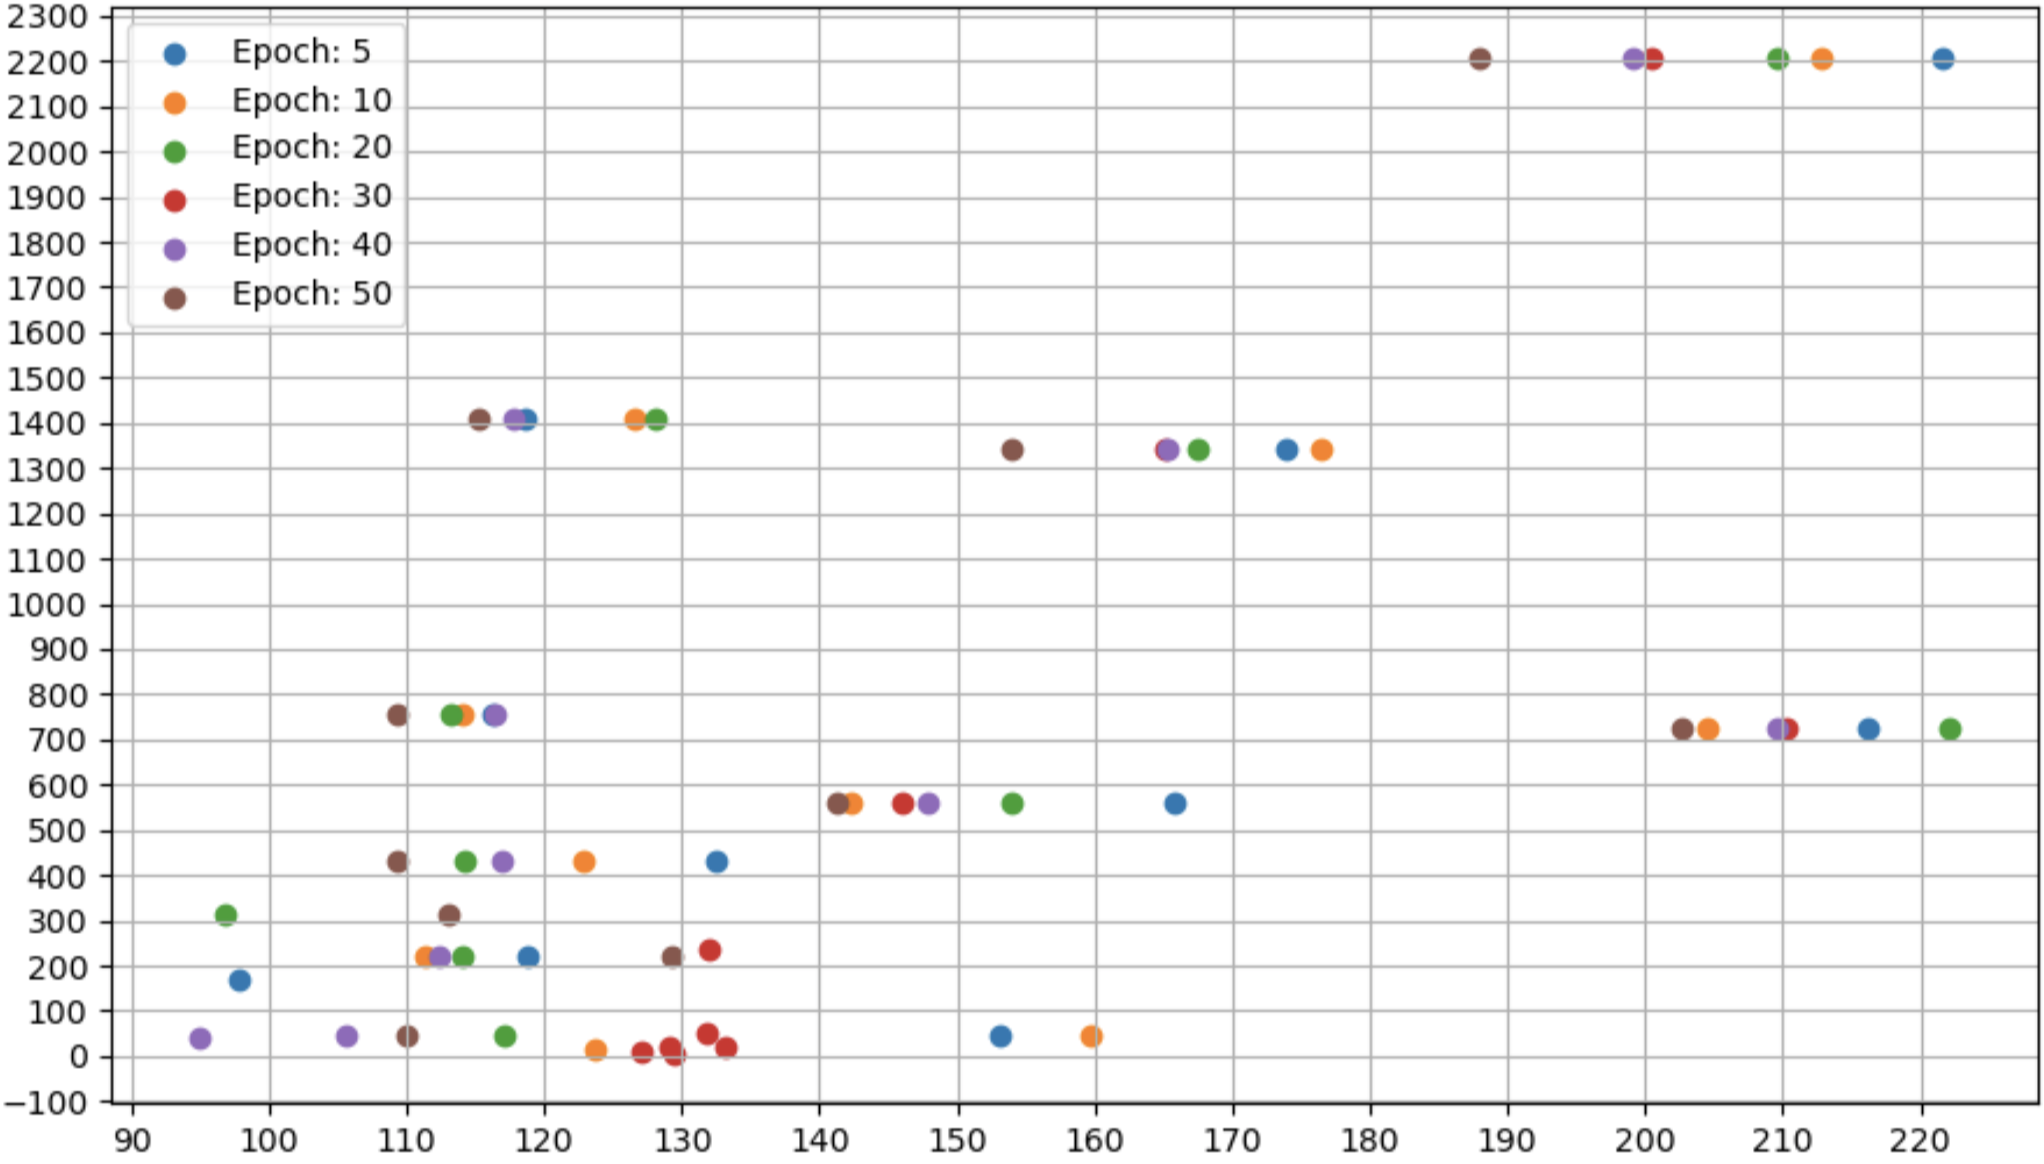
\includegraphics[width = \gws cm]{resnet152_sl_f.png}
	    \caption{Resnet152}
         \label{fig:resnet152_sl_f}
         
     \end{subfigure}
     \hfill
     \begin{subfigure}{0.5\textwidth}
	    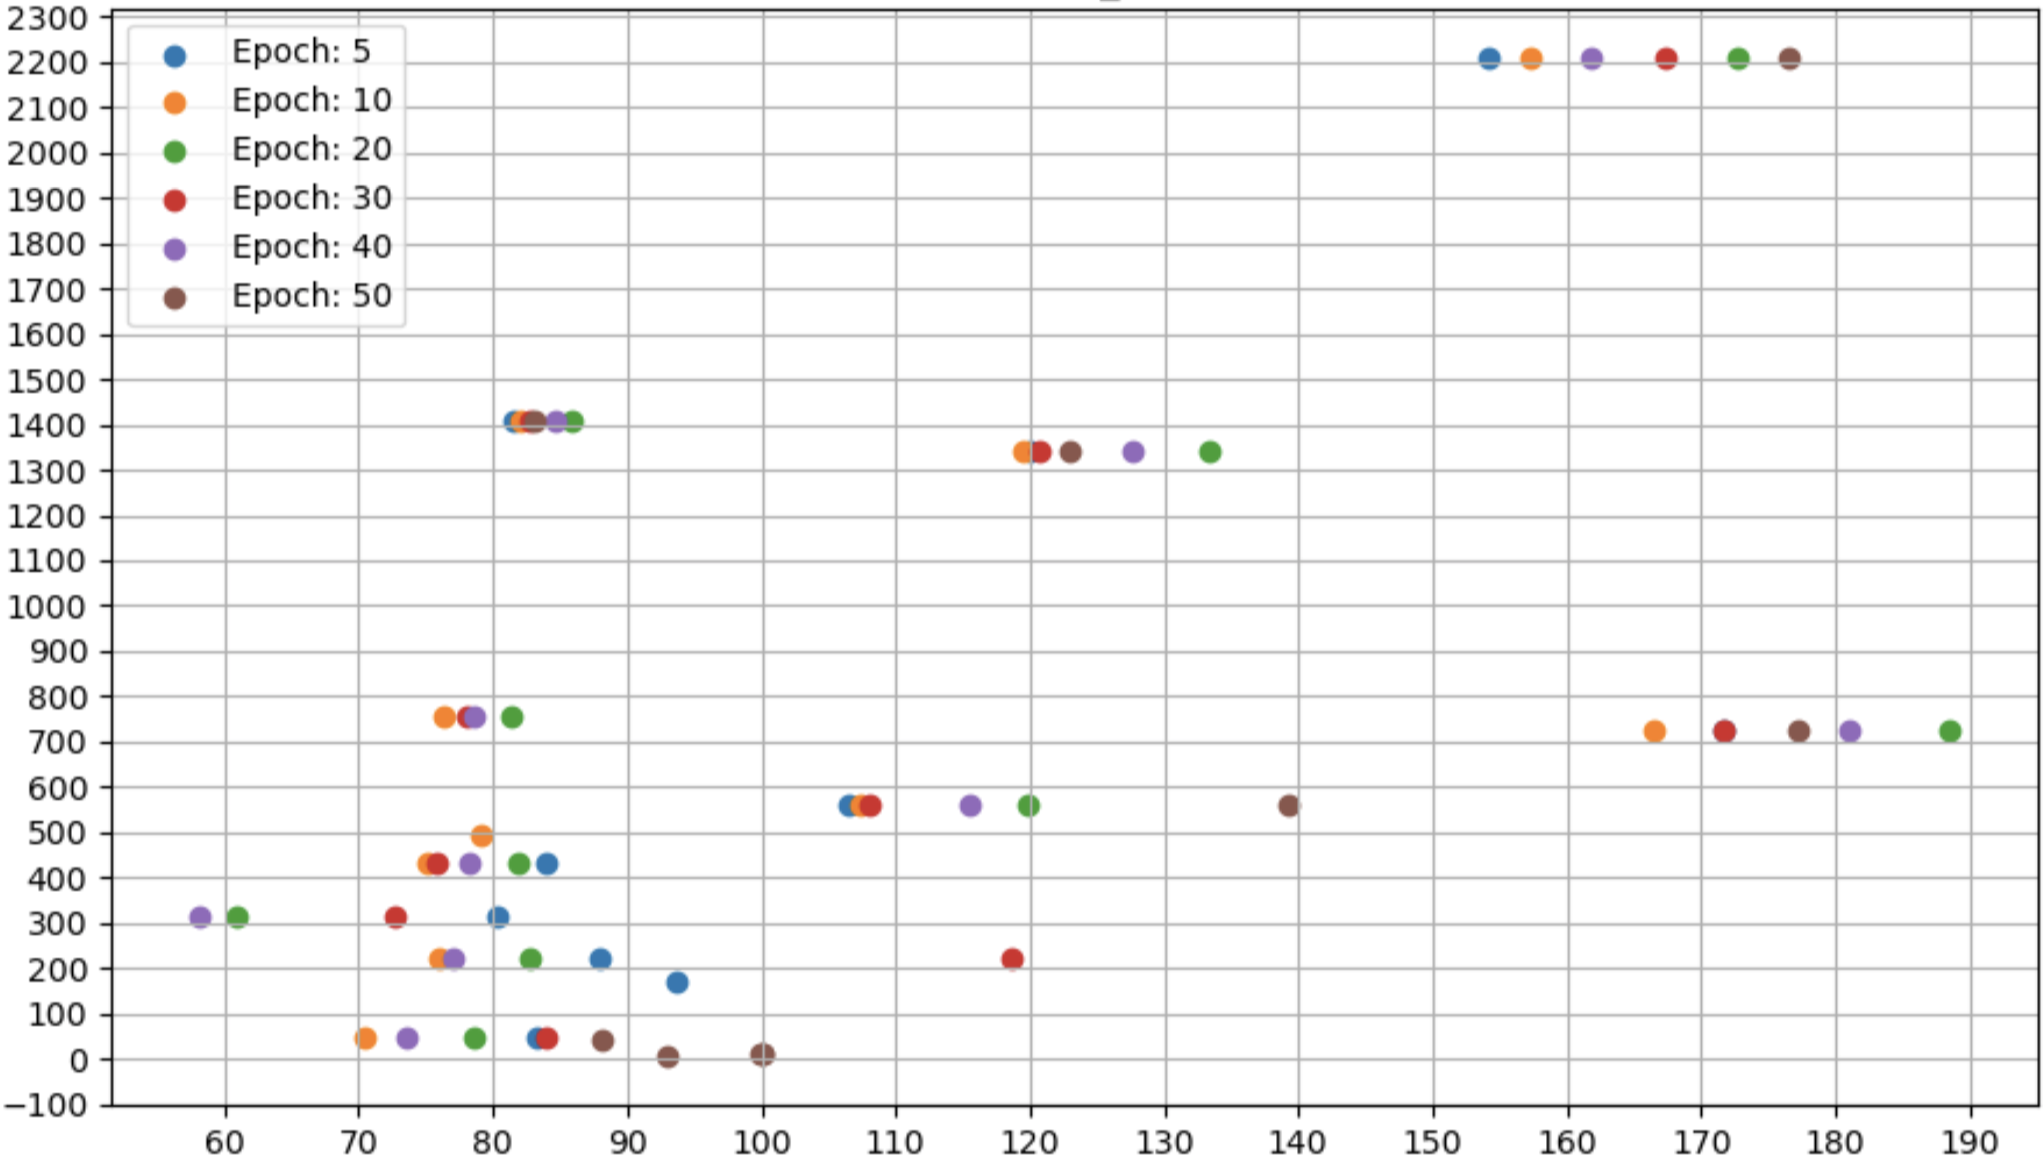
\includegraphics[width = \gws cm]{vgg16_sl_f.png}
	    \caption{VGG16}
        \label{fig:vgg16_sl_f}
        
     \end{subfigure}\\
     \caption{Inference time measured for model Resnet18 and Alexnet}
        \label{fig:sl_f_deep}
\end{figure}

For shallower networks, however, the situation is slightly more different. Fig. \ref{fig:sl_f_shallow} shows the slowest images identified in the models Resnet18 (Fig. \ref{fig:resnet18_sl_f}) and Alexnet (Fig. \ref{fig:alexnet_sl_f}). Differently from what we concluded before, these models show a much more precise response for images smaller than 500 kbs. We are in fact able to cluster the images by size, with the exception of very few outliers. In addition, we can also point out which number of epoch would yield faster predictions for the slowest images. For Resnet18, we can observe that the model trained with 40 epochs is among the fastest for most sizes, with very few exceptions. For alexnet, on the other hand, the fastest model is the one trained for only 10 epochs. This conclusion, however, does not take into account the accuracy that those models achieved. Using Fig. \ref{fig:inf_acc_resnet18} we can see that the same models, i.e. Resnet18 trained with 10 epochs, achieved one of the lowest accuracy rate over all (\textasciitilde90\%) and from Fig. \ref{fig:inf_acc_alexnet} we can extrapolate a similar conclusion for Alexnet trained with 10 epochs.(\textasciitilde80\%). \\
The best trade off between fast inference time and accuracy is achieved when both models have been trained with 50 epochs, however, in case of Resnet18, as we discussed before, this is also the number of epochs when the validation loss is bigger than the training loss, hence we found ourself in a situation of slight over-fitting. \\
\begin{figure}[h]
     \begin{subfigure}{0.5\textwidth}
	    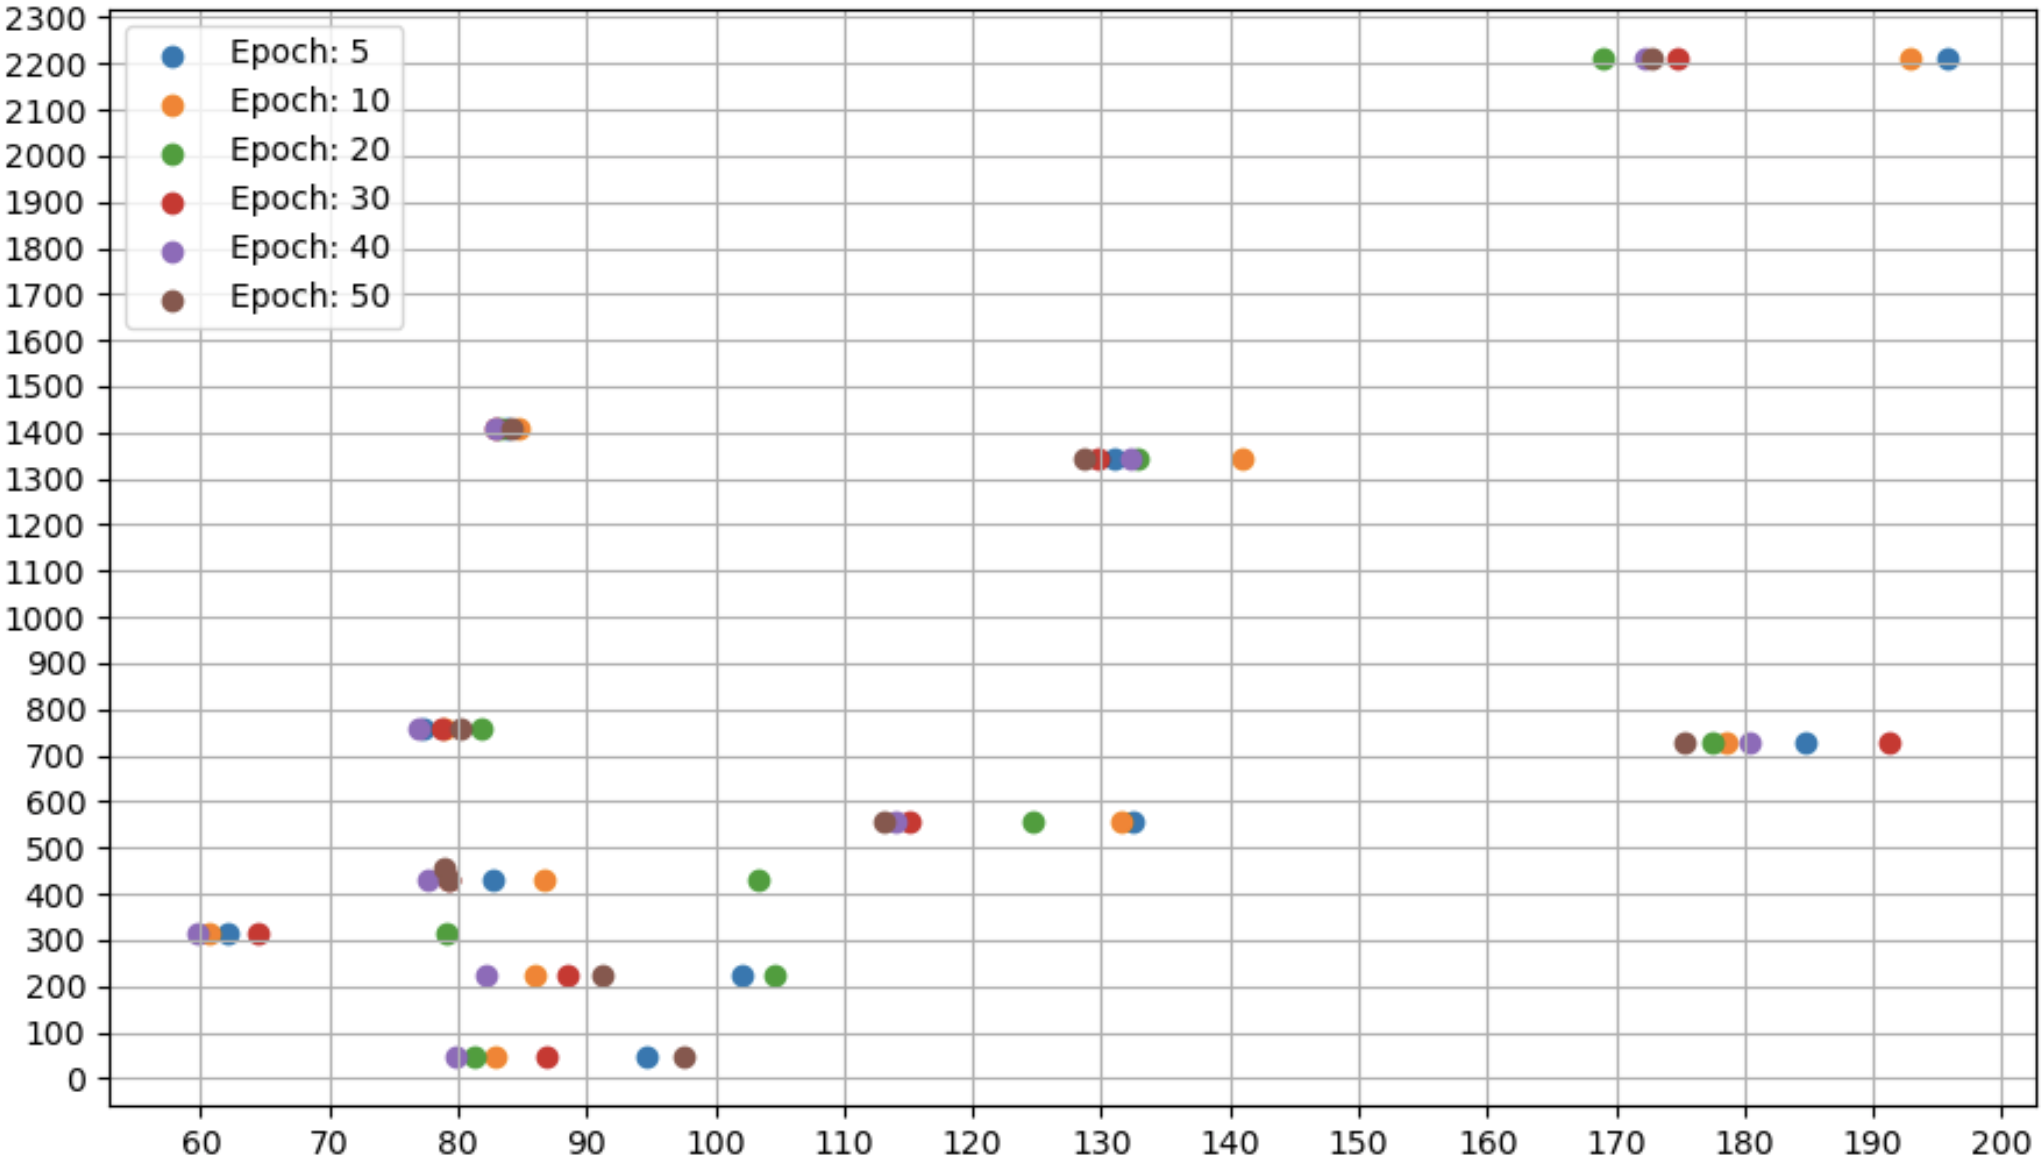
\includegraphics[width = \gws cm]{resnet18_sl_f.png}
	    \caption{Resnet18}
         \label{fig:resnet18_sl_f}
         
     \end{subfigure}
     \hfill
     \begin{subfigure}{0.5\textwidth}
	    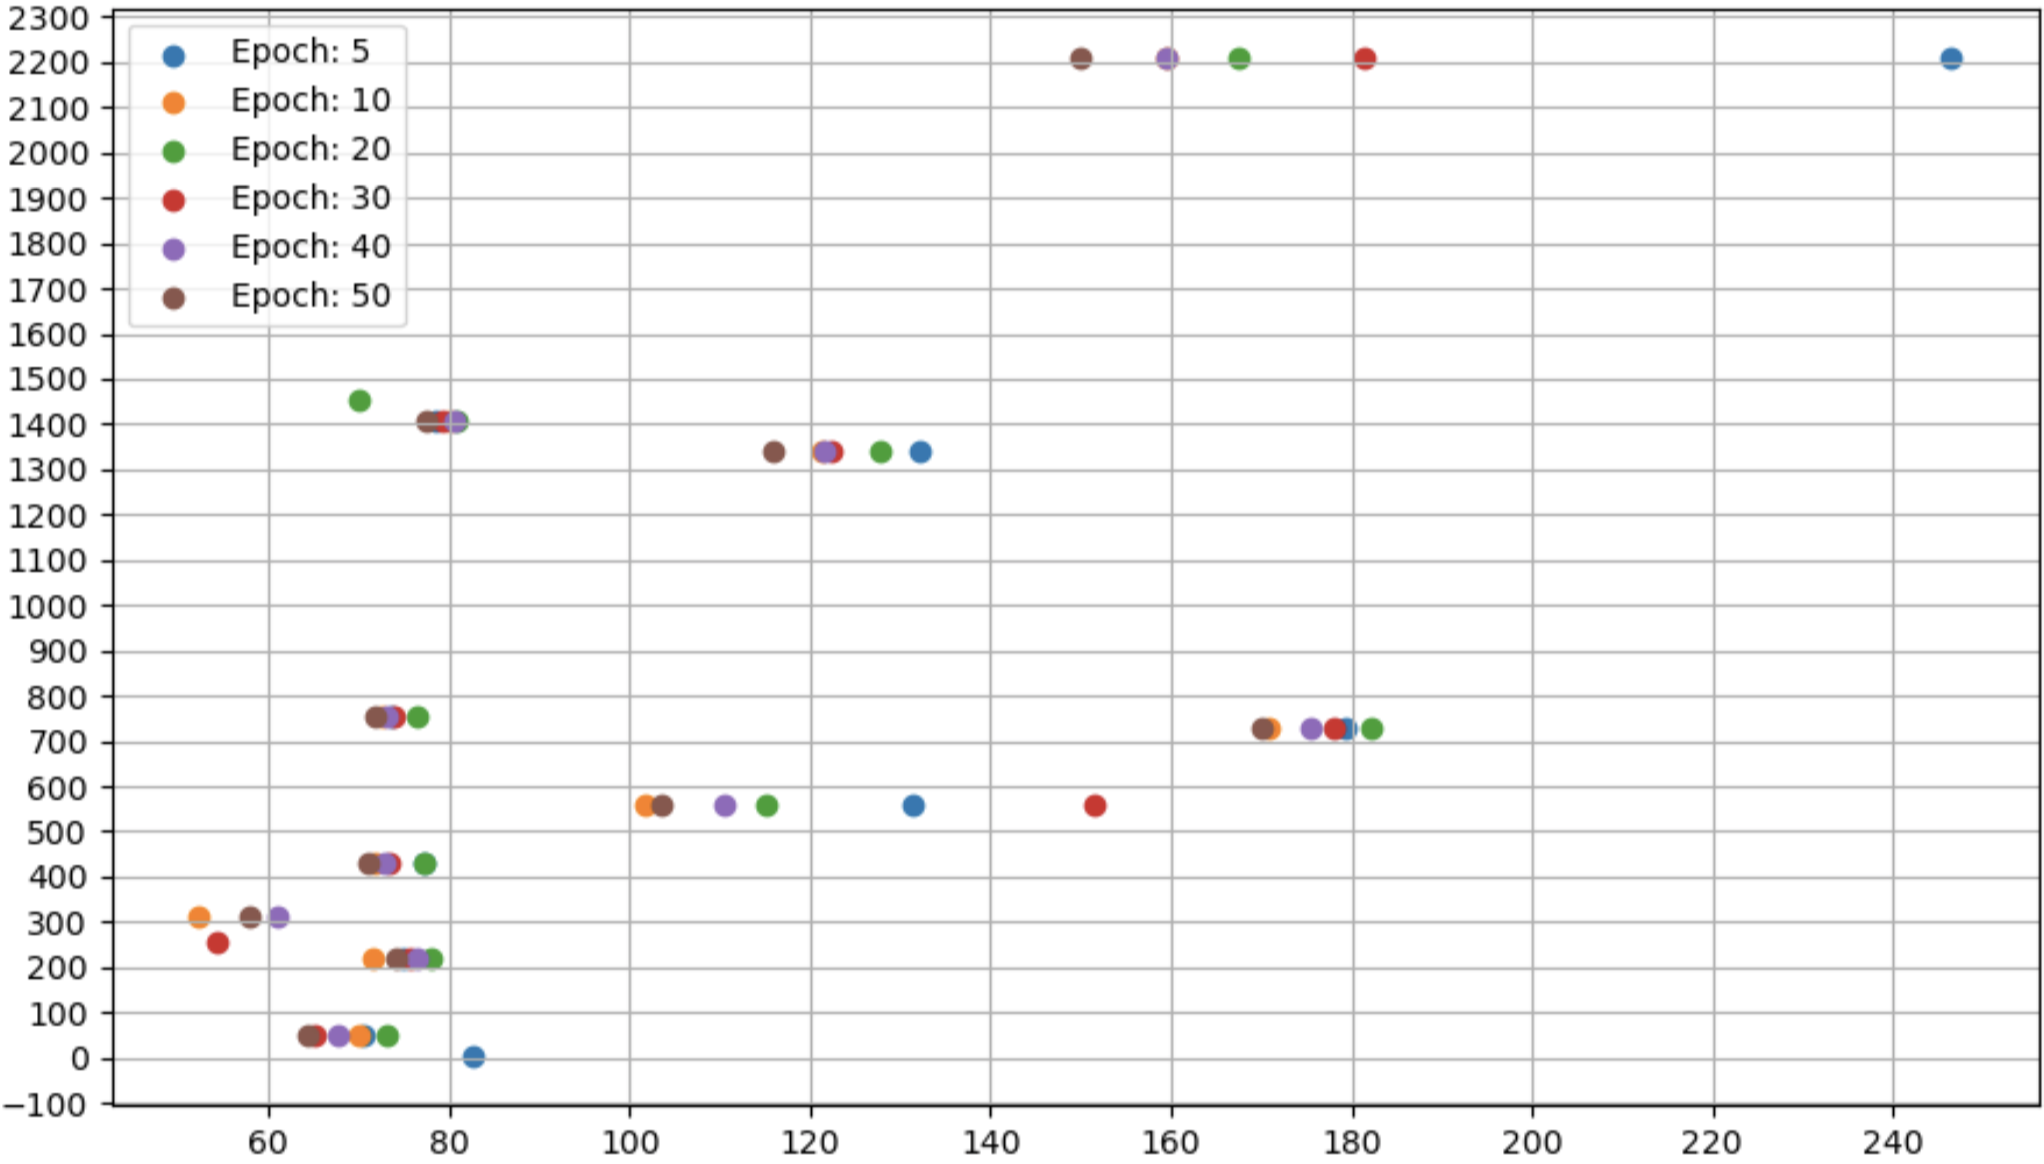
\includegraphics[width = \gws cm]{alexnet_sl_f.png}
	    \caption{Alexnet}
        \label{fig:alexnet_sl_f}
        
     \end{subfigure}\\
     \caption{Inference time measured for model Resnet18 and Alexnet}
        \label{fig:sl_f_shallow}
\end{figure}


Regardless of which number of epoch is better for this specific case, the purpose of our exploration is to identify correlation between certain characteristics. From these graphs we are able to find a correlation and to reason about it in order to tailor future applications. \\
In a real world implementation, if is is known that images with a certain size are going to be among the slowest is useful because it will influence the decision of which camera to mount on the devices sent to the fields. For example, knowing that images with a size of 700 kbs are going to take 200 to 220 ms to be classified will help model the time behaviour of these devices and give information to verify that they won't miss any deadline. Furthermore, if we are able to reason about the trade-off between inference time and accuracy we are also able to choose a suitable model for different requirements. For example, in case the highest accuracy possible is not a hard requirement, but we have a hard deadline to respect, we are able to identify which model and the amount of training necessary to respect those requirements. \\

A closer look to the list of slowest images reveals that there are pictures in common amongst all models (Fig. \ref{fig:slowest_files_all}). Using the tool we can investigate if those pictures present similarities that may explain why this is the case. The information collected from the pictures are shown in table 
\ref{tab:pictures_info}.

\begin{table}[htbp]
\centering
\begin{tabular}{ p{2cm} p{4cm}  p{2cm}  p{2cm}  }
 Picture n.& Dimensions(x,y) & DPI(x,y)&size(kb) \\
 \hline
1&(3888, 2187)&N/A& 727\\
2&(3018, 2585)&(300,300)&2209\\
3&(3000, 2019)&(300,300)&1341\\
4&(2003, 2003)&N/A&558\\
5&(1373, 1012)&(72,72)&1409\\
 \hline
\end{tabular}
\caption{Information collected from the slowest pictures}
\label{tab:pictures_info}
\end{table}

As already demonstrated by Fig. \ref{fig:size_inference_time_compared}, each of the five pictures has a size bigger than 500kb, i.e. they are amongst the heaviest pictures on the dataset. Furthermore, they are also amongst the pictures having the highest dimensions. Even though not available for all the pictures, table \ref{tab:pictures_info} also shows that the pictures have high DPI, which implies that these pictures have very high quality. 






%%%%%%%%%%%%%%%%%%%%%%%%%%%%%%%%%%%%%%%%%%%%%%%%
\section{Second Experiment}
In this section, we are going to analyse the performances of the models over the 'plant\_ seedlings \_v2' data-set. This dataset contains information taken from the agricultural field, we can therefore use the benchmarking tool to measure the metrics in a setting that reflects better a real-world use of the tool.\\
Similarly to the first experiment, the first metric we are going to analyse is training time. The tool run the test three times for 100, 200 and 50 epochs. 
We are going to start our analysis by studying the results obtained when trained for 100 epochs, which are shown in Fig. \ref{fig:seedlings_100_epoch_accuracy} and \ref{fig:seedlings_100_acc}. \\
As already encountered in the first experiment, Alexnet is the model that achieved the lowest accuracy overall reaching \textasciitilde86\% after 99 epochs. The highest accuracy has been achieved by Resnet101, peaking at \textasciitilde97\% after 66 epochs. Moreover, VGG16 and VGG19 achieved the same peak accuracy at \textasciitilde95\%, however VGG16 required 13 epochs less (43 compared to the 56 needed for VGG19). Similarly, Resnet18 and Resnet34 achieved comparable top accuracies at  94.39\% and 94.48\% respectively, however Resnet34 required considerably less time to reach this number peaking after 62 epochs, while Resnet18 achieved this number when the training cycle was almost done, namely after 96 epochs. An overview of the performances of all the models can be seen in table \ref{tab:performances_seeds}. 
\begin{table}[htbp]
\centering
\begin{tabular}{ p{2cm} p{4cm} p{3cm} p{3cm} p{2cm}  }
 Model& Top Accuracy (\%) & Epochs needed &Average Time (s)&Total Time (s)\\
 \hline
Resnet18&94.39&96&7&747\\
Resnet34&94.48&62&9&876\\
Resnet50&96.65&67&14&1439\\
Resnet101&97.01&66&21&2101\\
Resnet152&96.56&98&29&2851\\
Alexnet&85.88&63&7&705\\
VGG16&95.20&43&17&1743\\
VGG19&95.20&56&20&1952\\
 \hline
\end{tabular}
\caption{Performances of the models trained with the 'plant\_seedlings\_v2' dataset for 100 epochs}
\label{tab:performances_seeds}
\end{table}\\



Fig. \ref{fig:seedlings_100_epoch_accuracy} shows the response of all models during the training based on the epoch used for training. Similarly to the first experiment, the response of the model shows that within the first ten epochs the accuracy increases quickly and tends to stabilize afterwards, increasing slowly over time. However, contrary to the first experiment, here we can observe a more compact graph, meaning that the all the models except Alexnet achieved accuracies not far off from each other.
As a matter of fact, the difference in accuracy between the highest performing model (Resnet101) and the lowest performing model (Resnet18) was only 3\%.  
\begin{figure}[h]
       \centering 
	    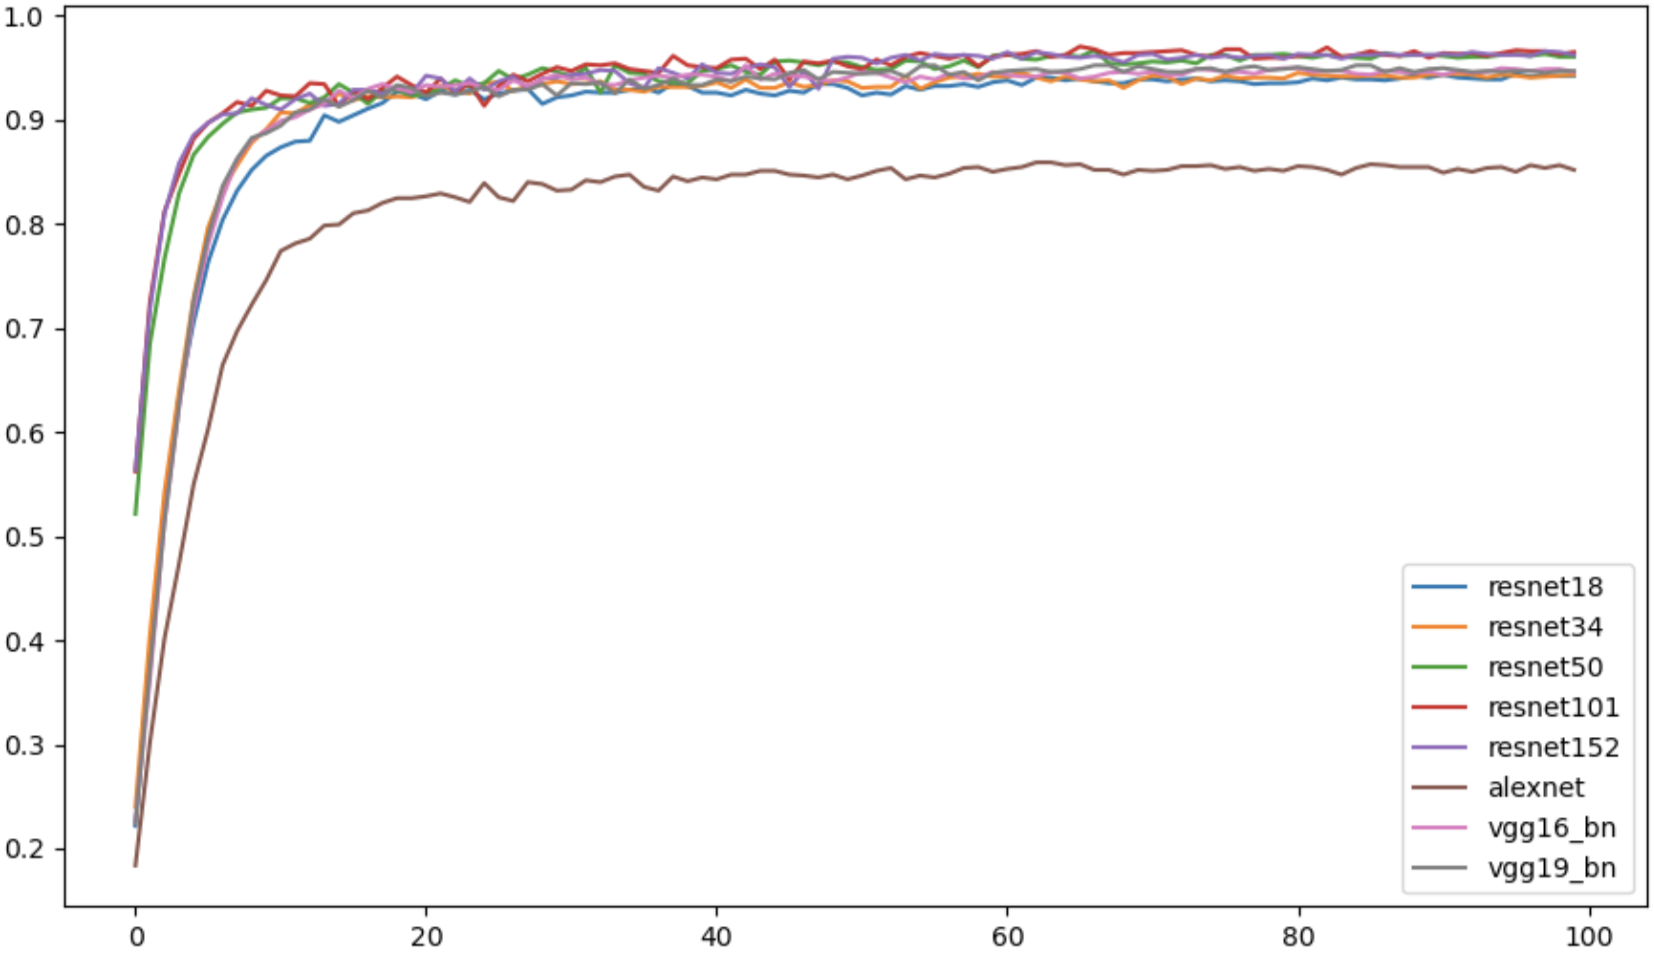
\includegraphics[width = 11 cm]{seedlings_100.png}
        \caption[Accuracy achieved when training for 100 epochs]{Accuracy achieved when training for 100 epochs. The x axis is the number of epochs, while the y axis is the accuracy achieved}
         \label{fig:seedlings_100_epoch_accuracy}
\end{figure}

Fig. \ref{fig:seedlings_100_acc}, on the other hand, depicts the accuracy graphed over training time. Alexnet took the least amount of time to finish the training cycle (747 seconds), however Resnet18 took only \textasciitilde40 seconds more and reached a far better accuracy(94\% compared to 85\%). Resnet152 took 47 Minutes and 30 Seconds (2851 seconds) to complete the test and is the model that required the most time. \\
\begin{figure}[h]
       \centering 
	    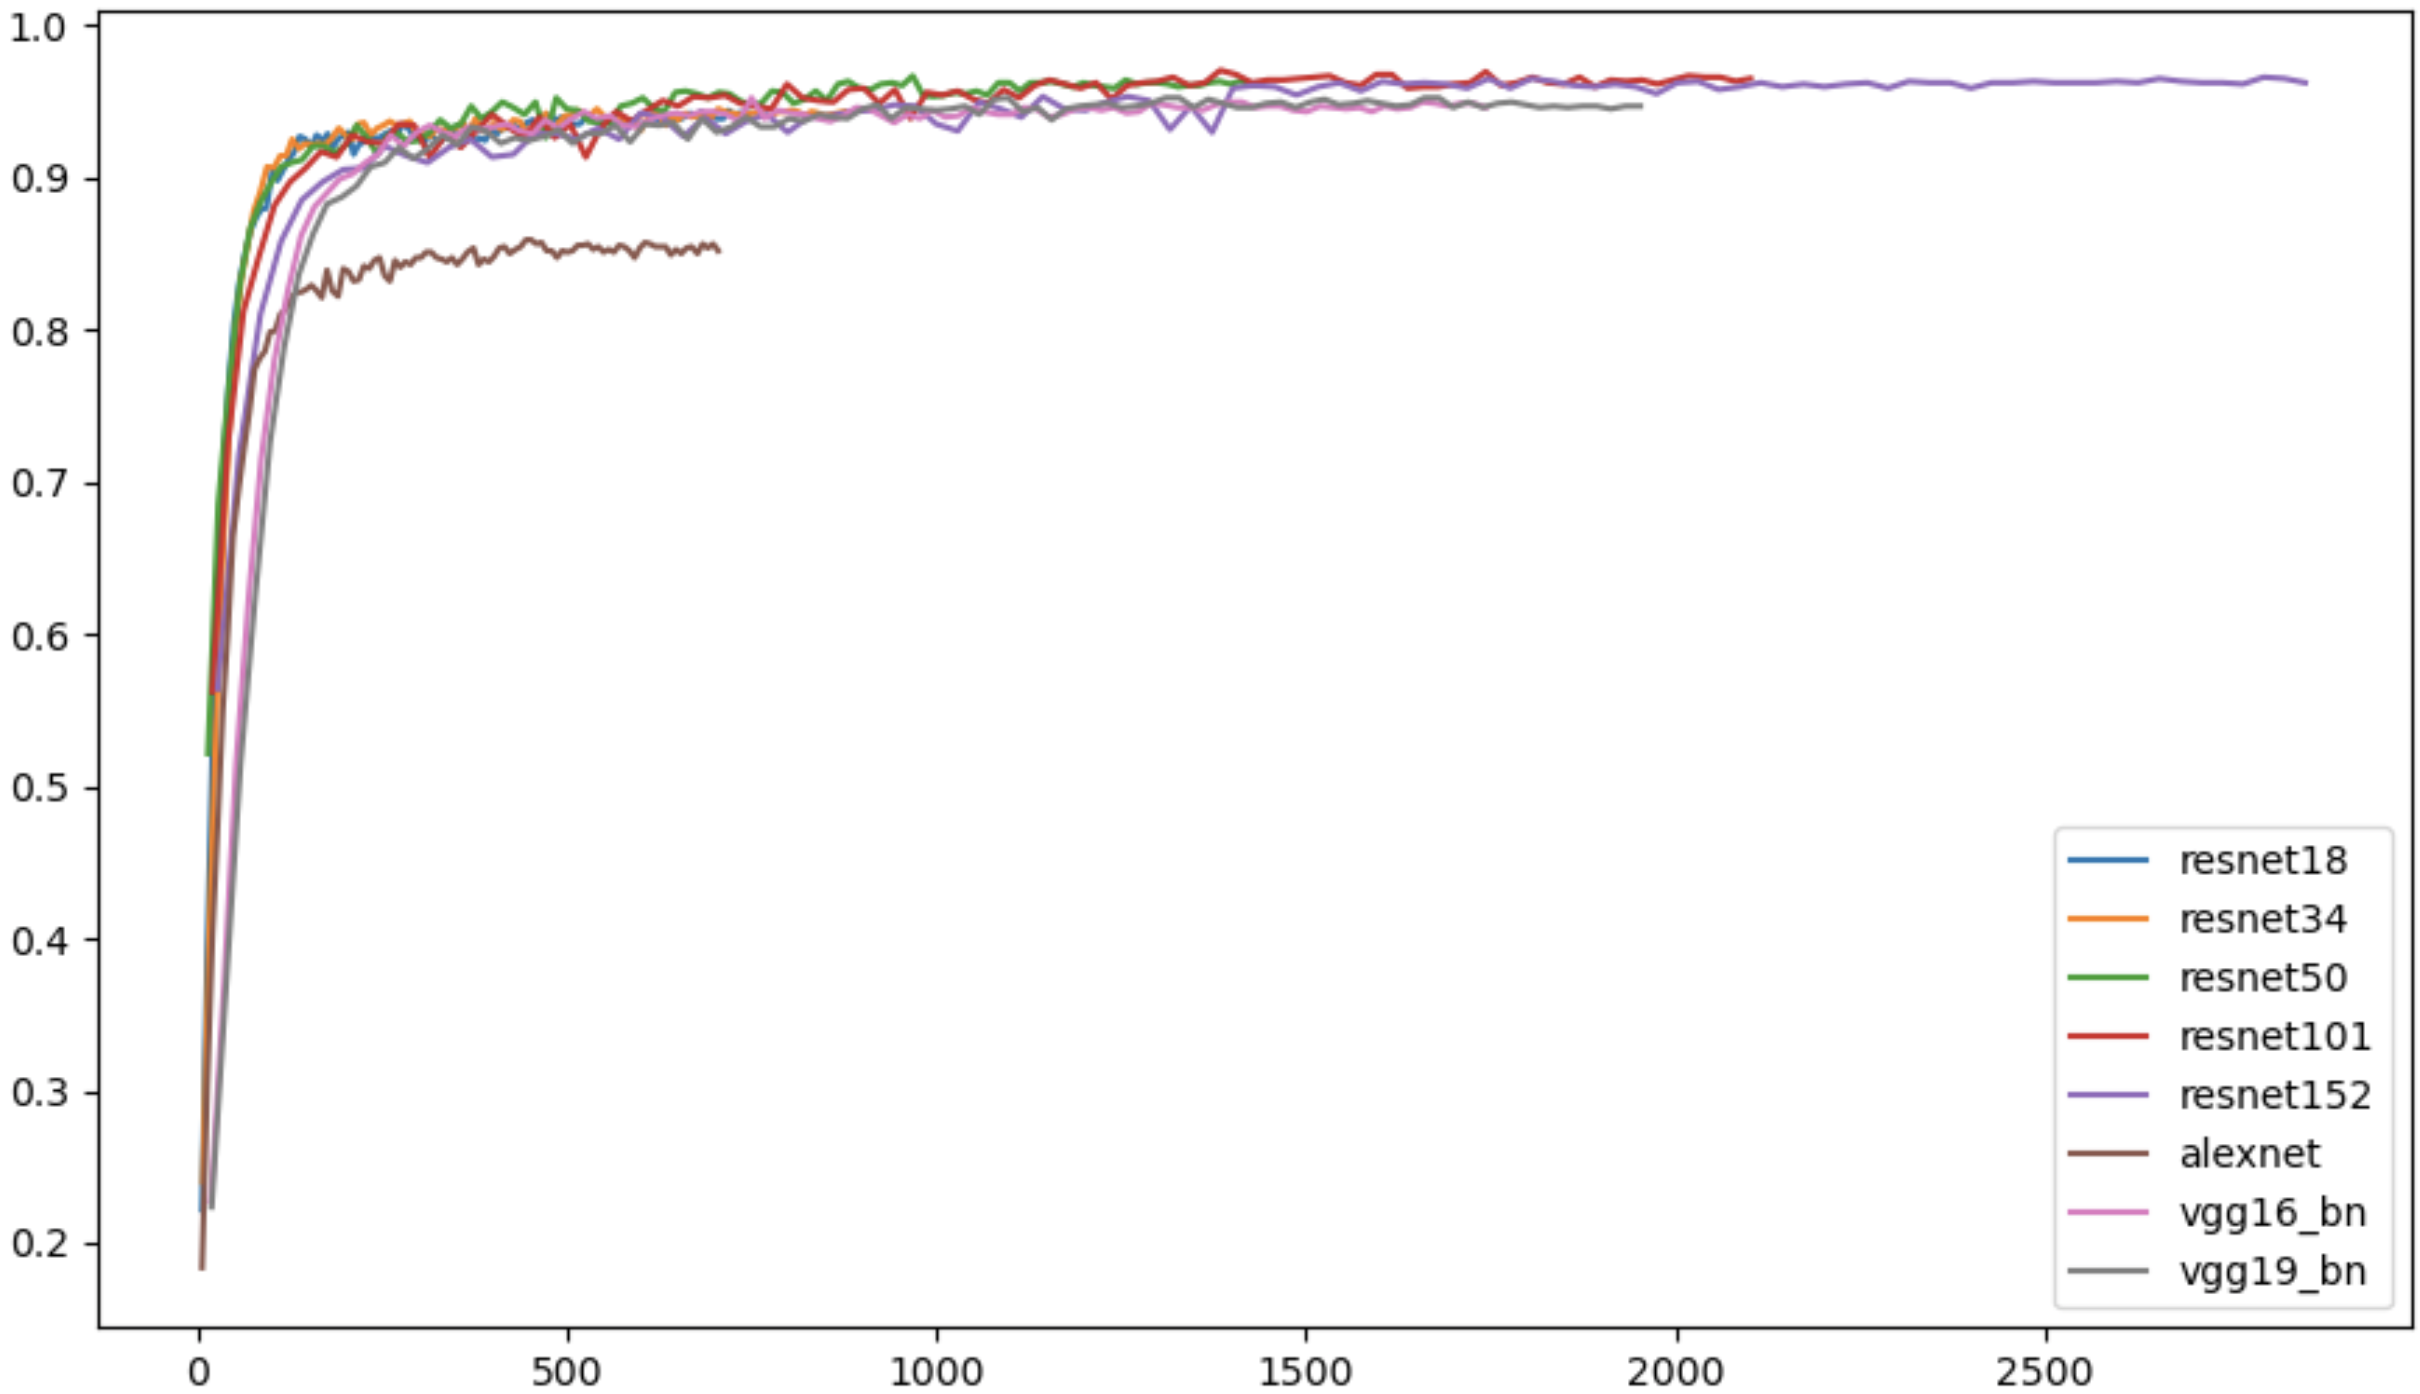
\includegraphics[width = 12 cm]{seedlings_100_acc.png}
        \caption[Accuracy achieved when training for 100 epochs in relation with training time]{Accuracy achieved when training for 100 epochs in relation with training time. The x axis is the training time in seconds, while the y axis is the accuracy achieved}
         \label{fig:seedlings_100_acc}
\end{figure}

\begin{figure}[h]
\begin{subfigure}{0.5\textwidth}
	    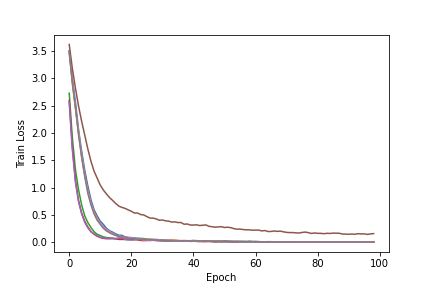
\includegraphics[width = \gws cm]{epoch_train_loss_seeds_100.png}
	    \caption{Training Loss calculated over 100 epochs}
        \label{fig:train_loss_seeds_100}
     \end{subfigure} \hfill
     \begin{subfigure}{0.5\textwidth}
	    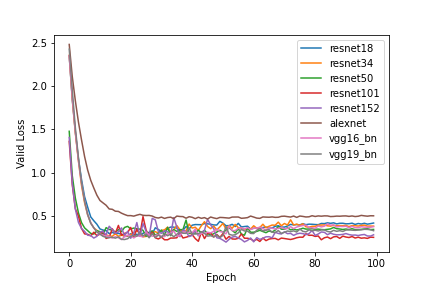
\includegraphics[width = \gws cm]{epoch_valid_loss_seeds_100.png}
	    \caption{Validation Loss calculated over 100 epochs}
         \label{fig:valid_loss_seeds_100}
     \end{subfigure}
     
     \caption{Training loss and validation loss of all models calculated over 100 epochs}
        \label{fig:tran_valid_loss_seeds_100}
        
      
\end{figure}

In Fig. \ref{fig:tran_valid_loss_seeds_100}, we can analyse the loss calculated for the models during the training. As shown in Fig. \ref{fig:train_loss_seeds_100}, all the models except Alexnet reached 0 loss within the first 30 epochs. This means that theoretically the models learned the data-set perfectly within the first 20 epochs. Usually, when the training loss is 0, we are excepting a situation of over-fitting and it would be proven by a high validation loss. We can study the validation loss of the models in Fig. \ref{fig:valid_loss_seeds_100}. From their response, we can observe that the validation loss does not increase drastically like we saw in the first experiment. On the contrary, we can see in table \ref{tab:difference_val_tra_loss} that the difference between validation loss and training loss rarely is more than 0.4. Furthermore, the curve seems to be quite stable, especially for shallower networks, and the validation loss tends to increase slowly. \\


\begin{table}[h]
\centering
        \begin{tabular}{ c c  }
                 Model&Difference\\
                 \hline
                   Resnet18&0.42\\
                    Resnet34&0.38\\
                    Resnet50&0.35\\
                    Resnet101&0.25\\
                    Resnet152&0.28\\
                    Alexnet&0.34\\
                        VGG16&0.38\\
                    VGG19&0.33\\
                    \end{tabular}
                    \caption{Difference between validation loss and train loss after 100 epochs }                   
                     \label{tab:difference_val_tra_loss}
     \end{table} 


For example, we can analyse the trend for the model which reached the highest accuracy overall, namely Resnet101, shown in Fig. \ref{fig:epoch_valid_loss_resnet101}. As shown in table \ref{tab:difference_val_tra_loss}, the difference at the end of the training is 0.25. Furthermore, as we suspected before, the training loss approaches zero within the first 30 epochs, while the validation loss remains stable for the entire training process, with some spikes around the 30 epochs. Furthermore, the validation loss becomes higher than the training loss around 10 epochs.\\
We can observe in the response of Resnet152 (Fig. \ref{fig:epoch_valid_loss_resnet152}) a similar behaviour. The training loss approaches once again zero around the 30 epochs and becomes smaller than the validation loss around 10. Although the validation loss tends to stabilize for this model as well, the graph shows a less stable behaviour with more fluctuations between 20 and 50 epochs. \\
\begin{figure}[h]
\begin{subfigure}{0.5\textwidth}
     \centering
	    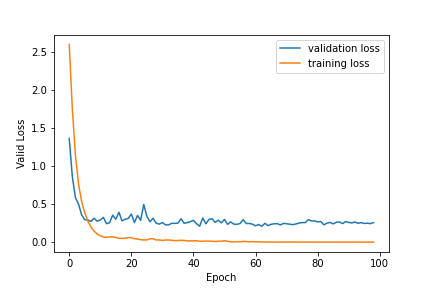
\includegraphics[width = \gws cm]{epoch_valid_loss_resnet101.png}
\caption{Validation loss and training loss for Resnet101 over 100 epochs}\label{fig:epoch_valid_loss_resnet101}
     \end{subfigure}
\begin{subfigure}{0.5\textwidth}
     \centering
	    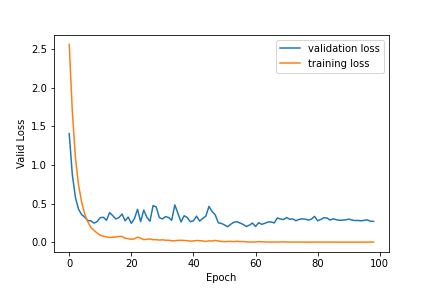
\includegraphics[width = \gws cm]{epoch_valid_loss_resnet152.png}
\caption{Validation loss and training loss for Resnet152 over 100 epochs}\label{fig:epoch_valid_loss_resnet152}
     \end{subfigure}  
     \caption{Training loss and validation loss of Resnet101 and Resnet152 over 100 epochs}
        \label{fig:tran_valid_loss_seeds_res_100}
\end{figure}



As we already did for the first experiment, we can use the tool to test the inference time of each model. We are going to use a data-set composed of \textasciitilde120 pictures taken from the original dataset. These pictures were taken before starting the process, therefore they have not been used for training. \\
The results are shown in Fig. \ref{fig:inf_time_epoch_seeds}. Fig. \ref{fig:inf_acc_models_seeds} shows the inference time based on the accuracy, while figure \ref{fig:inf_epoch_models_seeds} shows the inference time based on the epoch used to train. \\
From Fig. \ref{fig:inf_acc_models_seeds} we can start to observe some rather interesting properties. For each model, as they achieve accuracy less than 88\%, the inference time is rarely measured to be more than 60 ms with only 2 exceptions (\textasciitilde100ms and \textasciitilde390ms). Furthermore, the only model that achieved an accuracy smaller than \textasciitilde82\% is Alexnet\footnote{The whole results can be seen in Fig. \ref{fig:accuracy_inferencetime_seedlings}}.
\begin{figure}[h]
     \begin{subfigure}{0.5\textwidth}
	    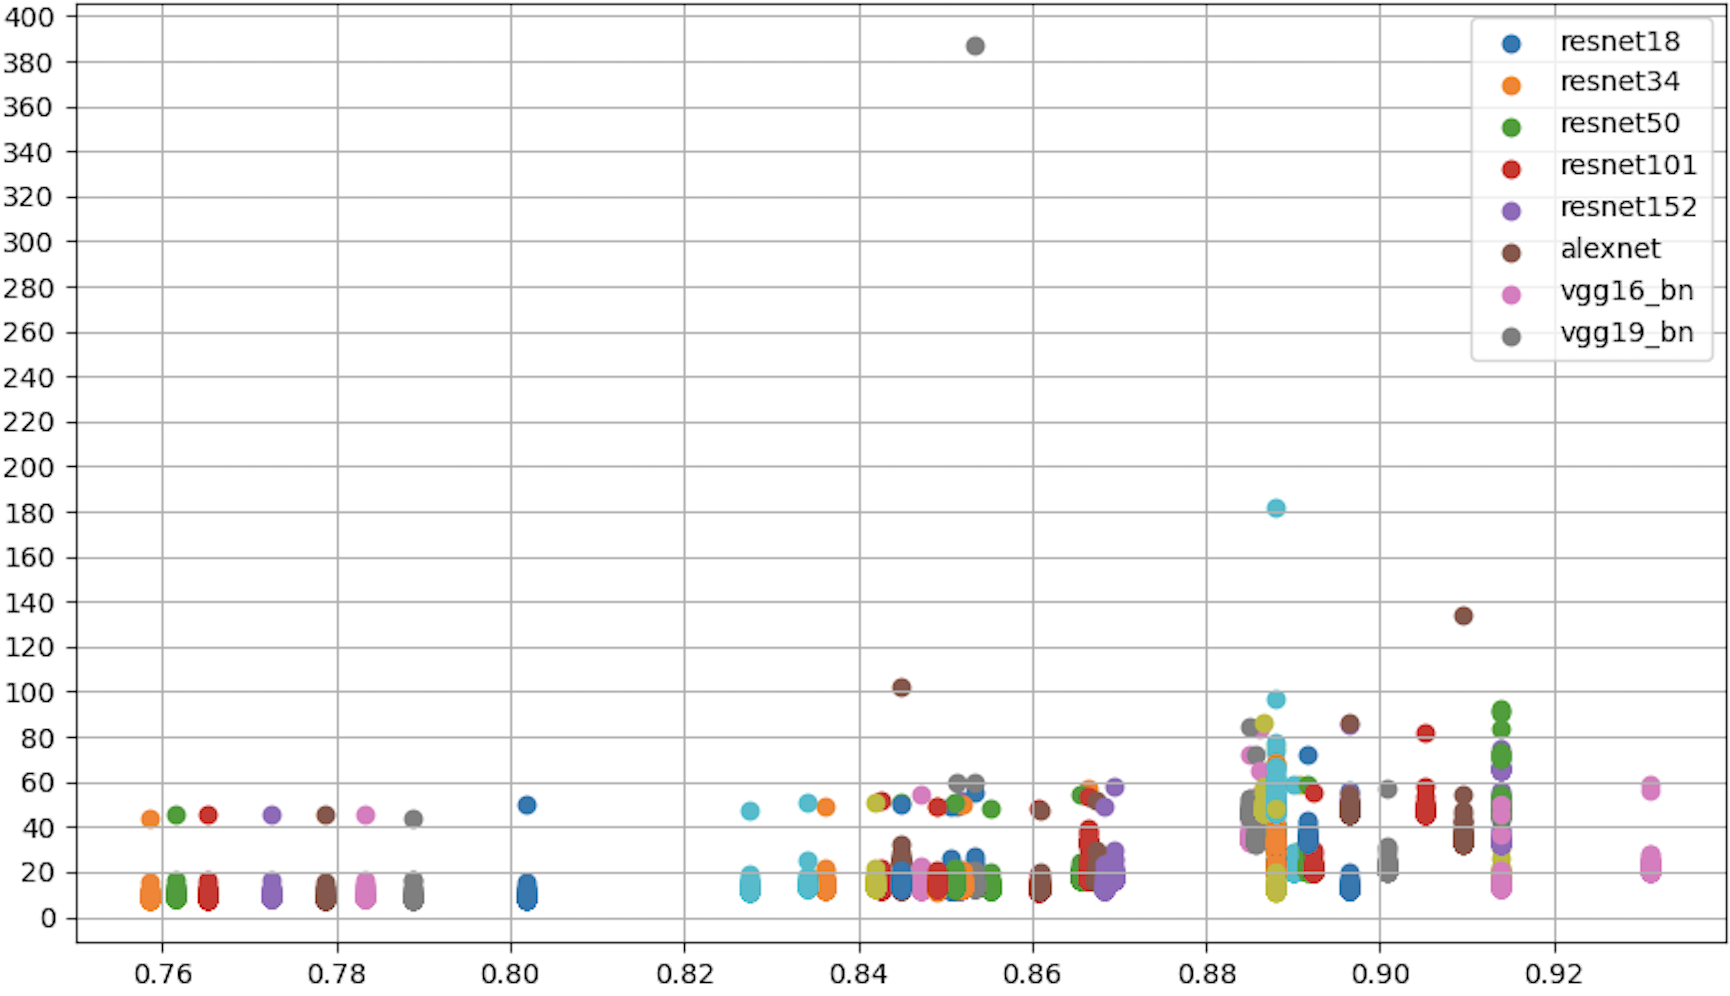
\includegraphics[width = \gws cm]{inf_acc_models_seeds.png}
	    \caption{Based on accuracy}
         \label{fig:inf_acc_models_seeds}
     \end{subfigure}
     \hfill
     \begin{subfigure}{0.5\textwidth}
	    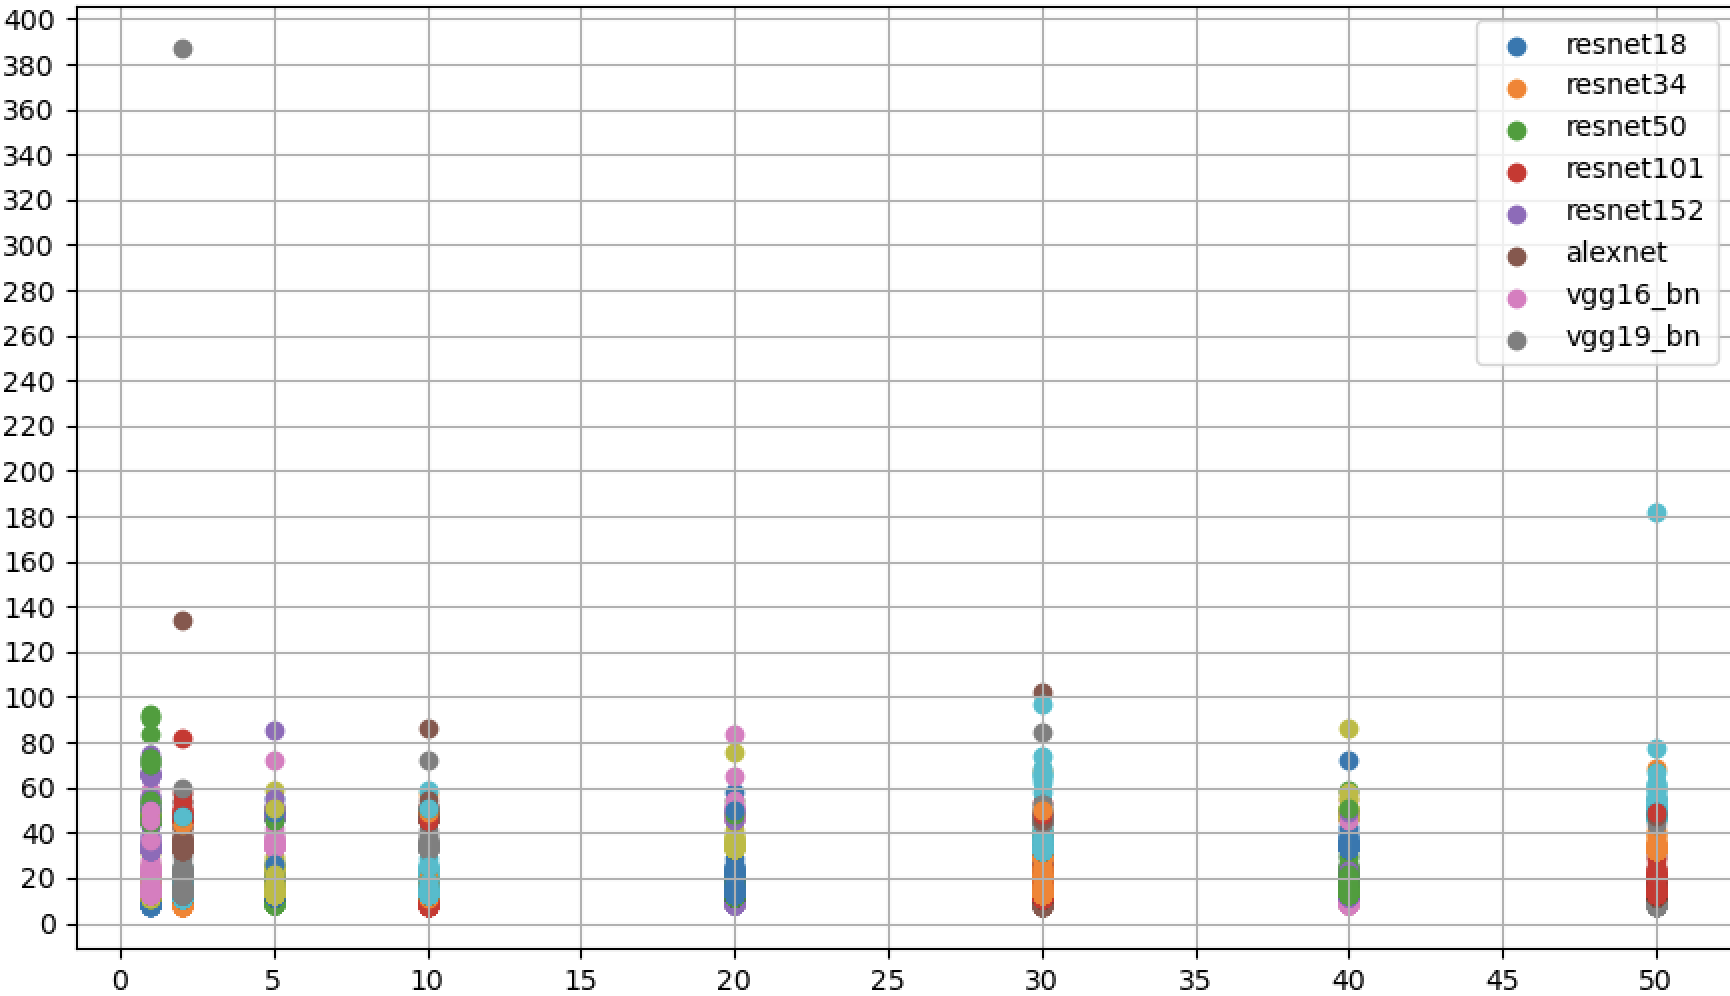
\includegraphics[width = \gws cm]{inf_epoch_models_seeds.png}
	    \caption{Based on the epoch}
        \label{fig:inf_epoch_models_seeds}
     \end{subfigure}\\
     \caption[Inference time measured for each model]{Inference time measured for each model using dataset discussed previously. The inference time is in milliseconds, while the accuracy for Fig. \ref{fig:inf_time_accuracy}is the percentage of correct predictions.}
        \label{fig:inf_time_epoch_seeds}
\end{figure}


For accuracies over 88\%, although the behaviour of the models seems to be less compact, the inference time rarely measures more than 100 milliseconds, with only two outliers(\textasciitilde135ms and \textasciitilde180s).\\
From Fig. \ref{fig:inf_epoch_models_seeds} we can see that, with the exception of the outliers we identified before, the number of epochs that measured the highest value for inference is 30. As a matter of fact, when trained for different numbers of epochs, the models never require more than 100 milliseconds to process the images. 
\begin{figure}[h]
     \begin{subfigure}{0.5\textwidth}
	    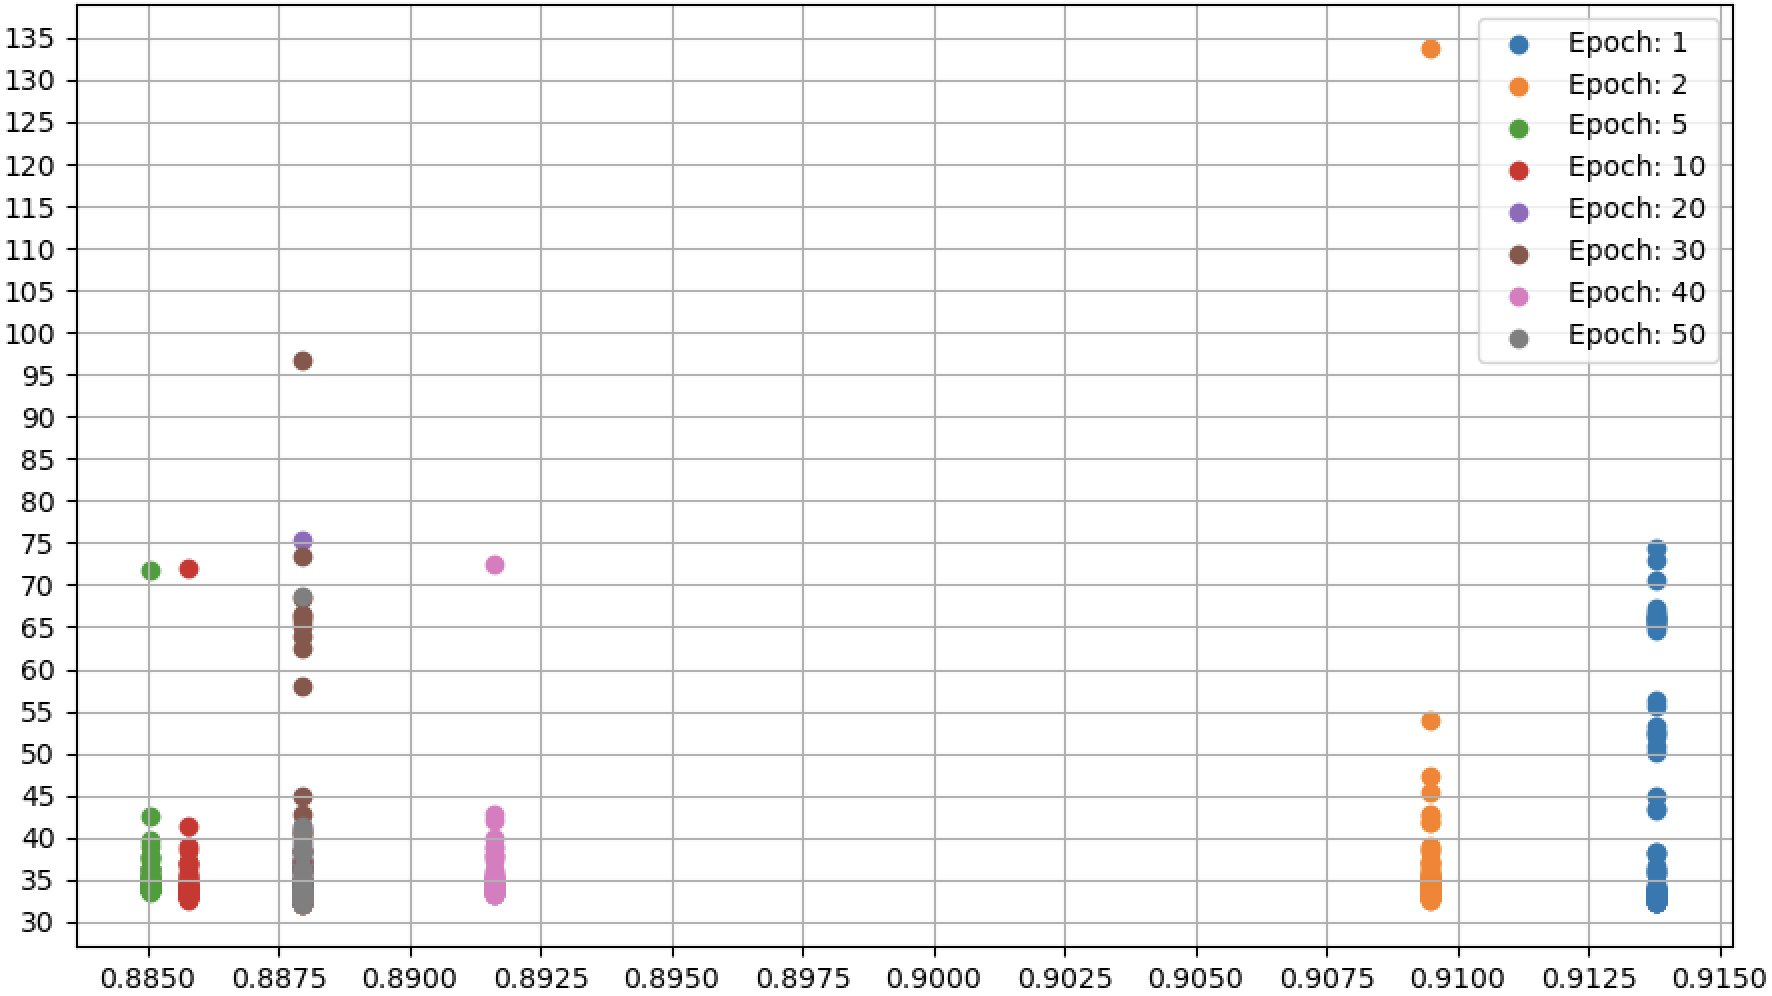
\includegraphics[width = \gws cm]{inf_resnet101_seeds.png}
	    \caption{Resnet101}
         \label{fig:inf_resnet101_seeds}
     \end{subfigure}
     \hfill
     \begin{subfigure}{0.5\textwidth}
	    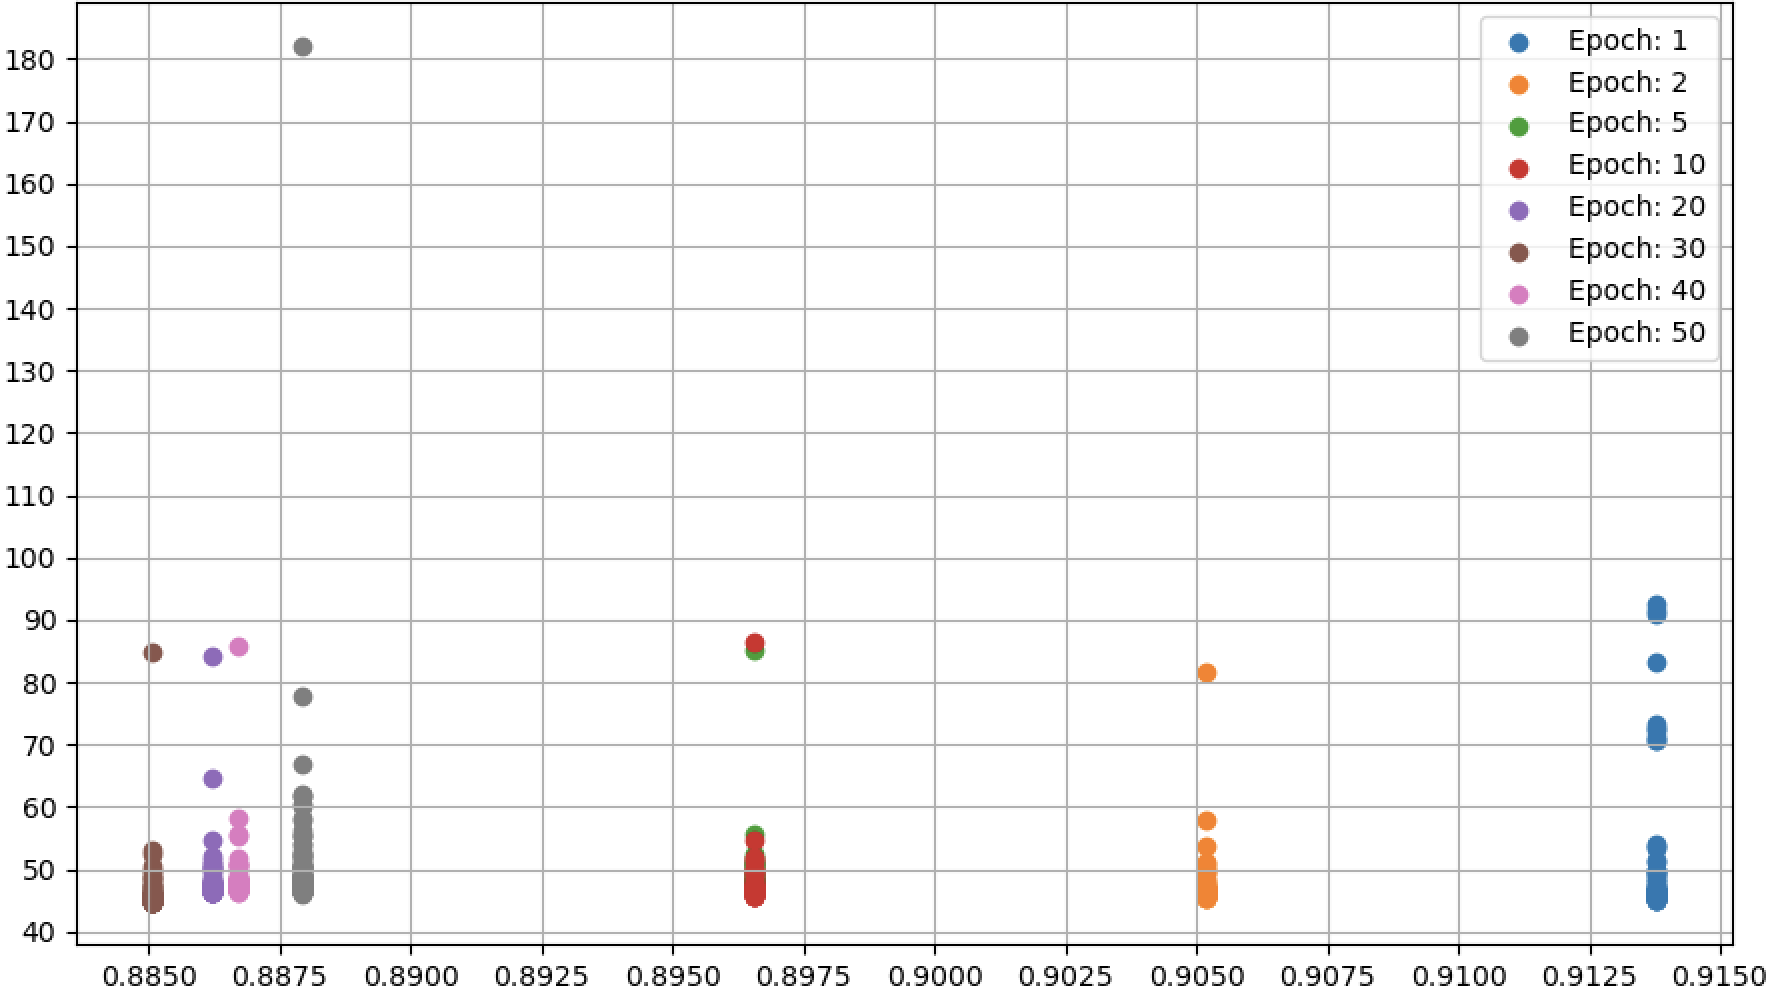
\includegraphics[width = \gws cm]{inf_acc_152_seeds.png}
	    \caption{Resnet152}
        \label{fig:inf_acc_152_seeds}
     \end{subfigure}\\
     \caption[Inference time measured for Resnet101 and Resnet152]{Inference time measured for Resnet101 and Resnet152. The inference time is in milliseconds, while the accuracy is the percentage of correct predictions.}
        \label{fig:inf_time_epoch_seeds}
\end{figure}



A closer investigation of the individual performance of each model shows further interesting aspects. For the purpose of this experiment, we are going to analyse only Resnet101 and Resnet152, whose behaviour is shown in Fig. \ref{fig:inf_resnet101_seeds} and Fig. \ref{fig:inf_acc_152_seeds} respectively. For both model, we can see that the highest accuracy is achieved when trained for only one (\textasciitilde91\% for both) and two epochs (slightly lower of 91\% for Resnet18 and \textasciitilde90\% for Resnet152). For the other epoch, the accuracy achieved was consistently lower than 90\%. \\
In the case of Resnet101, the fastest training time has been achieved when trained for ten and five epochs, with an inference time over 45 milliseconds only in two occasions. Although the fastest, the model trained with these epochs also achieved the lowest accuracy. The slowest inference time has been achieved when the model has been trained for two epochs, with an inference as high as 135 milliseconds. However, the model achieved the worst performance when trained for 30 epochs. As a matter of fact, even though when trained for two epochs it measured the lowest inference time, this happened only in one case, while, when trained for 30 epochs, for a considerable amount of pictures, the inference time was in a range between 57 and 95 milliseconds. \\
Resnet152, on the other hand, showed more consistent results, with an inference time being in the range of 40 to 90 milliseconds for all epochs with the exception of one case where it reached 180 milliseconds. The fastest inference time for this model is measured when the model has been trained for 20 epochs.\\
From this investigation we can conclude that the performances of these two models are quite comparable when it comes to inference. Both in terms of inference time and accuracy achieved, the two models show similar results, however for different levels of training. \\
For example, in case of Resnet152, with a training time of 580 seconds (20 epochs), we will obtain a model that can make predictions in a range between 45 and 85 milliseconds with an accuracy of \textasciitilde89\%. In the case of Resnet101, we can obtain similar results (prediction time between 70 and 30 milliseconds with an accuracy of \textasciitilde89\%) with a training time of 210 seconds (10 epochs). \\

\begin{figure}[h]
       \centering 
	    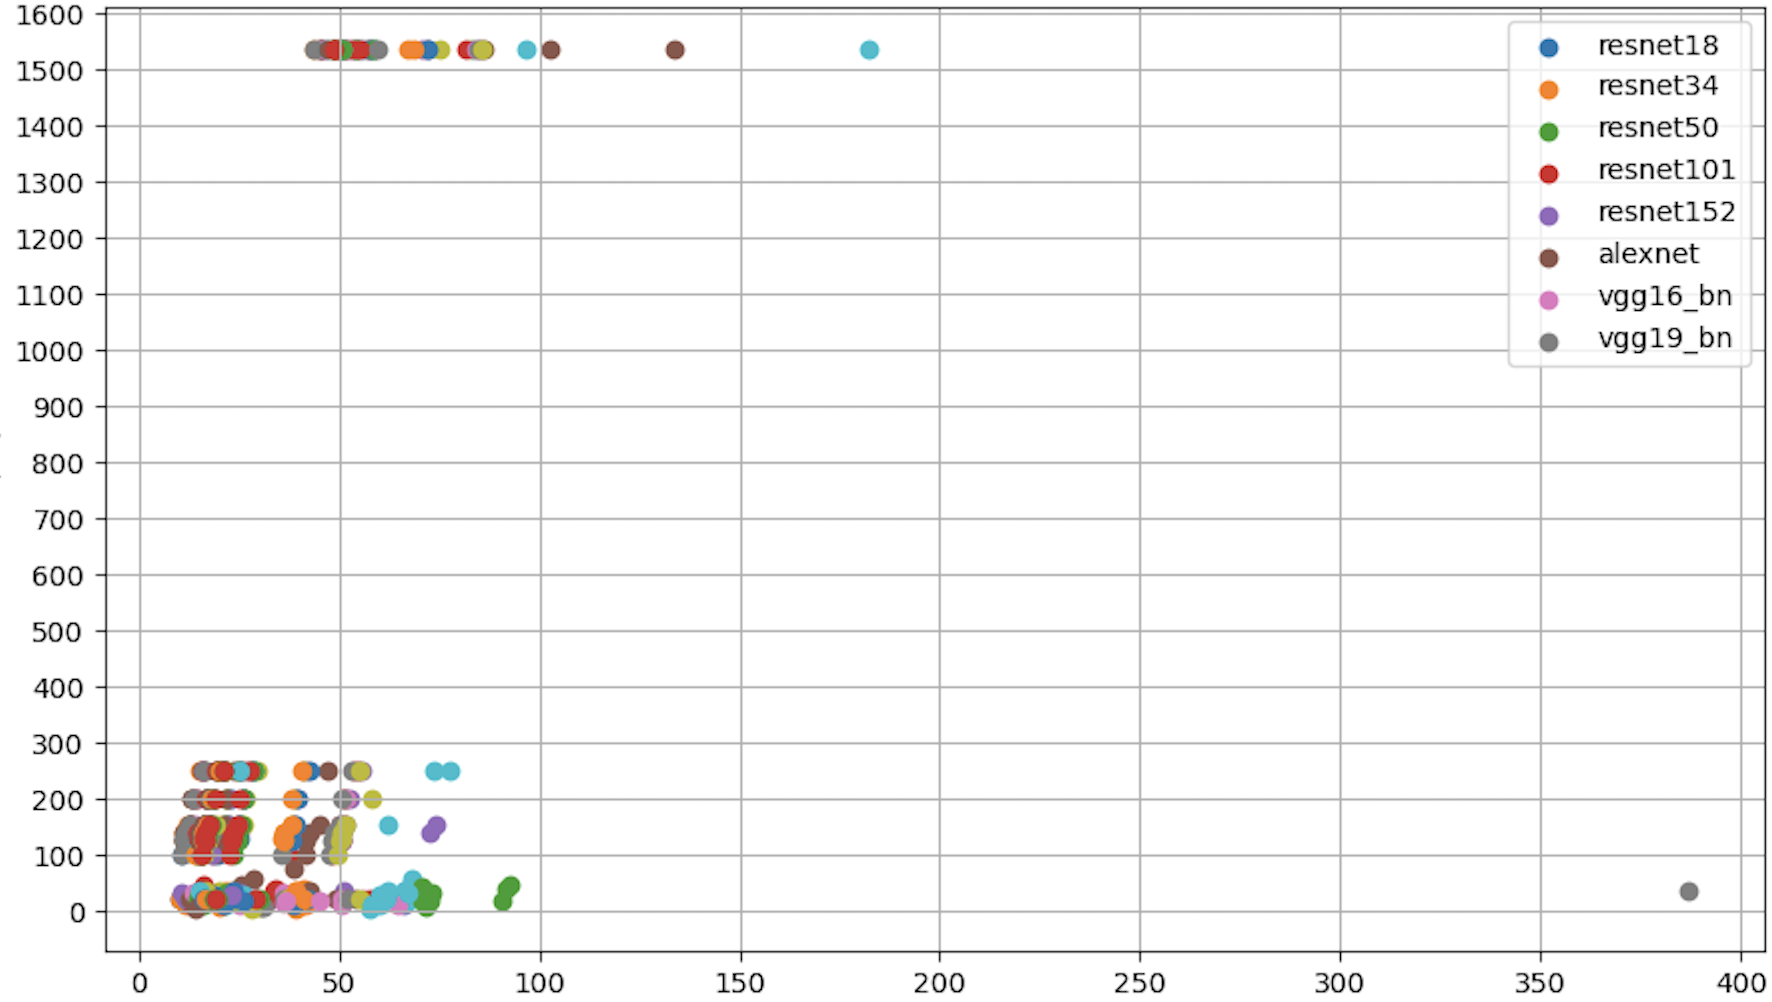
\includegraphics[width = 14 cm]{inf_size_seeds.png}
        \caption[Size of the images over inference time for the seedlings dataset]{This graph shows the size in kb (y axis) of the ten slowest images over the time taken to be processed (x axis)}
         \label{fig:inf_size_seeds}
\end{figure}


As we already performed for the first experiment, we can also run the tool discover which pictures took the most amount of time to be processed. Fig. \ref{fig:inf_size_seeds} shows the ten slowest image for each model graphed based on their sizes. \\
The graph shows a rather compact and stable behaviour, with the slowest time measured for images having a size bigger than 1500 kb. \\
For pictures of more than 100 kb and less than 300 kb, the inference time is between 0 and 100 ms, with each model performing rather similarly. \\
For this experiment, both for training and for testing inference, we used a dataset with images having rather similar size and resolution, therefore this analysis is not as valuable as the one we did for the first experiment. \\
However, we can run the tool to make modifications on the images of the dataset. As a matter of fact, the tool also allows to make a copy of the pictures in the dataset and transform them into gray-scale. Therefore, we can double the amount of pictures on the dataset and include gray-scale copies of those. \\
The results of the first run are shown in table \ref{tab:performances_seeds_gray}. When compared to 
table \ref{tab:performances_seeds}, we can observe that all the models have reached better accuracy except Alexnet. As a matter of fact, Alexnet peaked at \textasciitilde80\%, while all the other peaked at accuracies over 95\%. The best accuracy has been achieved by Resnet101 (\textasciitilde99\%) in 80 epochs. Furthermore, in comparison to the previous run, this time all the models took more time to train, with a difference on average time for epoch from one second (Alexnet) to 23 seconds (Resnet152). This is the result of introducing more pictures in the dataset, which makes the training process more time-consuming. \\
\begin{table}[htbp]
\centering
\begin{tabular}{ p{2cm} p{4cm} p{3cm} p{3cm} p{2cm}  }
 Model& Top Accuracy (\%) & Epochs needed &Average Time (s)&Total Time (s)\\
 \hline
Resnet18&95.98&82&9.16&916\\
Resnet34&96.72&90&12.67&1267\\
Resnet50&98.15&82&23.66&2366\\
Resnet101&99.12&80&37.05&3705\\
Resnet152&98.84&85&52.01&5201\\
Alexnet&79.81&89&8.12&812\\
VGG16&97.27&93&29.87&2987\\
VGG19&96.77&64&33.74&3374\\
 \hline
\end{tabular}
\caption{Performances of the models trained for 100 epochs on the 'plant\_seedlings\_v2' dataset and the gray-scale pictures}
\label{tab:performances_seeds_gray}
\end{table}

The analysis of the training loss and validation loss trends offers also rather different results. An overview can be seen in table \ref{tab:difference_val_tra_loss_2}. The difference in loss between the validation and the training set decreased quite substantially. For example, Resnet101 and Resnet152, which were also the ones with the lowest difference in the previous run (see table \ref{tab:difference_val_tra_loss_2}), measured a difference of only 0.07 and 0.08 respectively. \\
Fig. \ref{fig:tran_valid_loss_seeds_res_100_2} shows the trend for the two models. We can observe that the training loss approaches zero after around 30 epochs, while the validation loss tends to decrease further and stabilizes after around 80. It is also worth pointing out that, in the case of Resnet101, the validation loss starts to increase after around 10 epochs and, since the training loss is already approaching zero, it would satisfy the criteria for an early stopping of the training. However, after the 20 epochs mark, the validation loss decreases once again until becoming only slightly larger than the training and then stabilizes. 

\begin{table}[h]
\centering
        \begin{tabular}{ c c  }
                 Model&Difference\\
                 \hline
                   Resnet18&0.20\\
Resnet34&0.18\\
Resnet50&0.12\\
Resnet101&0.07\\
Resnet152&0.08\\
Alexnet&0.20\\
VGG16&0.12\\
VGG19&0.14\\
                    \end{tabular}
                    \caption{Difference between validation loss and train loss after 100 epochs }                   
                     \label{tab:difference_val_tra_loss_2}
     \end{table} 
     
     
\begin{figure}[h]
\begin{subfigure}{0.5\textwidth}
     \centering
	    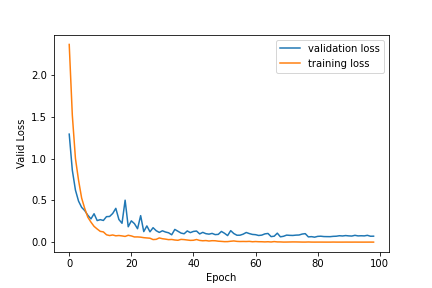
\includegraphics[width = \gws cm]{epoch_valid_loss_resnet101_2.png}
\caption{Validation loss and training loss for Resnet101 over 100 epochs}\label{fig:epoch_valid_loss_resnet101_2}
     \end{subfigure}
\begin{subfigure}{0.5\textwidth}
     \centering
	    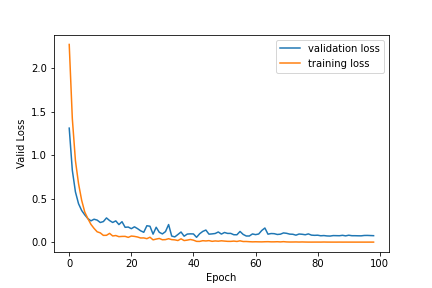
\includegraphics[width = \gws cm]{epoch_valid_loss_resnet152_2.png}
\caption{Validation loss and training loss for Resnet152 over 100 epochs}\label{fig:epoch_valid_loss_resnet152_2}
     \end{subfigure}  
     \caption{Training loss and validation loss of Resnet101 and Resnet152 over 100 epochs on the  'plant\_seedlings\_v2' dataset and the gray-scale pictures}
        \label{fig:tran_valid_loss_seeds_res_100_2}
\end{figure}

\chapter{Conclusion}
\section{Future Work}
This paper leaves many interrogatives open which need to be explored in future works. \\
First of all, in chapter \ref{char_nn}, we only investigated some of the characteristics which neural networks possess and can be correlated with each other. For example, we did not focus on parameters which influence the performances of the networks, like for i.g.learning rate, batch size or throughput. It is left for further studies to identify other characteristics that can be worth studying to find more correlations.\\
In chapter \ref{ana_models}, only techniques related to measuring execution time have been described. However, benchmarks are also used to measure other metrics, such us energy consumption or memory use. It is left for future work to find better techniques to precisely measure and monitor them, as they are also of the highest importance especially for devices with low on-board resources. Furthermore, in this paper we mainly focused on Linux, therefore purposely neglecting other operating systems and micro-controllers and only mentioning some techniques to run benchmarks on mobile devices running Android. 
The study of measurements techniques for other systems is also left for future work. \\
In chapter \ref{ana_char}, we run the benchmarking tool only on two examples. Even though we obtained promising results, we left some interrogatives behind. Firstly, we only run the tool with model from three different CNN architectures. Secondly, we did not investigate how ad-hoc-created models will behave under the conditions we defined. Thirdly, the experiments we made have been run without any augmentation or optimization on both the models and datasets. The models have been trained with the standard batch size, learning rate and were not pre-trained.In addition, they have been trained with full precision. It is left for further investigations to prove if further correlations can be found using different models and different optimizations.\\
Finally, we only investigated if, and which, correlations can be found studying the performance and the behaviour of neural networks. However, this serves only as a starting point for further applications and we did not investigate if these correlations can be used to optimize real world applications. Further research would be needed to prove it. 

\section{Conclusion}

%Literaturverzeichnis
\newpage
\lhead{}
\rhead{\leftmark}


\renewcommand*\bibname{References}
\addcontentsline{toc}{chapter}{References}
\bibliography{bib}
\bibliographystyle{alpha}

\appendix

\chapter{Appendix}
\begin{figure}[ht]
       \centering 
	    \includegraphics[width = 10 cm]{resnet_arch_full.png}
        \caption[Example of the architecture of residual networks]{ Left: the VGG-19 model [41] (19.6 billion FLOPs) as a reference. Middle: a plain network with 34 parameter layers (3.6 billion FLOPs). Right: a residual network with 34 parameter layers (3.6 billion FLOPs). The dotted shortcuts increase dimensions.\cite{DBLP:journals/corr/HeZRS15}}
         \label{fig:resnet_arch_full}
\end{figure}
\begin{figure}[ht]
       \centering 
	    \includegraphics[width = 13 cm]{fastest_files.png}
        \caption{Histogram of the fastest files}
         \label{fig:fastest_files_his}
\end{figure}

\begin{figure}[ht]
       \centering 
	    \includegraphics[width = 13 cm]{slowest_files.png}
        \caption{Histogram of the slowest files}
         \label{fig:slowest_files_his}
\end{figure}





\end{document}
